\documentclass[a4paper,11pt]{book}
% Préambule LaTeX - Configuration du document
% Conforme au template officiel UNamur Master Sciences Informatiques

% ============================================================================
% PACKAGES DE BASE
% ============================================================================

% Encodage et langue
\usepackage[utf8]{inputenc}
\usepackage[T1]{fontenc}
\usepackage[sfdefault]{atkinson}  % Police Atkinson Hyperlegible (obligatoire UNamur)
\usepackage[french]{babel}

% Marges et mise en page (conformes template UNamur)
\usepackage[top=2cm, bottom=2.5cm, left=2cm, right=2cm]{geometry}
\usepackage{setspace}
\onehalfspacing  % Interligne 1.5

% Polices et typographie
\renewcommand{\familydefault}{\sfdefault}
\usepackage{microtype}  % Amélioration typographie

% ============================================================================
% PACKAGES GRAPHIQUES
% ============================================================================

\usepackage{graphicx}
\usepackage{float}
\usepackage[dvipsnames]{xcolor}
\usepackage{tikz}  % Pour page de couverture
\usepackage{fancybox}

% Chemin vers les figures
\graphicspath{{figures/}{img/}}

% ============================================================================
% PACKAGES MATHÉMATIQUES
% ============================================================================

\usepackage{amsmath}
\usepackage{amssymb}
\usepackage{amsthm}

% ============================================================================
% PACKAGES TABLEAUX
% ============================================================================

\usepackage{array}
\usepackage{booktabs}
\usepackage{longtable}
\usepackage{multirow}

% ============================================================================
% PACKAGES LISTES ET ÉNUMÉRATIONS
% ============================================================================

\usepackage{enumitem}
\usepackage{pifont}

% ============================================================================
% PACKAGES BIBLIOGRAPHIE
% ============================================================================

\usepackage[backend=biber,style=numeric,sorting=none,maxbibnames=99]{biblatex}
\addbibresource{bibliography.bib}

% ============================================================================
% PACKAGES LIENS ET RÉFÉRENCES
% ============================================================================

\usepackage[hidelinks]{hyperref}
\usepackage{url}
\usepackage{cleveref}

\hypersetup{
    colorlinks=false,
    linkcolor=black,
    citecolor=black,
    urlcolor=blue,
    pdftitle={Mesures DNS dans l'espace et le temps},
    pdfauthor={Olivier Gautier},
    pdfsubject={Master 60 Sciences Informatiques - UNamur},
    pdfkeywords={DNS, RIPE Atlas, mesures distribuées, géolocalisation}
}

% Configuration des URLs
\urlstyle{same}

% ============================================================================
% PACKAGES CODE SOURCE
% ============================================================================

\usepackage{listings}
\usepackage[linesnumbered,ruled,vlined]{algorithm2e}

% Configuration listings - Couleurs
\definecolor{codebg}{rgb}{0.97,0.97,0.97}
\definecolor{javakeyword}{RGB}{0,0,180}
\definecolor{javacomment}{RGB}{0,128,0}
\definecolor{javastring}{RGB}{163,21,21}

% Style Python
\lstdefinestyle{python}{
  language=Python,
  backgroundcolor=\color{codebg},
  basicstyle=\ttfamily\small,
  keywordstyle=\color{blue}\bfseries,
  commentstyle=\color{gray}\itshape,
  stringstyle=\color{orange},
  showstringspaces=false,
  numbers=left,
  numberstyle=\tiny\color{gray},
  numbersep=10pt,
  frame=single,
  tabsize=4,
  captionpos=b,
  breaklines=true,
  breakatwhitespace=true
}

% Style Bash
\lstdefinestyle{bash}{
  language=bash,
  backgroundcolor=\color{codebg},
  basicstyle=\ttfamily\small,
  keywordstyle=\color{blue}\bfseries,
  commentstyle=\color{gray}\itshape,
  stringstyle=\color{orange},
  showstringspaces=false,
  numbers=left,
  numberstyle=\tiny\color{gray},
  numbersep=10pt,
  frame=single,
  breaklines=true
}

% Style JSON
\lstdefinelanguage{json}{
  morestring=[b]",
  morestring=[d]',
  literate=
   *{0}{{{\color{blue}0}}}{1}
    {1}{{{\color{blue}1}}}{1}
    {2}{{{\color{blue}2}}}{1}
    {3}{{{\color{blue}3}}}{1}
    {4}{{{\color{blue}4}}}{1}
    {5}{{{\color{blue}5}}}{1}
    {6}{{{\color{blue}6}}}{1}
    {7}{{{\color{blue}7}}}{1}
    {8}{{{\color{blue}8}}}{1}
    {9}{{{\color{blue}9}}}{1}
    {:}{{{\color{red}:}}}{1}
    {,}{{{\color{red},}}}{1}
    {\{}{{{\color{red}\{}}}{1}
    {\}}{{{\color{red}\}}}}{1}
    {[}{{{\color{red}[}}}{1}
    {]}{{{\color{red}]}}}{1}
    {true}{{{\color{purple}true}}}{4}
    {false}{{{\color{purple}false}}}{5}
    {null}{{{\color{purple}null}}}{4},
}

\lstdefinestyle{json}{
  language=json,
  backgroundcolor=\color{codebg},
  basicstyle=\ttfamily\small,
  keywordstyle=\color{blue},
  stringstyle=\color{orange},
  showstringspaces=false,
  numbers=left,
  numberstyle=\tiny\color{gray},
  numbersep=10pt,
  frame=single,
  breaklines=true,
  captionpos=b
}

% ============================================================================
% EN-TÊTES ET PIEDS DE PAGE
% ============================================================================

\usepackage{fancyhdr}

\pagestyle{fancy}
\fancyhf{}
\fancyhead[L]{\nouppercase{\leftmark}}
\fancyhead[R]{\thepage}
\renewcommand{\headrulewidth}{1pt}
\renewcommand{\footrulewidth}{0pt}

% Style pour pages de chapitre
\fancypagestyle{plain}{
    \fancyhf{}
    \fancyfoot[C]{\thepage}
    \renewcommand{\headrulewidth}{0pt}
}

% Hauteur en-tête
\setlength{\headheight}{13.59999pt}

% ============================================================================
% PACKAGES CAPTIONS
% ============================================================================

\usepackage{caption}
\usepackage{subcaption}

\captionsetup{
    font=small,
    labelfont=bf,
    textfont=it
}

% ============================================================================
% CONFIGURATION DOCUMENT
% ============================================================================

% Profondeur table des matières
\setcounter{tocdepth}{2}
\setcounter{secnumdepth}{3}

% Espacement paragraphes
\setlength{\parskip}{0.5em}
\setlength{\parindent}{0pt}

% Justification
\usepackage{ragged2e}

% ============================================================================
% COMMANDES PERSONNALISÉES
% ============================================================================

% Commande pour le symbole de référence
\newcommand{\refmark}[1]{\textsuperscript{\cite{#1}}}

% Commande pour faciliter les références
\newcommand{\figref}[1]{Figure~\ref{#1}}
\newcommand{\tabref}[1]{Tableau~\ref{#1}}
\newcommand{\chapref}[1]{Chapitre~\ref{#1}}
\newcommand{\secref}[1]{Section~\ref{#1}}

% ============================================================================
% FIN DU PRÉAMBULE
% ============================================================================


%%%%%%%%%%%%%%%%%%%%%%%%%%%%%%%%%%%%%%%%%%%%%%%%%%%%%%%%%%%%%%%%%%%%%%%%%%%%%%%%%%%%%%%%
%% TITRE DU MEMOIRE
%%%%%%%%%%%%%%%%%%%%%%%%%%%%%%%%%%%%%%%%%%%%%%%%%%%%%%%%%%%%%%%%%%%%%%%%%%%%%%%%%%%%%%%%

\newcommand{\titreMemoire}{Mesures DNS dans l'espace et le temps}

%%%%%%%%%%%%%%%%%%%%%%%%%%%%%%%%%%%%%%%%%%%%%%%%%%%%%%%%%%%%%%%%%%%%%%%%%%%%%%%%%%%%%%%%
%% AUTEUR(S) DU MEMOIRE
%%%%%%%%%%%%%%%%%%%%%%%%%%%%%%%%%%%%%%%%%%%%%%%%%%%%%%%%%%%%%%%%%%%%%%%%%%%%%%%%%%%%%%%%

\newcommand{\auteurMemoire}{Olivier Gautier}

%%%%%%%%%%%%%%%%%%%%%%%%%%%%%%%%%%%%%%%%%%%%%%%%%%%%%%%%%%%%%%%%%%%%%%%%%%%%%%%%%%%%%%%%
%% DIPLOME
%%%%%%%%%%%%%%%%%%%%%%%%%%%%%%%%%%%%%%%%%%%%%%%%%%%%%%%%%%%%%%%%%%%%%%%%%%%%%%%%%%%%%%%%
%% Master 60
\newcommand{\diplome}{Mémoire présenté en vue de l'obtention du grade de Master 60 en Sciences Informatiques}

%%%%%%%%%%%%%%%%%%%%%%%%%%%%%%%%%%%%%%%%%%%%%%%%%%%%%%%%%%%%%%%%%%%%%%%%%%%%%%%%%%%%%%%%
%% ANNEE ACADEMIQUE
%%%%%%%%%%%%%%%%%%%%%%%%%%%%%%%%%%%%%%%%%%%%%%%%%%%%%%%%%%%%%%%%%%%%%%%%%%%%%%%%%%%%%%%%

\newcommand{\anneeacademique}{2025-2026}

%%%%%%%%%%%%%%%%%%%%%%%%%%%%%%%%%%%%%%%%%%%%%%%%%%%%%%%%%%%%%%%%%%%%%%%%%%%%%%%%%%%%%%%%
%% PROMOTEUR & (CO-PROMOTEUR)
%%%%%%%%%%%%%%%%%%%%%%%%%%%%%%%%%%%%%%%%%%%%%%%%%%%%%%%%%%%%%%%%%%%%%%%%%%%%%%%%%%%%%%%%

\newcommand{\promoteur}{F. Rochet}
\newcommand{\copromoteur}{P. Luycx -- J. Dejaeghere}

%%%%%%%%%%%%%%%%%%%%%%%%%%%%%%%%%%%%%%%%%%%%%%%%%%%%%%%%%%%%%%%%%%%%%%%%%%%%%%%%%%%%%%%%

\begin{document}
\renewcommand{\footrulewidth}{0pt}
\fancyhf{}
%%%%%%%%%%%%%%%%%%%%%%%%%%%%%%%%%%%%%%%%%%%%%%%%%%%%%%%%%%%%%%%%%%%%%%%%%%
%% NE PAS EDITER CE FICHIER
%%%%%%%%%%%%%%%%%%%%%%%%%%%%%%%%%%%%%%%%%%%%%%%%%%%%%%%%%%%%%%%%%%%%%%%%%%



\fancyfoot[C]{} % Retrait footer
    \pagestyle{fancyplain}
    \begin{tikzpicture}[remember picture,overlay]
        \node[anchor=north west,yshift=-30pt,xshift=30pt]
            at (current page.north west)
            {
\includegraphics[height=5cm]{img/FAC_informatique.png}};
    \end{tikzpicture}
    
\centerline{UNIVERSITÉ DE NAMUR}
\centerline{Faculté d'informatique}
\centerline{Année académique \anneeacademique}

\vspace{4cm}

\begin{center}
	\fbox{ \begin{minipage}[c][5.4cm]{9.6cm}
            \large
            \begin{spacing}{1.2}
                \begin{center}
                    \centering \textbf{\titreMemoire}
                    \vspace{1cm}
                    
                    \auteurMemoire
                \end{center}
            \end{spacing}
        \end{minipage}}
\end{center}

    % ==> CADRE A COMPLETER
    \vspace{2.8cm}
    \centerline{
        \begin{minipage}[c][3cm]{9.6cm} 
            \begin{spacing}{2}
                \begin{center}
                    \leftline{........................ (Signature pour approbation du dépôt - REE art. 40)}
                    \leftline{Promoteur : \promoteur}
                    \leftline{Co-promoteurs : \copromoteur}
                \end{center}
            \end{spacing}
        \end{minipage}
    }

    \vspace{2cm}
    \centering\mbox{
        \begin{minipage}[c][5cm]{9.6cm}
            \begin{spacing}{2}
                \begin{center}
                    \vspace{6.4cm}
                    \centerline{\large\diplome}
                    %\newline
                    \vspace{1.6cm}
                    \centerline{ Faculté d'Informatique --- Université de Namur}
                   % \newline 
                    \centerline{ RUE GRANDGAGNAGE, 21 $\bullet$ B-5000 NAMUR  $\bullet$ BELGIUM}
                \end{center}
            \end{spacing}
        \end{minipage}
    }


%%%%%%%%%%%%%%%%%%%%%%%%%%%%%%%%%%%%%%%%%%%%%%%%%%%%%%%%%%%%%%%%%%%%%%%%%%%%%%%%%%%%%%%%%

\justifying
\pagestyle{empty} 
\onehalfspacing 

\clearpage\newpage\hbox{ }\clearpage\newpage

\noindent\textbf{\huge Remerciements}
\bigskip

\begin{quote}
\hl{\textit{To be completed}}
\end{quote}

\clearpage\newpage\hbox{ }\clearpage\newpage

\noindent\textbf{\huge Résumé}
\bigskip

\begin{quote}
\hl{\textit{To be completed}}
\end{quote} 
\bigskip
\noindent\textbf{Mots-clés} : DNS, mesures distribuées, géolocalisation, CDN, RIPE Atlas, diversité géographique, Tranco

\vspace{0.75cm}

\noindent\textbf{\huge Abstract}
\bigskip

\begin{quote}
\hl{\textit{To be completed}}
\end{quote}
\bigskip
\noindent\textbf{Keywords} : DNS, distributed measurements, geolocation, CDN, RIPE Atlas, geographic diversity, Tranco

\clearpage\newpage\hbox{ }\clearpage\newpage

\tableofcontents

\clearpage\newpage\hbox{ }\clearpage\newpage
\pagestyle{empty}

\section*{Acronymes}

\begin{acronym}[DNSSEC]
        \acro{A}{IPv4 Address Record}
        \acro{AAAA}{IPv6 Address Record}
        \acro{ARIN}{American Registry for Internet Numbers}
        \acro{AS}{Autonomous System}
        \acro{BGP}{Border Gateway Protocol}
        \acro{CDN}{Content Delivery Network}
        \acro{CNAME}{Canonical Name Record}
        \acro{DDoS}{Distributed Denial of Service}
        \acro{DOI}{Digital Object Identifier}
        \acro{DKIM}{DomainKeys Identified Mail}
        \acro{DMARC}{Domain-based Message Authentication, Reporting, and Conformance}
        \acro{DNS}{Domain Name System}
        \acro{DNSSEC}{DNS Security Extensions}
        \acro{ECS}{Extension Mechanisms for DNS Client Subnet}
        \acro{FAIR}{Findability, Accessibility, Interoperability, and Reuse}
        \acro{HTTP}{HyperText Transfer Protocol}
        \acro{IP}{Internet Protocol}
        \acro{IPv4}{Internet Protocol version 4}
        \acro{IPv6}{Internet Protocol version 6}
        \acro{ISP}{Internet Service Provider}
        \acro{IXPs}{Internet Exchange Points}
        \acro{MX}{Mail Exchanger Record}
        \acro{NS}{Name Server Record}
        \acro{NSID}{Name Server Identifier}
        \acro{PoP}{Point of Presence}
        \acro{PoPs}{Points of Presence}
        \acro{RD}{Recursion Desired}
        \acro{RIPE NCC}{Réseaux IP Européens – Network Coordination Centre}
        \acro{RR}{Resource Record}
        \acro{RTT}{Round-Trip Time}
        \acro{SPF}{Sender Policy Framework}
        \acro{TLD}{Top-Level Domain}
        \acro{TTL}{Time To Live}
        \acro{TXT}{Text Record}
        \acro{UDP}{User Datagram Protocol}
 \end{acronym}

\clearpage\newpage\hbox{ }\clearpage\newpage

\fancyhf{}
\fancyfoot[L]{\nouppercase{\leftmark}}
\fancyfoot[R]{\thepage}
\renewcommand{\headrulewidth}{0pt}
\renewcommand{\footrulewidth}{0.4pt}
\pagestyle{fancy}

\chapter{Introduction}
\label{ch:introduction}

\section{Context and Motivation}
\label{sec:1.1}

The \ac{DNS}, specified by Mockapetris~\cite{RFC1034,RFC1035}, is the distributed directory service that translates domain names into \ac{IP} addresses and supports virtually every networked application on the Internet. Despite this criticality — illustrated by the Facebook \ac{DNS} outage of October 2021, which made the domain globally unresolvable for nearly six hours~\cite{Xu2023} — the \ac{DNS} has historically received less systematic measurement attention than other infrastructure layers. The most comprehensive longitudinal \ac{DNS} measurement system, OpenINTEL~\cite{vanRijswijk2016}, measures over 50\% of the global \ac{DNS} namespace daily but does so from a single vantage point in the Netherlands, leaving the geographic dimension of \ac{DNS} responses entirely uncharacterised.

\ac{DNS} data is also fundamentally ephemeral: every \ac{RR} carries a \ac{TTL} after which it is discarded~\cite{RFC1034,RFC1035}. Zone administrators can change records at any time, and the \ac{DNS} infrastructure retains no trace of previous configurations. This ephemerality motivates longitudinal archival: security researchers need historical \ac{DNS} data to reconstruct the evolution of malicious infrastructure~\cite{vanderToorn2018}; network measurement researchers need longitudinal,
geographically distributed data to characterise anycast routing and \ac{CDN} behaviour~\cite{Bortzmeyer2013,Hours2016}; infrastructure analysts need longitudinal datasets to track provider migrations and \ac{DNSSEC} deployment trends~\cite{vanRijswijk2016}.

Beyond the temporal dimension, \ac{DNS} responses exhibit a geographic dimension that single-vantage point measurement cannot observe. Three mechanisms produce this variation: (1) \textbf{\ac{CDN}-based routing} — authoritative servers return different \ac{IP} addresses depending on the inferred location of the querying resolver, directing clients to the nearest edge cluster~\cite{Li2025,Hours2016}; (2) \textbf{\ac{IP} anycast} — the same global \ac{IP} address is announced from multiple geographically distributed \ac{PoPs}, so queries from different regions reach different physical instances~\cite{Bortzmeyer2013,Koch2021}; and (3) \textbf{\ac{ECS}}~\cite{RFC7871} — the resolver embeds a truncated client \ac{IP} prefix in the query, enabling the \ac{CDN} to route by end-client location rather than resolver location~\cite{Wang2018}. 

The proportion of popular domains that return geographically differentiated responses, the magnitude and temporal stability of that differentiation, and the mechanisms that drive it remain empirically uncharacterised at population scale. This is the research gap this thesis addresses.

\bigskip
\section{DNS Resolution: a Brief Overview}
\label{sec:1.2}

Every time a browser contacts a website, a short chain of queries unfolds before any data is exchanged. \ac{DNS} handles the translation from human-readable names to numeric \ac{IP} addresses, through a hierarchy of servers distributed across the globe.

The namespace is divided into zones — administrative units, each delegated to one or more authoritative name servers that hold the canonical records for that portion of the tree. These records (\ac{RR}s) come in typed forms: an \ac{A} record binds a name to an \ac{IPv4} address; each record also carries a \ac{TTL}, after which any cached copy is considered expired.

In practice, a client application never contacts an authoritative server directly. The query goes first to the operating system's stub resolver, which forwards it to a recursive resolver — the \ac{ISP}'s, or a public alternative such as Google (8.8.8.8) or Cloudflare (1.1.1.1). If the recursive resolver holds a valid cached answer, it returns it immediately. If not, it iterates down the hierarchy — from the root servers through the appropriate \ac{TLD} server, down to the domain's own authoritative servers — retrieves the answer, caches it for the \ac{TTL} duration, and passes it back to the client. Figure~\ref{fig:DNS_resolution} illustrates this process.

\begin{figure}[tp]
  \centering
  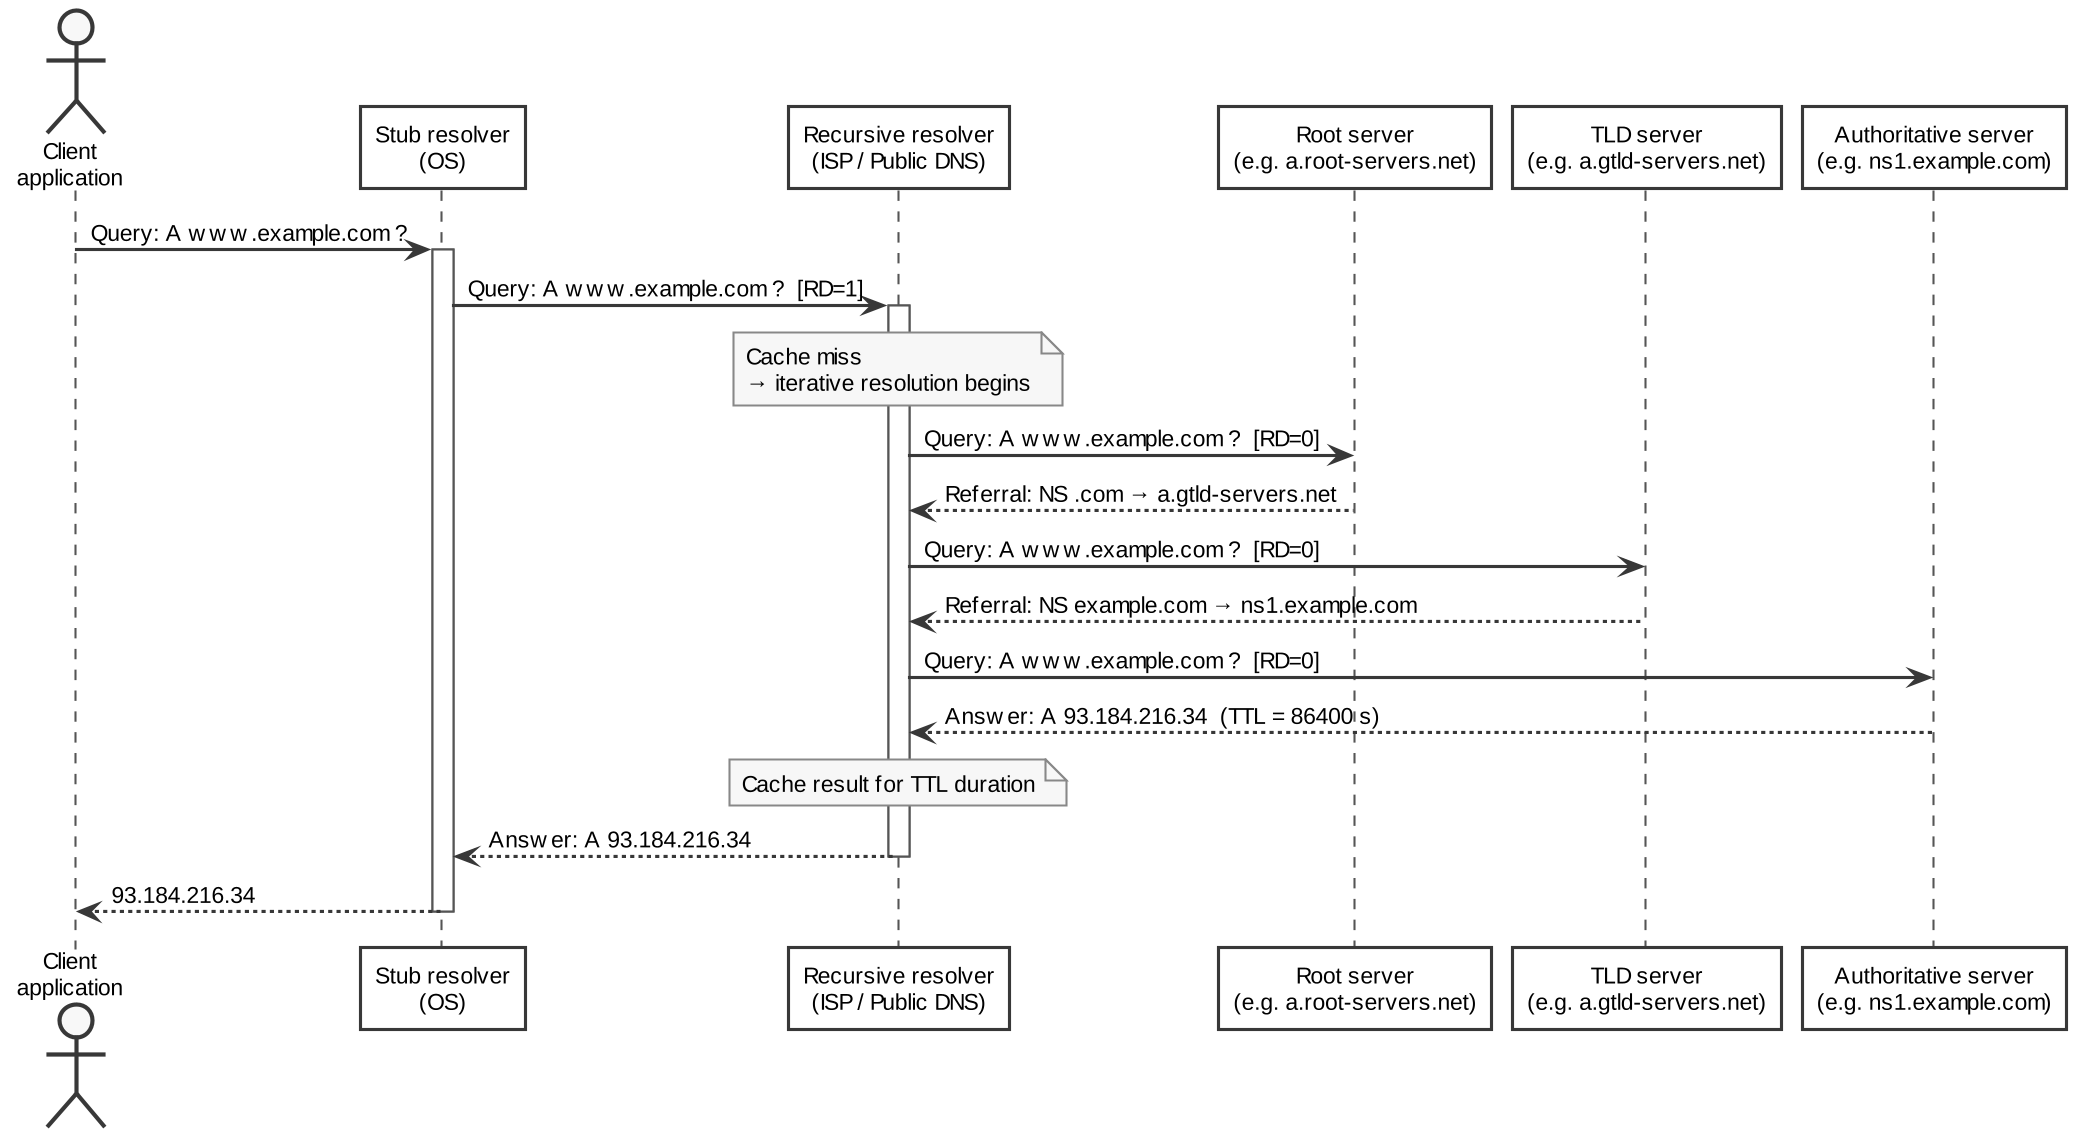
\includegraphics[width=0.92\linewidth]{figures/fig1_dns_resolution.png}
  \caption{Iterative \ac{DNS} resolution process. The client-side resolver (stub) forwards the query to a recursive resolver, which performs three successive referral queries (root $\rightarrow$ \ac{TLD} $\rightarrow$ authoritative) before returning the final answer. The \ac{TTL} field in the authoritative response governs how long the recursive resolver caches the result.}
  \label{fig:DNS_resolution}
\end{figure}

This architecture has two consequences central to this thesis. First, the recursive resolver acts as a geographic proxy: from the authoritative server's perspective, all queries originating from the same recursive resolver appear to come from a single location, regardless of where the end-users actually are. \ac{CDN} operators exploit this to tailor answers by resolver location. Second, because any resolver can query any authoritative server, it is possible to measure how authoritative servers respond to queries from different geographic vantage points — which is precisely the approach taken in Chapter~\ref{ch:method}.

\bigskip
\section{Research Questions and Objectives}
\label{sec:1.3}

This thesis addresses the following main research question:

\textit{How can one design and deploy a distributed \ac{DNS} measurement system that captures the geographic and temporal diversity of \ac{DNS} responses for the most popular domains on the web, in a manner that is ethically sound, reproducible, and useful to the research community?}

Four operational sub-questions guide the empirical analysis:

\textbf{Q1 — Geographic diversity}: What proportion of popular domains return different \ac{DNS} responses depending on query origin, and which mechanisms (\ac{CDN} routing, anycast, \ac{ECS}) explain the differentiation? 

Measuring the full Tranco Top-10K would require on the order of 10,000 concurrent RIPE Atlas measurements, far exceeding typical account limits; this thesis therefore focuses on the Tranco Top-250, which concentrates on the highest-traffic domains where geographic differentiation is most prevalent and the findings most practically relevant.


\textbf{Q2 — Temporal stability}: What is the temporal stability of \ac{DNS} responses at day, week, and month timescales over the measurement period?

\textbf{Q3 — RIPE Atlas geographic bias}: Do the documented geographic biases of the RIPE Atlas probe distribution~\cite{Bajpai2017} (91\% of probes in Europe/North America) significantly affect the ability to observe \ac{DNS} geographic variation?

\textbf{Q4 — Resolver impact}: Do the three major public \ac{DNS} resolvers (Google 8.8.8.8, Cloudflare 1.1.1.1, Quad9 9.9.9.9) return consistent \ac{DNS} responses for the same domain queried from the same geographic location, and how large is the inter-resolver divergence?

To answer these questions, the thesis designs, implements, and operates a measurement system that: (1) measures the Tranco Top 250 domains~\cite{LePochat2019} daily over 50 days — a duration chosen to cover at least one complete monthly cycle, enabling analysis of \ac{DNS} stability at the day, week, and month timescales required by Q2; (2) collects measurements from $\approx$200 globally distributed RIPE Atlas probes selected via RIPE Atlas geographic zone-based distribution; (3) archives results in Parquet format following \ac{FAIR} data principles; and (4) analyses the dataset to produce quantitative answers to Q1–Q4. The measurement design complies with the RIPE Atlas ethical guidelines~\cite{Kisteleki2016}: all queried domains are publicly accessible, measurement frequency respects \ac{DNS} \ac{TTL}s, and no politically sensitive content is included.

\bigskip
\section{Thesis Structure}
\label{sec:1.4}

\textbf{Chapter~\ref{ch:state-of-the-art}} reviews the state of the art across five domains: \ac{DNS} measurement paradigms and the OpenINTEL infrastructure; the RIPE Atlas platform and its biases; anycast routing and \ac{NSID}-based instance identification; \ac{CDN} \ac{DNS} routing and \ac{ECS}; and domain ranking lists, concluding with a gap analysis.

\textbf{Chapter~\ref{ch:method}} describes the full measurement methodology: Tranco corpus configuration, RIPE Atlas probe selection and stratification, \ac{DNS} measurement parameters, data collection pipeline, and Parquet storage architecture.

\textbf{Chapter~\ref{ch:results}} presents the empirical results of the measurement campaign: dataset statistics and answers
to Q1–Q4 with quantitative evidence and visualisations.

\textbf{Chapter~\ref{ch:conclusion}} discusses the results in light of the literature, evaluates study limitations, and draws
conclusions with future research directions.
\chapter{State of the Art}
\label{ch:state-of-the-art}

\section{The DNS System: Background}
\label{subsec:2.1}

The \ac{DNS} is the distributed directory that translates human-readable names into machine-readable information — primarily \ac{IP} addresses~\cite{RFC1034,RFC1035}. Its hierarchy mirrors the delegation of administrative authority: the root zone delegates to \ac{TLD}s, which delegate to authoritative name servers for individual domains. Resolution is performed by a recursive resolver acting on behalf of clients — contacting root, \ac{TLD}, and authoritative servers in sequence and caching results for the duration of each record’s \ac{TTL}.

Every \ac{RR} includes a \ac{TTL} that defines how long it remains in the cache. While \ac{CDN}s rely on short \ac{TTL}s (often 60 seconds or less) to dynamically reroute traffic, stable infrastructures typically set \ac{TTL}s of 24 hours or longer. This variance introduces critical challenges for active measurements. Relying on a recursive resolver risks retrieving outdated cached data. And different cache states across probes can easily be misinterpreted as geographic routing variations. Querying authoritative servers directly eliminates both of these confounding factors.

\subsection{Resource Record Types Relevant to Measurement Studies}
\label{sec:2.1.1}

\ac{DNS} stores information in typed Resource Records, each serving a distinct purpose \cite{RFC1035}. The record types most relevant to distributed measurement studies are:

\textbf{\ac{A} and \ac{AAAA} records} map a domain name to an \ac{IPv4} or \ac{IPv6} address respectively. A single name may have multiple \ac{A} or \ac{AAAA} records, enabling load distribution through round-robin responses and geographic routing through location-aware \ac{DNS} (different addresses returned depending on the querying resolver's location). This geographic differentiation in \ac{A}/\ac{AAAA} responses is one of the primary phenomena this thesis investigates.

\textbf{\ac{NS} records} designate the authoritative name servers responsible for a \ac{DNS} zone and are essential for identifying the \ac{DNS} infrastructure provider responsible for a domain. Van Rijswijk-Deij~\cite{vanRijswijk2016} include \ac{NS} records in the OpenINTEL standard query set because changes in \ac{NS} delegation reveal infrastructure migrations and provider switches.

\textbf{\ac{MX} records} designate the mail-handling servers for a domain. Van Rijswijk-Deij~\cite{vanRijswijk2016} use longitudinal \ac{MX} analysis as one of two case studies for OpenINTEL, tracking the adoption of cloud email services (Google Workspace, Microsoft Exchange Online, Yahoo Mail) across tens of millions of domains over a ten-month period.

\textbf{\ac{CNAME} records} create an alias pointing from one name to another canonical name. \ac{CDN}s make extensive use of \ac{CNAME} chains: a customer domain (\texttt{www.shop.example}) points to a \ac{CDN}-managed name (\texttt{shop.cdn-provider.net}), allowing the \ac{CDN} to update routing without requiring the customer to change their \ac{DNS} configuration. The same mechanism is used by \ac{DDoS} protection services to divert traffic through their scrubbing infrastructure~\cite{Jonker2016}.

\textbf{DNSKEY, DS, and RRSIG records} serve as the core cryptographic pillars of \ac{DNSSEC}, anchoring public keys, delegation signers, and digital signatures. To track \ac{DNSSEC} deployment and key management strategies on a global scale, Van Rijswijk-Deij~\cite{vanRijswijk2016} integrated this entire triad into the OpenINTEL query framework. By analyzing this specific longitudinal dataset, the authors were able to expose systemic key rollover failures that remained completely hidden during standard, point-in-time assessments.

\textbf{\ac{TXT} records} carry free-text information and are used for \ac{SPF}, \ac{DKIM}, \ac{DMARC} configuration, and domain validation tokens for certificate authorities. Table~\ref{tab:rr_types} summarises the record types relevant to this thesis's measurement campaign.

\begin{table}[H]
\centering
\small
\begin{tabularx}{\linewidth}{p{1.8cm} p{4.1cm} X}
\toprule
\textbf{Type} & \textbf{Content} & \textbf{Relevance for distributed \ac{DNS} measurement} \\
\midrule
\ac{A}     & \ac{IPv4} address(es)                  & Core observable: geographic variation in returned \ac{IP}s indicates \ac{CDN} routing or anycast \\
\ac{AAAA}  & \ac{IPv6} address(es)                  & Parallel to \ac{A}; anycast routing may differ between \ac{IPv4} and \ac{IPv6}~\cite{Bortzmeyer2013} \\
\ac{NS}    & Authoritative name server names   & Identifies \ac{DNS} provider; enables provider migration tracking and centralisation analysis~\cite{Xu2023} \\
\ac{CNAME} & Canonical name alias              & \ac{CDN} delegation chain; resolving the chain reveals the \ac{CDN} operator behind a domain \\
\ac{MX}    & Mail server hostname(s)           & Cloud email adoption tracking~\cite{vanRijswijk2016}; not geographically differentiated \\
\ac{TXT}   & Free-form text                    & \ac{SPF}/\ac{DKIM}/\ac{DMARC} policy; domain ownership verification \\
DNSKEY/DS & \ac{DNSSEC} public key / delegation & \ac{DNSSEC} deployment monitoring; broken chains cause SERVFAIL; 31\% of \ac{DNSSEC} domains have incomplete records~\cite{vanRijswijk2016,Chung2017} \\
\bottomrule
\end{tabularx}
\caption{\ac{DNS} \ac{RR} types relevant to distributed measurement studies. References: \cite{RFC1034,RFC1035}.}
\label{tab:rr_types}
\end{table}

\section{DNS Measurement Paradigms}
\label{sec:2.2}

Measuring \ac{DNS} behaviour at scale can be approached in fundamentally different ways, each with its own trade-offs in terms of coverage, geographic control, and ethical constraints. This section surveys the two main paradigms — passive and active measurement — along with the ethical framework that governs their use, and presents OpenINTEL as the reference large-scale active measurement infrastructure against which this thesis positions itself.

\textbf{Passive \ac{DNS}} captures queries and responses at existing resolvers or \ac{IXPs} without injecting artificial traffic. It reflects real user behaviour and is well suited for security forensics (botnet tracking, phishing detection via commercial services such as Farsight DNSDB). Its fundamental limitation for this thesis is geographic blindness: a passive sensor observes only traffic at its location~\cite{vanRijswijk2016}. It also cannot measure a predefined domain corpus, privacy constraints (GDPR) restrict retention granularity, and the resulting datasets are typically held by commercial operators (Farsight DNSDB, \ac{ISP}s), making them inaccessible for open academic research.

\textbf{Active \ac{DNS} measurement} deliberately sends queries from controlled vantage points, enabling full domain corpus coverage, geographic control, and reproducibility. Van Rijswijk-Deij~\cite{vanRijswijk2016} demonstrate that even at 1.85 billion daily queries for .com alone, well-paced active measurement represents only 0.3–1.6\% of authoritative server traffic — a negligible impact. Van der Toorn~\cite{vanderToorn2018} leverage 180 days of such data to detect snowshoe spam — a technique whereby spammers distribute sending across many domains to evade reputation-based blacklists — with 93\%+ precision and a 100-day lead over blacklists, a result exclusive to the active paradigm. Similarly, Jonker~\cite{Jonker2016} use 1.5 years of daily active measurements to track the adoption of \ac{DDoS} protection services across more than 50\% of the global namespace, revealing a 1.24$\times$ growth in adoption driven by large hosting providers — a trend invisible to any passive or point-in-time approach.

\textbf{Ethical framework}: As described by Kisteleki~\cite{Kisteleki2016}, RIPE Atlas measurement ethics align closely with the main principles of the Menlo Report (2012)~\cite{Bailey2012}, insisting that researchers must take full responsibility for the traffic generated by their probe hosts. In strict compliance with these principles, this thesis relies exclusively on publicly accessible Tranco domains. Furthermore, the experimental design intentionally avoids querying politically sensitive content and sets measurement frequency to respect standard \ac{DNS} \ac{TTL}s.

\textbf{OpenINTEL}~\cite{vanRijswijk2016}, developed at the University of Twente, measures every domain in a \ac{TLD} zone daily from a single vantage point in the Netherlands. It covers over 50\% of the global \ac{DNS} namespace, stores results in Apache Avro/Parquet, and has run continuously since March 2015. Its longitudinal data has supported studies of \ac{DNSSEC} key management failures~\cite{Chung2017}, \ac{DDoS} protection adoption~\cite{Jonker2016}, and cloud email migration~\cite{vanRijswijk2018blog}. Coverage expanded from the initial .com/.net/.org \ac{TLD}s (50\% of the global namespace) to all generic \ac{TLD}s by 2018, and the platform received the Research Data Netherlands Prize in November 2018~\cite{vanRijswijk2018blog}. Its explicit limitation is the single-vantage point architecture: whether a domain returns different \ac{IP} addresses to probes in Japan, Brazil, or South Africa is invisible to OpenINTEL — the primary motivation for the distributed approach of this thesis.


\section{Distributed Measurement: RIPE Atlas}
\label{sec:2.3}

Operated by a global network of volunteer-hosted hardware and software probes, RIPE Atlas offers the extensive spatial diversity that infrastructures like OpenINTEL lack. Data from 2024 shows the platform maintaining roughly 12,900 active probes (from a pool of over 30,000 registered devices) spanning 178 countries, which collectively yield around 1.3 billion daily measurement points~\cite{Nosyk2025}. Crucially, \ac{DNS} functionality is embedded as a native measurement type. Each probe perpetually tracks all 13 root server IP addresses, while custom user campaigns can be configured to target specific domains, resolvers, or record types. A detailed comparison between RIPE Atlas and alternative platforms is structured in Table~\ref{tab:platforms}.

\begin{table}[H]
\centering
\small
\begin{tabularx}{\linewidth}{p{2.6cm} r p{2.0cm} p{1.8cm} X}
\toprule
\textbf{Platform} & \textbf{Probes} & \textbf{Countries} & \textbf{\ac{DNS} native} & \textbf{Notes} \\
\midrule
RIPE Atlas       & $\approx$12,900 & 178 & Yes & Volunteer probes; credit economy; open academic access~\cite{Nosyk2025} \\
CAIDA Ark        & $\approx$170    & 60+ & No  & Topology-focused; data available on request to academic institutions; limited \ac{DNS} support~\cite{Bajpai2017} \\
SamKnows         & $\approx$70,000 & 50+ & No  & \ac{ISP}-deployed for regulators (FCC, Ofcom); not publicly accessible; broadband QoS focus~\cite{Bajpai2017} \\
PlanetLab        & $\approx$300    & 60+ & No  & Open to academic institutions (slice model); software VMs~\cite{Cicalese2015}; largely inactive since 2020 \\
BISmark          & $\approx$420    & 40+ & No  & Open source but limited access (Georgia Tech); home-network focus; limited geographic diversity~\cite{Bajpai2017} \\
\bottomrule
\end{tabularx}
\caption{Comparison of distributed Internet measurement platforms relevant to \ac{DNS} studies. Probe counts as of 2024 for RIPE Atlas~\cite{Nosyk2025} and approximately 2017 for others~\cite{Bajpai2017}. RIPE Atlas is the only platform with native \ac{DNS} measurement support and open academic access at global scale.}
\label{tab:platforms}
\end{table}

\textbf{Probe selection}: Bajpai~\cite{Bajpai2017} distinguish system tags (automatically derived from RIPE Atlas built-in measurements every four hours, reliable) from user tags (manually set by probe hosts; only 2.8\% ever update them, making them frequently stale). The recommended selection protocol is: filter by system tags (system-ipv4-works, system-resolves-a-correctly), then stratify geographically to compensate for the 91\% Europe/North America concentration. Holterbach~\cite{Holterbach2015} further document measurement interference: concurrent campaigns on the same probes introduce timing errors of 1–7 ms and temporal de-synchronisation of up to one hour. Scheduling at off-peak times and using repeated measurements mitigate both effects.

\textbf{Geographic bias}: A significant concentration of infrastructure exists in Germany and the USA, which combined host 28\% of all active probes. Conversely, regions such as Africa, Latin America, and Southeast Asia remain severely under-represented when compared to their actual Internet user populations~\cite{Nosyk2025}. This uneven global footprint is illustrated in Figure~\ref{fig:ripe_atlas_distribution}. Consequently, implementing strict geographic stratification during the probe selection phase becomes essential to accurately capture worldwide \ac{DNS} variations.

\begin{figure}[tp]
  \centering
  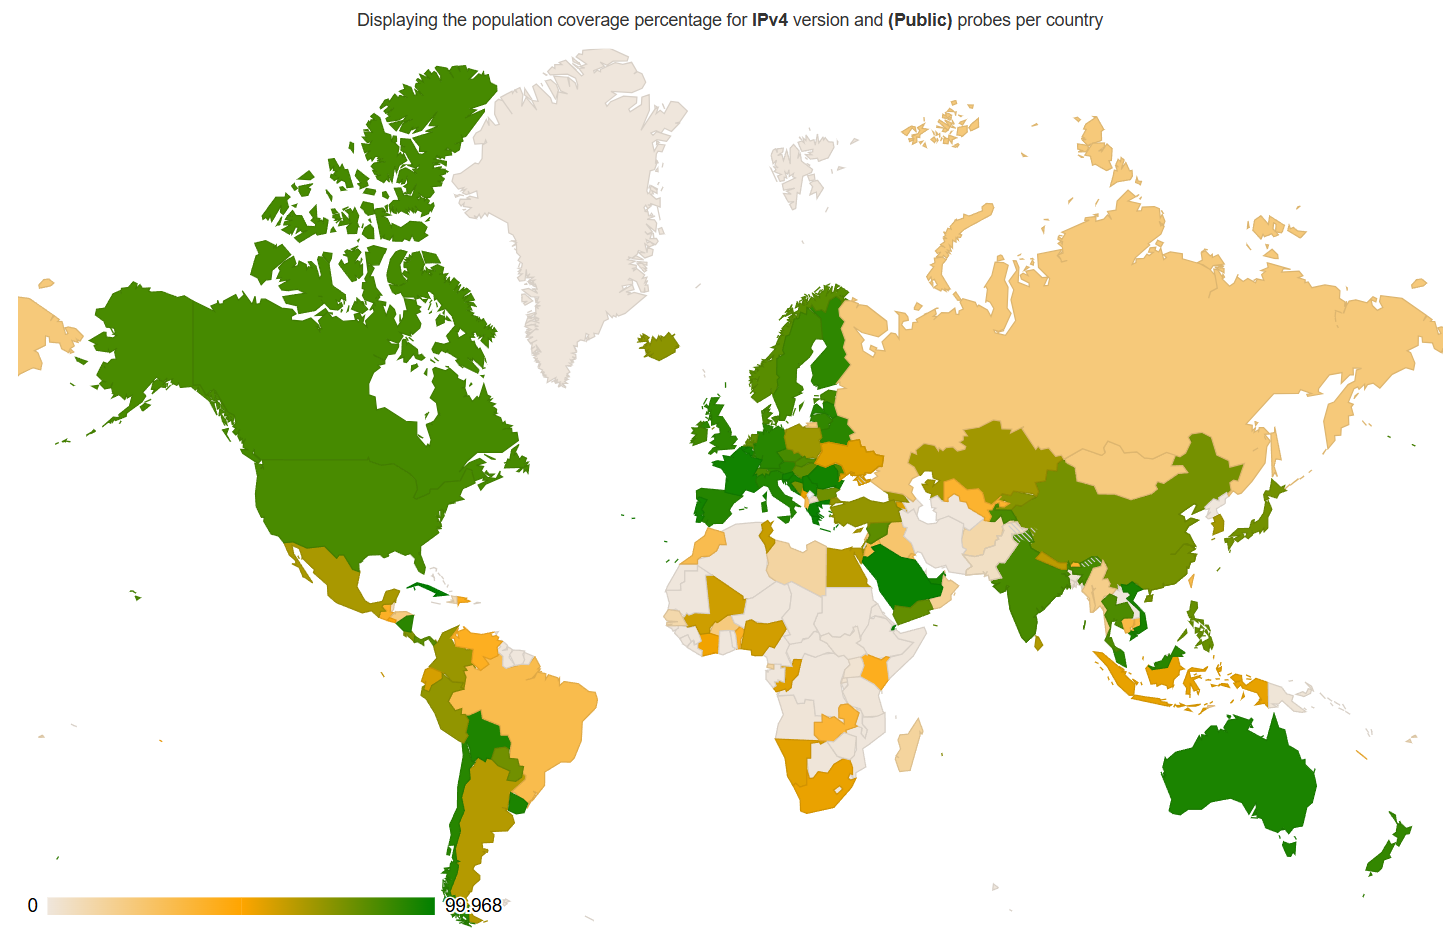
\includegraphics[width=0.90\linewidth]{figures/fig3b_ripe_atlas_distribution.png}
  \caption{Number of connected RIPE Atlas probes and anchors per country in March 30, 2026. Source: RIPE Atlas}
  \label{fig:ripe_atlas_distribution}
\end{figure}

\textbf{Measurement validity}: Jones~\cite{Jones2016} detect in-path transparent \ac{DNS} proxies in ten \ac{ISP}s: a Kenyan \ac{ISP}’s proxy answers root \ac{DNS} queries 23× faster than the actual B-root \ac{RTT} (14 ms vs. 318 ms). Nosyk~\cite{Nosyk2025} find that 69\% of Chinese probes fail to resolve Meta domains — geographic filtering, not measurement failure. These findings require two data quality steps: \ac{RTT} sanity checks to identify proxied probes, and cross-domain cross-temporal analysis to distinguish censorship from hardware failure. Boswell and Perkins~\cite{Boswell2024} further show that 3,092 internal domain names are actively used by RIPE Atlas probes, with 34.5\% at risk of name collision if their \ac{TLD} is globally delegated — a finding that underlines the need to validate probe resolution behaviour before including probes in \ac{DNS} corpus measurements.

\section{Anycast Routing in DNS}
\label{sec:2.4}

\ac{IP} anycast is the dominant routing architecture for \ac{DNS} root servers, \ac{TLD} servers, and major public resolvers (Google 8.8.8.8, Cloudflare 1.1.1.1). Probes at different geographic locations may contact physically different servers behind the same anycast \ac{IP}; the responses may differ in latency and, when servers are misconfigured or \ac{BGP} routing is suboptimal, in content. Three aspects of anycast are particularly relevant to distributed \ac{DNS} measurement: how to identify which physical instance answered a query, how \ac{BGP} topology shapes the geographic distribution of queries across instances, and how \ac{IPv4} and \ac{IPv6} routing can diverge for the same anycast address.

\textbf{Instance identification}: Mapping anycast topology requires identifying the specific physical server instance that handled a given query. Researchers typically deploy two complementary methods to achieve this. First, the \ac{NSID} option (~\cite{RFC5001}) instructs the responding server to include a unique identifier in its payload (such as \texttt{dns.th2.nic.fr} for the Paris instance of \texttt{d.nic.fr}). Alternatively, the id.server CHAOS query (~\cite{RFC4892}) prompts the server to return an airport-code-based identifier (e.g., ams, fra). Since CHAOS class records bypass standard caching mechanisms entirely, every query is guaranteed to reach the active, \ac{BGP}-routed instance~\cite{Finnegan2018}. Absent these tools, it is impossible to determine whether two probes receiving identical \ac{A} records are hitting the same or different routing destinations.

\textbf{\ac{BGP} attraction basins}: Once instance identity can be established, the question becomes: what governs which probes reach which instance? Bortzmeyer~\cite{Bortzmeyer2013} demonstrates for \texttt{d.nic.fr} that anycast routing is governed by \ac{BGP} peering topology rather than physical distance. For instance, while one might expect North American queries to be routed to the geographically closest available node, 55\% are sent to Paris and 33\% to Frankfurt — showing that network closeness in \ac{BGP} does not align with mileage. Finnegan~\cite{Finnegan2018} confirms this pattern for UncensoredDNS with 500 Atlas probes. This has a direct consequence for this thesis: geographic probe diversity does not guarantee instance diversity, and response differences between probes may reflect \ac{BGP} topology rather than intentional geographic routing.

\textbf{\ac{IPv4}/\ac{IPv6} divergence}: An additional layer of complexity stems from the fact that \ac{IPv4} and \ac{IPv6} \ac{BGP} routing tables operate independently. Consequently, queries targeting the exact same anycast prefix can end up routed to entirely different physical server instances depending on the \ac{IP} version utilized.
Bortzmeyer~\cite{Bortzmeyer2013} documents a reversal for \texttt{d.nic.fr}: Frankfurt is the dominant \ac{IPv6} instance (36\% of global queries) but subordinate in \ac{IPv4} (17\%). Dual-stack measurements must therefore be run and analysed separately to avoid conflating two distinct routing dimensions. Koch~\cite{Koch2021} further show that anycast inflation (routing to a suboptimal replica) affects over 95\% of users for at least one \ac{DNS} root letter, though its practical impact is negligible for root \ac{DNS} because root records are cached for six days.

\section{CDN Routing and EDNS Client Subnet}
\label{sec:2.5}

\ac{CDN}s use \ac{DNS} as the primary mechanism to direct each client to a geographically appropriate server replica. The \ac{CDN}’s authoritative server returns a different \ac{A}/\ac{AAAA} record depending on the inferred location of the querying resolver. Li~\cite{Li2025}, studying Twitch, find continent-level \ac{DNS} routing granularity: distinct \ac{IP} groups are returned to probes in Europe, North America, and Asia-Pacific, creating sharp geographic boundaries detectable by distributed active measurement.

\textbf{The remote \ac{DNS} problem}: Traditional \ac{CDN} routing relies on the assumption that recursive resolvers are physically near the clients. However, when end-users opt for centralized public resolvers like Cloudflare (1.1.1.1) or Google (8.8.8.8), the \ac{CDN} infrastructure only observes the network location of the resolver itself. By analysing passive \ac{ISP} traces, Hours~\cite{Hours2016} established a clear causal link to the resulting performance penalties: clients routing through Google \ac{DNS} were directed to Akamai servers that were, on average, 20 ms farther in terms of \ac{RTT}. This detour triggered an additional 14\% drop in throughput, driven by smaller server congestion windows. Highlighting the scale of this issue, Wang~\cite{Wang2018} documented a 27\% annual growth in public \ac{DNS} adoption, noting that routing mismatches can inflate server distance by up to 113\%—more than doubling the optimal network path.

\textbf{\ac{ECS}}~\cite{RFC7871} mitigates this limitation by embedding the client’s /24 \ac{IP} prefix directly within the query forwarded to the authoritative server. This allows the \ac{CDN} to base its edge selection on the user's actual network vicinity rather than the resolver's \ac{IP} address. However, this optimization introduces a distinct privacy trade-off, as it exposes the client’s subnet location to both the authoritative name server and any on-path network observers. Recognizing this risk, RFC 7871~\cite{RFC7871} suggests disabling the extension by default. Empirical data from Bortzmeyer~\cite{Bortzmeyer_tutorial} confirms that, in practice, a majority of RIPE Atlas probes rely on resolvers that strip or omit \ac{ECS} information, meaning that most returned responses remain determined by the resolver's \ac{IP}. To enforce anonymity, clients can explicitly opt out by setting the SOURCE PREFIX-LENGTH to 0 in their queries. These three distinct \ac{ECS} operational scenarios are mapped out in Figure~\ref{fig:ecs_schema}.

\begin{figure}[tp]
  \centering
  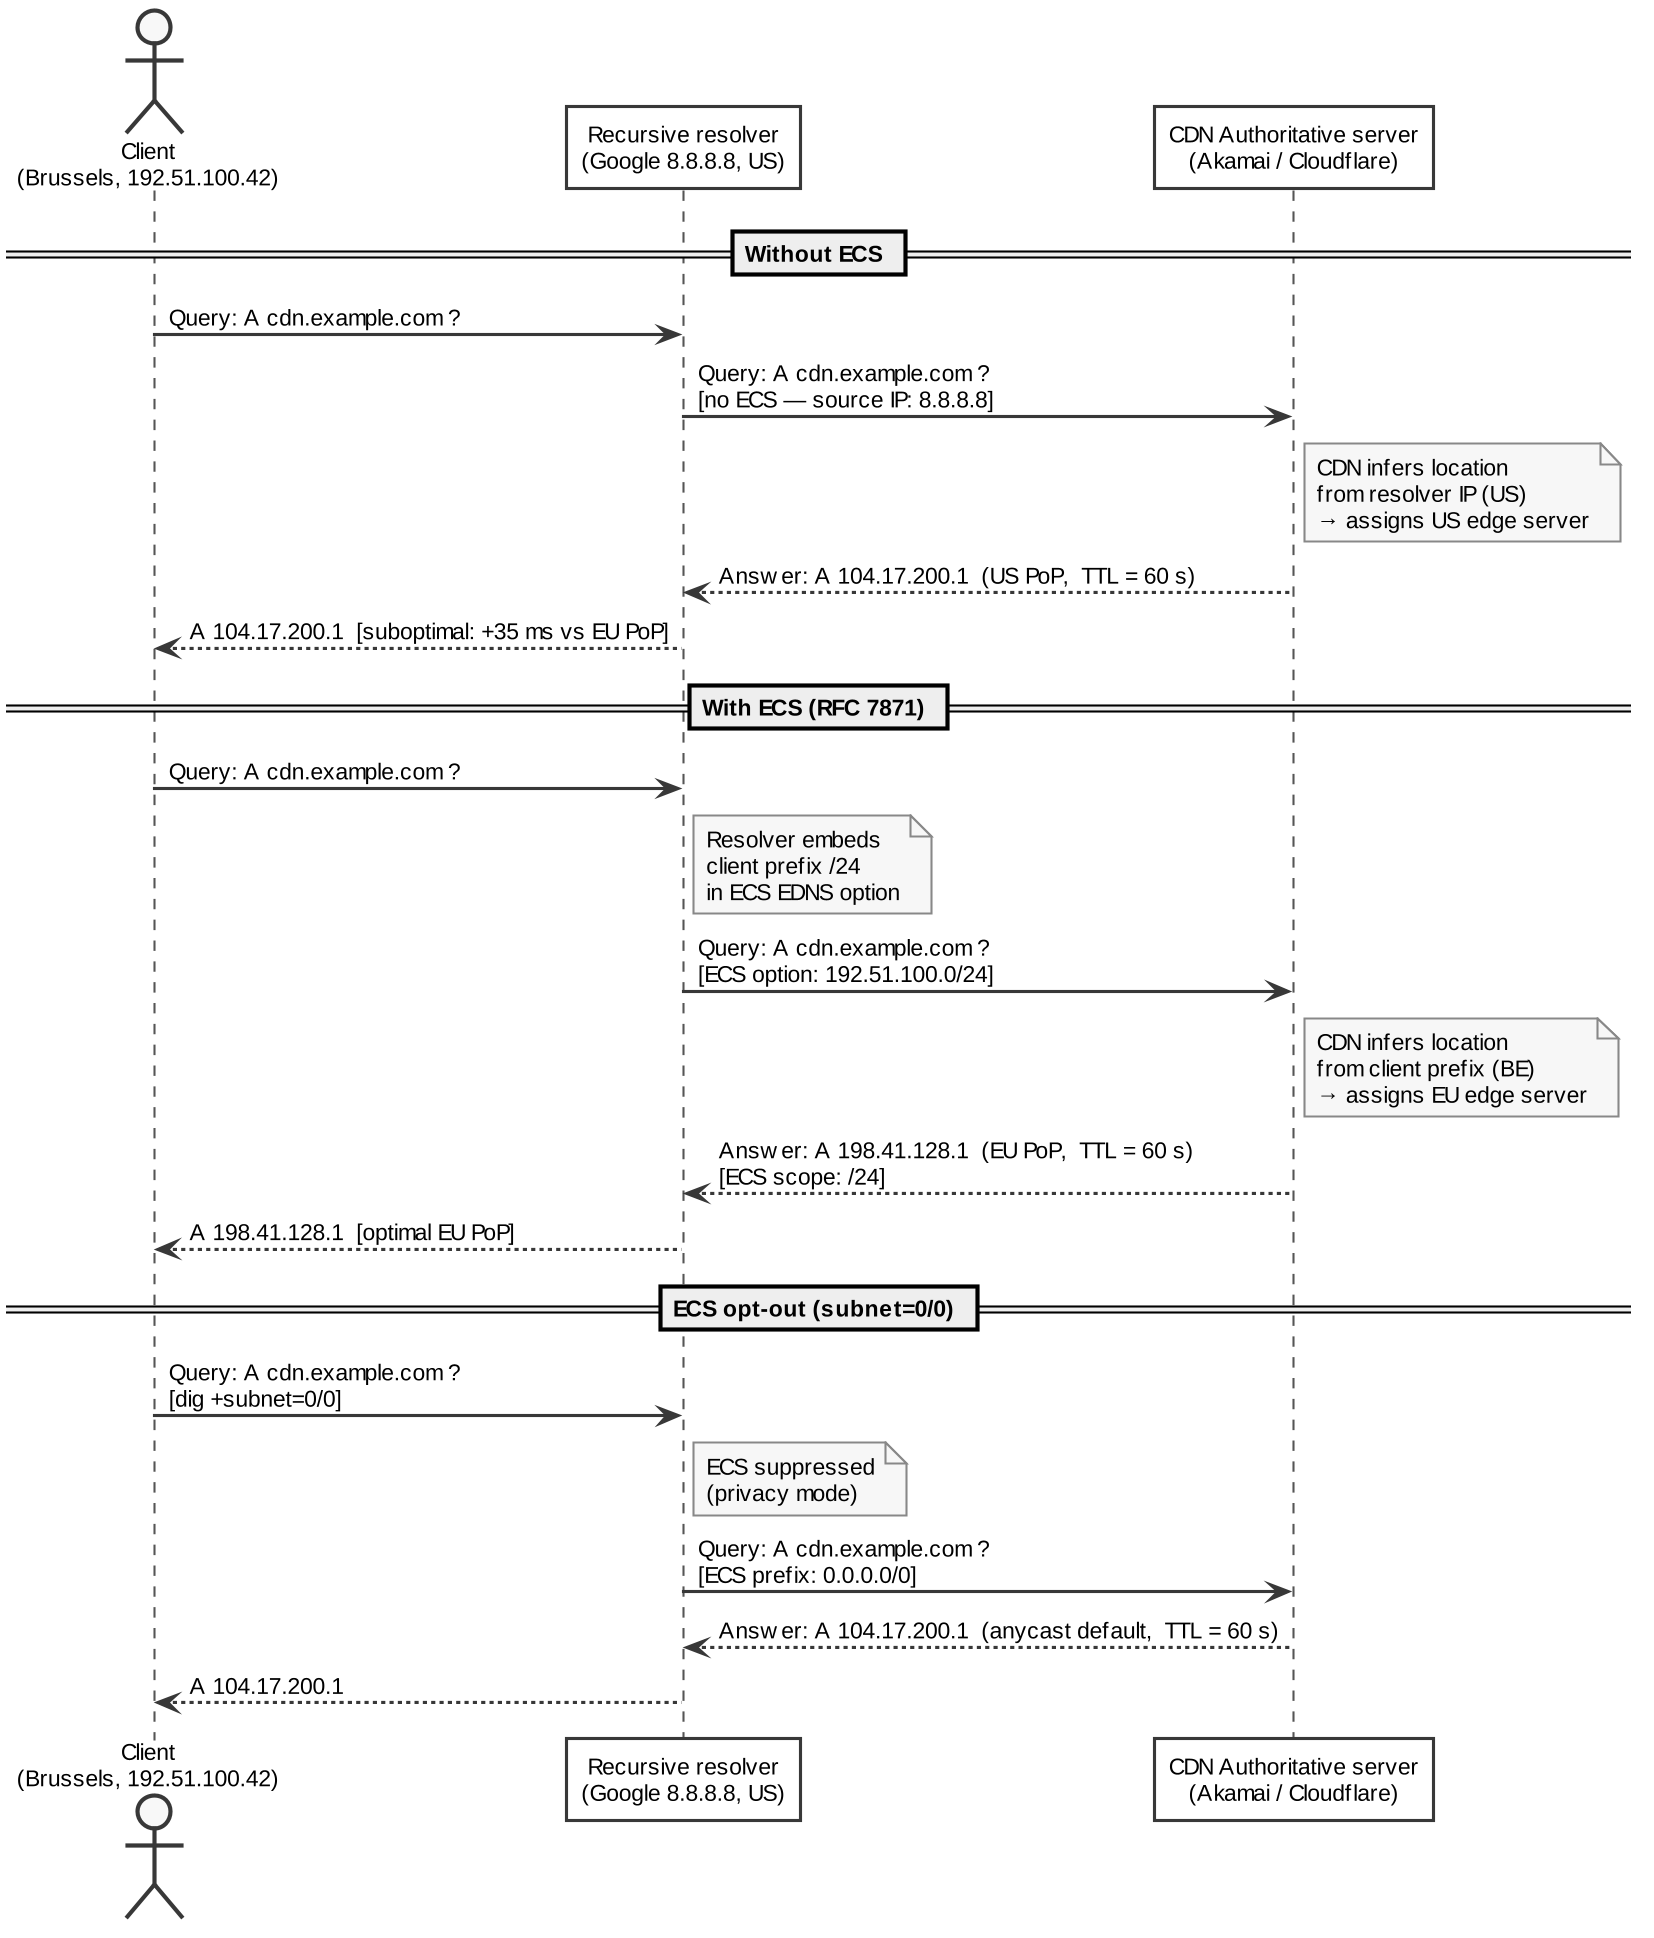
\includegraphics[width=0.90\linewidth]{figures/fig4_ecs_schema.png}
  \caption{Effect of \ac{ECS}~\cite{RFC7871} on \ac{CDN} geographic routing. \textit{Without \ac{ECS}}, the \ac{CDN} authoritative server infers client location from the recursive resolver's \ac{IP} (8.8.8.8, US), assigning a suboptimal US edge server to a Belgian client. \textit{With \ac{ECS}}, the resolver embeds the client's /24 prefix; the \ac{CDN} selects the geographically appropriate EU \ac{PoP}. \textit{\ac{ECS} opt-out} (\texttt{subnet=0/0}) suppresses the prefix entirely, reverting to resolver-\ac{IP}-based routing.}
  \label{fig:ecs_schema}
\end{figure}

\textbf{\ac{DNS} infrastructure centralisation}: Xu~\cite{Xu2023} show that over 90\% of forwarding resolvers are backed by fewer than 5\% of indirect recursive resolvers, and that just 10 \ac{DNS} providers serve 48.5\% of all g\ac{TLD} domain names. This centralisation creates a methodological choice between two complementary approaches, each with distinct trade-offs.

Using the probe's default resolver reflects the experience of real end-users: queries traverse the full recursive resolution chain, including the \ac{ISP} resolver's cache and any \ac{ECS} forwarding behaviour. This approach is appropriate for studying \ac{DNS} as users actually encounter it. Its limitation is that geographic diversity of probes may be partially unreal: two probes from different continents may share the same upstream recursive resolver, making their responses indistinguishable regardless of probe location.

Querying authoritative servers directly involves targeting the authoritative name server’s \ac{IP} and explicitly clearing the \ac{RD} bit, which effectively bypasses the recursive resolver layer. This approach ensures that each probe’s query hits the authoritative infrastructure from its own native \ac{IP} address, allowing us to cleanly isolate the geographic routing signal. A key trade-off, however, is that these metrics do not reflect the actual end-user experience mediated by the recursive resolver chain. The RIPE Atlas platform natively accommodates both of these operational approaches.

This thesis uses direct authoritative queries for Q1–Q3, where the goal is to characterise how the authoritative infrastructure responds to different geographic origins, and three major public resolvers (Cloudflare 1.1.1.1, Google 8.8.8.8, and Quad9 9.9.9.9) for Q4, where the goal is to compare resolver-induced differences in returned responses. The probe's local \ac{ISP} resolver was initially planned as a fourth condition but was abandoned: the RIPE Atlas API rejects the combination of an explicit target IP and \texttt{use\_probe\_resolver}: true, and probe inspection revealed that a large fraction of RIPE Atlas probes forward their local resolver to loopback addresses or directly to public resolvers, making the \ac{ISP} condition structurally indistinguishable from the public resolver conditions.

\section{Domain Ranking Lists}
\label{sec:2.6}

Studies of \ac{DNS} behaviour at scale require a reproducible domain corpus. Le Pochat~\cite{LePochat2019} evaluate four freely available ranking lists — Alexa, Cisco Umbrella, Majestic, and Quantcast — and find they agree on only 70,000 of a combined 2.82 million unique domains (24–33\% rank-biased overlap). Alexa’s 2018 methodology change caused 50\% daily list turnover, making longitudinal studies unreliable; Amazon subsequently shut down the Alexa ranking service entirely on 1 May 2022, making it unavailable for any ongoing research. Cisco Umbrella contains 51\% non-web entries (EC2 hostnames, typos). Majestic contains 2,162 documented malicious domains. All four lists are trivially manipulable: a single \ac{HTTP} request from an Alexa browser extension user can lift a domain to rank 28,798. Table~\ref{tab:ranking_lists} compares the main properties.

\begin{table}[tp]
\centering
\small
\begin{tabularx}{\linewidth}{p{2.2cm} X X X X}
\toprule
\textbf{Property} & \textbf{Alexa} \newline \textit{(discontinued 2022)} & \textbf{Cisco Umbrella} & \textbf{Majestic} & \textbf{Tranco} \\
\midrule
Data source  & Browser extension & \ac{DNS} queries to OpenDNS & Web crawl backlinks & Multi-source aggregation \\
Daily change rate & $\approx$50\,\% (post-2018) & $\approx$10\,\% & $\approx$1\,\% & $\approx$0.6\,\% \\
Manipulation effort & 1 \ac{HTTP} request & 1 \ac{DNS} query injection & Few backlinks & 4$\times$ vs single-source \\
Non-domain entries & Low & $\approx$51\,\% & Low & Filtered \\
Malicious domains & Some & Some & 2\,162 documented & Filtered \\
Reproducibility   & Daily overwrite & Daily overwrite & Daily overwrite & Stable permalink \\
\bottomrule
\end{tabularx}
\caption{Comparison of domain ranking lists. Tranco is the only list designed for research reproducibility and manipulation resistance~\cite{LePochat2019}.}
\label{tab:ranking_lists}
\end{table}

\textbf{Tranco}~\cite{LePochat2019} combines multiple ranking lists over a 30-day rolling window through the Borda count method. This aggregation yields a highly stable corpus with a minimal 0.6\% daily churn rate, while requiring a quadrupled adversarial effort across multiple lists to manipulate rankings. Furthermore, the framework ensures reproducibility by offering permanent, stable archived links. For the scope of this thesis, such stability guarantees that an identical set of domains is evaluated across all 128 daily campaigns, which is essential for conducting a robust temporal comparison.

\section{Synthesis and Research Positioning}
\label{sec:2.7}

The preceding review reveals a clear gap at the intersection of OpenINTEL’s temporal depth and RIPE Atlas’s spatial diversity. OpenINTEL provides daily, \ac{TLD}-wide \ac{DNS} measurement since 2015 but from a single Dutch vantage point: geographic variation is invisible. Existing RIPE Atlas \ac{DNS} studies are predominantly single-campaign, domain-limited case studies (a few hundred domains, one time point): Bortzmeyer~\cite{Bortzmeyer2013} studies a single anycast server; Finnegan~\cite{Finnegan2018} measures one resolver with 500 probes at a single instant; Hours~\cite{Hours2016} targets a handful of \ac{CDN} providers in one campaign; Koch~\cite{Koch2021} analyses root server anycast at one point in time. To date, no research has systematically quantified the exact fraction of popular domains returning geographically differentiated \ac{DNS} responses, nor have studies tracked the underlying driving mechanisms and their monthly evolution. Table~\ref{tab:gap_analysis} formalizes this academic positioning.

\begin{table}[tp]
\centering
\small
\begin{tabularx}{\linewidth}{p{2.8cm} p{3.5cm} p{3.8cm} X}
\toprule
\textbf{Dimension} & \textbf{OpenINTEL-based studies}~\cite{vanRijswijk2016} & \textbf{Existing RIPE Atlas studies}~\cite{Bortzmeyer2013,Finnegan2018,Hours2016,Koch2021} & \textbf{This thesis} \\
\midrule
Domain coverage  & Full \ac{TLD} zone files & Experimenter-defined (per study) & Tranco Top-250 (stable, reproducible) \\
Geographic vantage    & Single point (Netherlands) & $\approx$12\,900 probes, 178 countries & Multi-continent stratification \\
Temporal depth & Daily since March 2015 & Single campaigns & 127-day repeated campaigns \\
Anycast tracking       & Not applicable & Case studies (d.nic.fr, UncensoredDNS) & Systematic across corpus \\
Resolver control   & Fixed central resolver & Local probe resolver (default) & Direct authoritative query \\
\bottomrule
\end{tabularx}
\caption{Positioning of this thesis relative to existing \ac{DNS} measurement infrastructure across five dimensions.
All three columns represent measurement studies; Each row identifies a gap that this work explicitly addresses.}
\label{tab:gap_analysis}
\end{table}

Three critical gaps in the existing literature form the core motivation for this thesis:

\begin{itemize}
\item \textbf{Limitation 1: Absence of population-scale \ac{DNS} characterization}. Prior literature consists largely of isolated anycast case studies (\cite{Bortzmeyer2013,Finnegan2018}) and targeted \ac{CDN} routing analyses (\cite{Hours2016,Li2025}) that focus on a single service or domain at a time. Consequently, the research landscape lacks a comprehensive measurement showing what percentage of the popular-domain ecosystem exhibits geographic differentiation, as well as which mechanisms dominate at scale.

\item \textbf{Limitation 2: Resolver centralization obscuring vantage-point diversity}. Relying on local probe resolvers often introduces an artificial layer of geographic diversity that ultimately vanishes at the resolution layer. This occurs because nearly 90\% of forwarding resolvers consolidate into a mere 5\% of recursive resolvers\cite{Xu2023}. While direct authoritative querying serves as the necessary remedy to bypass this bottleneck, none of the current case studies explicitly document this approach as a core architectural design choice.

\item \textbf{Limitation 3: Lack of temporal dynamics in snapshot studies}. As acknowledged by Koch~\cite{Koch2021} and Bortzmeyer ~\cite{Bortzmeyer2013}, \ac{BGP} routing policies and \ac{CDN} anycast catchments are inherently volatile, changing continuously as operators deploy new \ac{PoPs} or restructure peering agreements. Capturing the true stability of geographic \ac{DNS} response differentiation therefore requires a long campaign rather than a single-snapshot measurement.
\end{itemize}

This thesis addresses all three gaps by deploying a measurement system that queries the Tranco Top-250 directly at authoritative servers from $\approx$200 geographically stratified RIPE Atlas probes, repeated daily over 127 days, with \ac{NSID}-based anycast instance tracking and results archived in Parquet following \ac{FAIR} data principles.
\chapter{Method}
\label{ch:method}

\section{Overview}
\label{sec:3.1}

\subsection{Methodological Objective}
\label{subsec:3.1.1}

The global methodological objective of this thesis is to capture the geographic and temporal diversity of \ac{DNS} responses for a representative corpus of popular domains, using geographically distributed active measurements, in a manner that is reproducible, ethically sound, and practically feasible within the available resource budget. The system must answer four empirical research questions:

\begin{itemize}
  \item \textbf{Q1}: What proportion of Tranco top-ranked domains return geographically differentiated \ac{DNS} responses, and what infrastructure mechanisms explain the differentiation?
  \item \textbf{Q2}: What is the temporal stability of \ac{DNS} responses for popular domains at day, week, and month timescales?
  \item \textbf{Q3}: Do the geographic biases of the RIPE Atlas probe distribution significantly limit the ability to observe geographic \ac{DNS} variation?
  \item \textbf{Q4}: What is the measurable impact of resolver type --- local \ac{ISP} resolver versus public \ac{DNS} service --- on the \ac{DNS} responses observed?
\end{itemize}

\subsection{System Architecture}
\label{subsec:3.1.2}

The measurement system is organised in five sequential stages, inspired by the architecture of OpenINTEL \cite{vanRijswijk2016} but adapted to the constraints and capabilities of the RIPE Atlas platform:

\begin{enumerate}
  \item \textbf{Domain corpus preparation}: Retrieval and filtering of the Tranco Top 250 domain list.
  \item \textbf{Measurement scheduling}: Configuration and deployment of RIPE Atlas \ac{DNS} measurement campaigns.
  \item \textbf{Data collection}: Automated daily retrieval of measurement results via the RIPE Atlas REST API.
  \item \textbf{Storage and preprocessing}: Parsing, validation, and archival in Parquet format.
  \item \textbf{Analysis}: Quantitative analysis addressing Q1--Q4.
\end{enumerate}

The key design trade-off throughout is the three-way tension between domain coverage (how many domains are measured), geographic coverage (how many geographically distributed probes), and temporal resolution (measurement frequency), all bounded by the finite RIPE Atlas credit budget. The system is fully configurable via \texttt{--max-domains} and \texttt{--total-probes} parameters; the main phase operating point is 250 domains and 200 probes, consuming approximately 500,000 credits per day (250 domains $\times$ 200 probes $\times$ 10 credits per measurement).

\begin{table}[H]
\centering
\small
\begin{tabular}{c l l}
\toprule
\textbf{Step} & \textbf{Stage} & \textbf{Output} \\
\midrule
1 & Domain corpus preparation (\texttt{fetch\_tranco.py})         & \texttt{tranco\_corpus.csv} \\
2 & Measurement scheduling (\texttt{create\_ripe\_measurements.py}) & \texttt{measurements.json} \\
3 & Data collection (\texttt{fetch\_ripe\_atlas.py})               & \texttt{data/raw/msm\_*.json} \\
4 & Parsing \& storage (\texttt{parse\_dns\_results.py})           & \texttt{dns\_results*.parquet} \\
5 & Analysis (\texttt{analyse\_dns.py})                            & Reports \& figures \\
\bottomrule
\end{tabular}
\caption{Five-stage pipeline architecture. Steps 1--2 are run once at campaign initialisation; steps 3--4 run daily; step 5 runs weekly.}
\label{tab:pipeline_stages}
\end{table}

\subsection{Infrastructure}
\label{subsec:3.1.3}

The entire pipeline runs as a Docker container on a Raspberry Pi 5 (ARM64 architecture), operating continuously and autonomously. This choice reflects the need for a low-cost, always-on measurement platform that can sustain a 50-day measurement campaign without manual intervention.

The container image is based on \texttt{python:3.11-slim-bookworm} and is compiled natively for the ARM64 architecture, ensuring full compatibility with the Raspberry Pi 5 hardware. The image contains only the dependencies required for the pipeline (dnspython, pandas, pyarrow, scipy, matplotlib, rclone), keeping its footprint under 1 GB.

Data persistence is managed through Docker named volumes, which survive container restarts and image updates. Every day, our system automatically sends a copy of the results to cloud storage using rclone, targeting Google Drive as the remote backup destination.

The pipeline is orchestrated by a cron daemon running inside the container, with the following schedule (all times UTC):

\begin{table}[H]
\centering
\small
\begin{tabular}{l l l}
\toprule
\textbf{Time (UTC)} & \textbf{Day} & \textbf{Action} \\
\midrule
10:00 & Daily & Fetch RIPE Atlas results + Parquet parsing \\
11:00 & Daily & Cloud sync (Parquet + raw JSON $\rightarrow$ Google Drive) \\
12:00 & Sunday & Q1--Q4 analysis + figure generation \\
13:00 & Sunday & Cloud sync (reports + figures $\rightarrow$ Google Drive) \\
04:00 & 1st of month & Log rotation \\
\bottomrule
\end{tabular}
\end{table}

The weekly Tranco list refresh is intentionally disabled during the active measurement period. Keeping the domain corpus fixed throughout the campaign is required for the validity of the Q2 temporal stability analysis: if domains entered or left the measurement set mid-campaign, observed response changes could not be distinguished from corpus changes. The corpus will be refreshed after the measurement period concludes.

The pipeline source code is available at \url{xxx} (\hl{\textit{To be completed}}). The five core scripts (\texttt{fetch\_tranco.py}, \texttt{create\_ripe\_measurements.py}, \texttt{fetch\_ripe\_atlas.py}, \texttt{parse\_dns\_results.py} and \texttt{analyse\_dns.py}) are introduced as they appear in the pipeline, alongside \texttt{pipeline.py}, which acts as the top-level orchestrator and is invoked by the cron scheduler.

\section{Domain Corpus Selection}
\label{sec:3.2}

\subsection{Tranco List Configuration}
\label{subsec:3.2.1}

The domain corpus is the Tranco Top 250 list, retrieved via the Tranco API at \url{https://tranco-list.eu}. The choice of Tranco over commercial ranking lists (Alexa — discontinued May 2022 —, Cisco Umbrella, Majestic) is motivated in Chapter 2 (Section~\ref{sec:2.6}) and rests on three properties established by Le Pochat~\cite{LePochat2019}: stability (0.6\% daily change versus approximately 50\% for post-2018 Alexa), manipulation resistance (quadrupled manipulation effort relative to single-source lists), and archivability (each generated list is assigned a unique identifier retrievable indefinitely via permalink).

The \texttt{fetch\_tranco.py} script retrieves the most recent available list, falling back up to seven days if the current day's list has not yet been published. The exact Tranco list identifier and generation date are recorded in \texttt{tranco\_meta.json} alongside the corpus, ensuring full reproducibility.

The list is retrieved once at the start of the measurement campaign and kept fixed for its entire duration. Although Tranco provides a stable list, any mid-campaign change to the measured domain set would conflate \ac{DNS} response variation with corpus variation, making it impossible to distinguish true temporal instability (Q2) from artefacts of domain rotation. The Tranco list identifier and retrieval date are recorded in \texttt{tranco\_meta.json} to allow exact reproduction of the corpus by any future researcher.

\subsection{Domain Corpus Size}
\label{subsec:3.2.2}

The measurement campaign was conducted in two successive phases, each driven by the available RIPE Atlas credit balance:

\textbf{Pilot phase (1--10 April 2026)}: The corpus was limited to the top 100 domains with 50 probes, consuming approximately 50,000 credits per day. This phase served to validate the full pipeline end-to-end --- probe selection, measurement creation, daily fetch, parsing, and cloud synchronisation --- before committing to a larger credit budget.

\textbf{Main phase (from 11 April 2026)}: Following validation and the allocation of additional RIPE Atlas credits (30,000,000 total), the corpus was extended to 250 domains with 200 probes, consuming approximately 500,000 credits per day. At this rate, the remaining campaign period of approximately 50 days consumes 25,000,000 credits, well within the available balance.

The choice of 250 domains reflects a trade-off between two competing constraints:

\textbf{Representativeness}: The Tranco Top 250 is a great way to get a sense of the big players in the global \ac{CDN}-backed services market. It’s not just about the top dogs, though - it also shines a light on some of the smaller, second-tier platforms that are still worth paying attention to. Studies by Calder~\cite{Calder2015} and Wang~\cite{Wang2018} confirm that \ac{CDN} routing diversity is most pronounced in the highest-traffic domains, but measurable geographic variation extends into the broader popular-domain tier, motivating the extension beyond the pilot corpus.

\textbf{Feasibility}: At 200 probes per measurement, the Top 250 corpus consumes 500,000 credits per day --- sustainable over the 50-day main phase within the available credit allocation of 30,000,000 credits.

The pipeline exposes \texttt{--max-domains} and \texttt{--total-probes} parameters, so the corpus can be extended to a larger Tranco slice without any further modification.

\subsection{Domain Filtering and Validation}
\label{subsec:3.2.3}

Before the measurement campaign begins, each domain in the Tranco list is pre-validated by 

\texttt{fetch\_tranco.py} in two steps:

\textbf{Technical validity}: A \ac{DNS} \ac{A} record query is issued against Google Public \ac{DNS} (8.8.8.8) and Cloudflare \ac{DNS} (1.1.1.1) as reference resolvers. Domains returning \texttt{NXDOMAIN} or \texttt{SERVFAIL} are excluded. Applied to the Tranco Top 10,000 list from which the campaign corpus is drawn, this step yielded 8,365 valid domains --- a filtering rate of approximately 16\%, higher than the 5--6\% reported by Le Pochat~\cite{LePochat2019}, which may reflect the broader scope of the list and the inclusion of parked or inactive domains in lower-ranked positions.

\textbf{Authoritative server pre-resolution}: The authoritative name servers for each domain are identified by resolving the domain's \ac{NS} records from the same reference resolvers. This pre-resolution step maps each domain to its authoritative server set. The resulting corpus is saved as \texttt{tranco\_corpus.csv} with fields \texttt{rank}, \texttt{domain}, and \texttt{ns} (pipe-separated list of authoritative name-server hostnames). Domains for which the \ac{NS} \ac{IP} address could not be resolved at measurement time are skipped. In practice, 2 of the top-250 domains were excluded on this basis, yielding 248 active RIPE Atlas measurements for the main campaign.

\section{RIPE Atlas Measurement Configuration}
\label{sec:3.3}

\subsection{Probe Selection}
\label{subsec:3.3.1}

Probe selection is implemented in \texttt{create\_ripe\_measurements.py} and follows the filtering protocol recommended by Bajpai et al.~\cite{Bajpai2017}. Geographic distribution across zones is delegated to RIPE Atlas. The selection proceeds in three steps.

\textbf{Step 1 --- System tag filtering}: All probes must satisfy the following RIPE Atlas system tags:

\begin{itemize}
  \item \texttt{system-ipv4-works}: \ac{IPv4} connectivity verified by built-in platform measurements.
  \item \texttt{system-resolves-a-correctly}: The probe's local resolver returns correct \ac{A} records, filtering out probes whose resolver intercepts or misroutes external queries~\cite{Boswell2024}.

\end{itemize}

For hardware probes, version v3 or later is required. Holterbach~\cite{Holterbach2015} show that hardware v1 and v2 probes experience timing precision degradation under concurrent measurement load (up to +7.7\,ms at the 95th percentile), while v3 probes experience negligible degradation (+0.06\,ms); software probes are not subject to this hardware constraint.

\textbf{Step 2 --- Geographic distribution}: To compensate for RIPE Atlas's documented geographic concentration (91\% of dual-stacked probes in the "\ac{RIPE NCC}" and "\ac{ARIN}" regions~\cite{Bajpai2017}), probe allocation targets an inverse-weighted over-representation of under-represented regions. For the current campaign, geographic distribution is delegated to RIPE Atlas using five built-in geographic zones with the following allocation:

\begin{table}[H]
\centering
\small
\begin{tabular}{l r}
\toprule
\textbf{RIPE Atlas zone} & \textbf{Allocation (200 probes)} \\
\midrule
West           & 60 (30\%) \\
North-Central  & 48 (24\%) \\
South-East     & 40 (20\%) \\
North-East     & 32 (16\%) \\
South-Central  & 20 (10\%) \\
\textbf{Total} & \textbf{200 (100\%)} \\
\bottomrule
\end{tabular}
\end{table}

\begin{figure}[H]
\centering
\includegraphics[width=0.85\linewidth]{figures/ripe_atlas_zones_map.png}
\caption{Geographic coverage of the five RIPE Atlas probe zones used for probe allocation. Source:~\cite{RIPEAtlasDocs2026}.}
\label{fig:ripe_atlas_zones}
\end{figure}

The resulting continent-level distribution is reported in Table~\ref{tab:4.2}. For future campaigns, the pipeline implements a continent-level stratification (Step 3) designed to achieve the following targets:

\begin{table}[H]
\centering
\small
\begin{tabular}{l l l l l}
\toprule
\textbf{Region} & \textbf{Atlas distribution} & \textbf{Pilot (50 probes)} & \textbf{Main (200 probes)} & \textbf{Target \%} \\
\midrule
Europe        & \textasciitilde{}40\% & 15  & 60  & 30\% \\
North America & \textasciitilde{}28\% & 12  & 50  & 25\% \\
Asia-Pacific  & \textasciitilde{}16\% & 10  & 40  & 20\% \\
South America & \textasciitilde{}8\%  &  5  & 20  & 10\% \\
Africa        & \textasciitilde{}5\%  &  5  & 20  & 10\% \\
Oceania       & \textasciitilde{}3\%  &  3  & 10  &  5\% \\
\textbf{Total} & \textbf{100\%} & \textbf{50} & \textbf{200} & \textbf{100\%} \\
\bottomrule
\end{tabular}
\end{table}

These proportions preserve the relative weighting from prior work~\cite{Bajpai2017} while scaling to the target probe count. The probe count is configurable via \texttt{--total-probes}.

\textbf{Step 3 --- Country and \ac{AS} diversity}: Within each continental stratum, the pipeline implements a three-round algorithm to maximise both country coverage and \ac{AS} diversity:

\begin{itemize}
  \item \textbf{Round 1}: One probe per country, prioritising countries not geographically assimilated by a larger neighbour. Micro-states and dependencies (Luxembourg, Monaco, San Marino, Liechtenstein, Andorra, Vatican, Gibraltar, etc.) are de-prioritised, as their \ac{DNS} infrastructure typically routes through the same \ac{CDN} \ac{PoPs} as their larger neighbours.
  \item \textbf{Round 2}: One probe per de-prioritised country, if the continental quota has not yet been reached.
  \item \textbf{Round 3}: Additional probes per country (preferring a different \ac{AS} each time) until the quota is filled.
\end{itemize}

Within each round, the probe selected for a given country is the one with the highest hardware version that introduces a new \ac{AS} not yet represented in the selected set. The selected probe set is saved as \texttt{selected\_probes\_<date>.json} for full reproducibility. This algorithm is fully implemented in the pipeline and will be activated for future campaigns, replacing the zone-based assignment used for the current campaign.

\subsection{Primary Campaign: Direct Authoritative DNS Queries}
\label{subsec:3.3.2}

The primary measurement campaign queries authoritative name servers directly, bypassing recursive resolvers. As discussed in Chapter 2 (Section~\ref{sec:2.5}), two complementary approaches are possible: using the probe's default resolver (which reflects real user experience) or querying the authoritative server directly (which isolates the geographic routing signal). For Q1--Q3, the direct authoritative approach is chosen for two reasons:

\begin{enumerate}
  \item \textbf{Resolver centralization} \cite{Xu2023}: Over 90\% of forwarding resolvers are backed by fewer than 5\% of indirect recursive resolvers. Querying through probe resolvers would collapse the geographic diversity of probe vantage points into a small number of centralised resolution paths, making geographic \ac{DNS} variation invisible.
  \item \textbf{Cache state divergence}: Probes using local resolvers have heterogeneous cache states, introducing variation that mimics geographic routing differences but is actually an artefact of cache timing. Direct authoritative queries bypass resolver caches entirely.
\end{enumerate}

The default resolver approach is used for Q4 (Section~\ref{subsec:3.3.3}), where the research question is precisely about the impact of resolver choice on end-user experience.

For each domain in the corpus, the primary authoritative name server identified during pre-resolution is used as the measurement target. The RIPE Atlas \ac{DNS} measurement is configured as follows:


\begin{lstlisting}[style=json]
{
  "type": "dns",
  "af": 4,
  "target": "<authoritative_ns_ip>",
  "query_type": "A",
  "query_class": "IN",
  "query_argument": "<domain>",
  "use_probe_resolver": false,
  "set_rd_bit": false,
  "set_nsid_bit": true,
  "set_do_bit": false,
  "set_cd_bit": false,
  "protocol": "UDP",
  "udp_payload_size": 1024,
  "include_abuf": true,
  "retry": 2,
  "timeout": 5000,
  "is_oneoff": false,
  "interval": 86400,
  "description": "DNS geo-diversity - auth - <domain> - <YYYY-MM-DD>"
}

\end{lstlisting}

Table~\ref{tab:msm_params} describes each parameter and its justification.

Full API documentation is available in~\cite{RIPEAtlasDocs2026}.

\begin{table}[H]
\centering
\small
\begin{tabularx}{\linewidth}{l l X}
\toprule
\textbf{Parameter} & \textbf{Value} & \textbf{Justification} \\
\midrule
\texttt{type} & \texttt{"dns"} & RIPE Atlas measurement type for \ac{DNS} queries. \\
\texttt{af} & \texttt{4} & \ac{IPv4} address family; probes resolve the target using \ac{IPv4}. \\
\texttt{target} & \textit{ns\_ip} & \ac{IP} address of the authoritative name server identified during pre-resolution; queries bypass recursive resolvers entirely. \\
\texttt{query\_type} & \texttt{"A"} & Requests \ac{IPv4} address records, which are the primary indicator of \ac{CDN} geographic routing. \\
\texttt{query\_class} & \texttt{"IN"} & Internet class; the only class used in practice for public \ac{DNS}. \\
\texttt{query\_argument} & \textit{domain} & The domain name being queried. \\
\texttt{use\_probe\_resolver} & \texttt{false} & Disables routing through the probe's local resolver; queries are sent directly to the authoritative server. \\
\texttt{set\_rd\_bit} & \texttt{false} & \ac{RD} bit unset; the authoritative server is queried directly and must not recurse. \\
\texttt{set\_nsid\_bit} & \texttt{true} & Requests the \ac{NSID} option~\cite{RFC5001}; the authoritative server's response identifies the physical anycast instance that answered, enabling anycast routing analysis~\cite{Bortzmeyer2013,Finnegan2018}. \\
\texttt{set\_do\_bit} & \texttt{false} & \ac{DNSSEC} OK bit unset; \ac{DNSSEC} validation is not required for \ac{IP} address collection and would increase response size without benefit. \\
\texttt{set\_cd\_bit} & \texttt{false} & Checking Disabled bit unset; \ac{DNSSEC} checking is not relevant for direct authoritative queries. \\
\texttt{protocol} & \texttt{"UDP"} & Standard \ac{DNS} transport; UDP is used by default and is sufficient for responses of this size. \\
\texttt{udp\_payload\_size} & \texttt{1024} & EDNS0 buffer size in bytes; set large enough to accommodate the \ac{NSID} option in the response without truncation. \\
\texttt{include\_abuf} & \texttt{true} & Includes the raw \ac{DNS} response packet (base64-encoded), enabling full parsing of all \ac{DNS} sections and OPT record \ac{NSID} decoding~\cite{RFC5001}. \\
\texttt{retry} & \texttt{2} & Number of retransmission attempts on timeout before the result is recorded as no-response. \\
\texttt{timeout} & \texttt{5000} & Per-attempt timeout in milliseconds (5 seconds); consistent with RIPE Atlas defaults for \ac{DNS} measurements. \\
\texttt{is\_oneoff} & \texttt{false} & Configures the measurement as periodic rather than a one-shot query. \\
\texttt{interval} & \texttt{86400} & Repetition interval in seconds (24 hours); provides the daily temporal resolution needed to detect \ac{DNS} response changes within the credit budget. \\
\texttt{description} & \textit{see value} & Human-readable label in the RIPE Atlas dashboard, including the domain name and creation date for traceability. \\
\bottomrule
\end{tabularx}
\caption{RIPE Atlas DNS measurement parameters for the primary Q1--Q3 campaign.}
\label{tab:msm_params}
\end{table}

\subsection{Supplementary Campaign for Q4: Resolver Comparison}
\label{subsec:3.3.3}

To address Q4, a supplementary one-off measurement campaign is conducted on the full 250-domain corpus using the same 200 probes as Q1--Q3. Using the same probe set ensures that any observed inter-resolver divergence is attributable to resolver infrastructure rather than probe geographic differences. This campaign provides three simultaneous resolver observations per domain per probe:

\begin{table}[H]
\centering
\small
\begin{tabular}{l l l}
\toprule
\textbf{Campaign label} & \textbf{Target IP} & \textbf{Resolver} \\
\midrule
\texttt{google} & 8.8.8.8 & Google Public \ac{DNS} \\
\texttt{cloudflare} & 1.1.1.1 & Cloudflare \ac{DNS} \\
\texttt{quad9} & 9.9.9.9 & Quad9 \\
\bottomrule
\end{tabular}
\end{table}

The Q4 campaign uses \texttt{set\_rd\_bit: true} and a \ac{UDP} payload of 4096 bytes, appropriate for recursive resolver queries. Measurements are configured as one-off (\texttt{is\_oneoff: true}) to avoid continuous credit consumption. A fourth configuration targeting the probe's local \ac{ISP} resolver via \texttt{use\_probe\_resolver: true} was planned but abandoned: the RIPE Atlas API rejects the combination of a target \ac{IP} and \texttt{use\_probe\_resolver: true}, and empirical testing of the probe's \texttt{/etc/resolv.conf} entry showed that a large fraction of probes point to loopback addresses or directly to public resolvers, making the \ac{ISP} condition indistinguishable from the public-resolver conditions.

This three-way comparison tests whether the choice of public recursive resolver affects the \ac{CDN}-assigned \ac{IP} addresses observed from each geographic vantage point, and quantifies the contribution of resolver-level infrastructure (anycast routing, \ac{ECS} policy) to overall \ac{DNS} response variability.

\subsection{Credit Budget}
\label{subsec:3.3.4}

The RIPE Atlas credit consumption is estimated as follows (10 credits per probe per measurement instance):

\begin{table}[H]
\centering
\small
\begin{tabular}{l l l l l}
\toprule
\textbf{Phase} & \textbf{Domains} & \textbf{Probes} & \textbf{Duration} & \textbf{Credits} \\
\midrule
Pilot — primary (direct auth)       & 100 &  50 & 10 days  & $\approx$500,000 \\
Pilot — Q4 resolver comparison      &  50 &  50 & once     & $\approx$100,000 \\
Main — primary (direct auth)        & 250 & 200 & 50 days  & $\approx$25,000,000 \\
Main — Q4 resolver comparison       & 250 & 200 & once     & $\approx$2,000,000 \\
\textbf{Total campaign}             &     &     &          & $\approx$\textbf{27,600,000} \\
\bottomrule
\end{tabular}
\end{table}

One-off DNS measurements consume 20 credits per probe (double the periodic rate), because results are delivered immediately rather than batched. The main Q4 campaign therefore costs $750 \times 200 \times 20 = 3{,}000{,}000$ credits, spread over three days due to RIPE Atlas's rolling 24-hour credit limit of 1,000,000 credits. The total estimated consumption of approximately 28,600,000 credits remains within the initial balance of 30,000,000 credits, leaving a margin of approximately 1,400,000 credits. The credit budget is monitored by the log output of \texttt{create\_ripe\_measurements.py}, which prints the estimated daily and total consumption before any measurements are created.

\section{Data Collection and Processing}
\label{sec:3.4}

\subsection{Daily Collection Pipeline}
\label{subsec:3.4.1}

Measurement results are collected from the RIPE Atlas REST API by \texttt{fetch\_ripe\_atlas.py} on a daily schedule at 10:00 UTC, retrieving results for the previous calendar day. The script reads the measurement plan from \texttt{measurements.json} (produced by \texttt{create\_ripe\_measurements.py}) and iterates over all active measurement identifiers.

The collection is fully paginated, following RIPE Atlas API \texttt{next} links until all results for the time window are retrieved. Error handling includes automatic retry with exponential backoff (up to 5 attempts, base delay 2 seconds, doubling on each retry) and explicit handling of \ac{HTTP} 429 rate-limit responses (waits for the \texttt{Retry-After} header duration before retrying). Failed measurement IDs are recorded in \texttt{fetch\_errors\_<date>.json} for subsequent investigation. And to avoid downloading the same files over and over, it skips the ones it’s already got, unless \texttt{--force} flag is specified to make it redo them anyway.

The raw results are stored in JSON files, which are kept in the data/raw/ folder and named \texttt{data/raw/m\-sm\_<id>\_<date>.json}.

\subsection{Parsing and Field Extraction}
\label{subsec:3.4.2}

Each raw RIPE Atlas \ac{DNS} result is parsed by \texttt{parse\_dns\_results.py}, which extracts the following fields into a structured Parquet record:

\begin{table}[H]
\centering
\small
\begin{tabular}{l l l}
\toprule
\textbf{Field} & \textbf{Type} & \textbf{Description} \\
\midrule
\texttt{msm\_id} & int64 & RIPE Atlas measurement ID \\
\texttt{prb\_id} & int32 & RIPE Atlas probe ID \\
\texttt{timestamp} & int64 & Actual measurement time (Unix epoch) \\
\texttt{date} & string & ISO date (YYYY-MM-DD) \\
\texttt{country\_code} & string & ISO 3166-1 alpha-2 country code \\
\texttt{asn\_v4} & int32 & Probe \ac{AS} Number \\
\texttt{continent} & string & Continent code (EU/NA/SA/AF/AP/OC) \\
\texttt{query\_domain} & string & Queried domain name \\
\texttt{rcode} & int16 & \ac{DNS} response code (0 = NOERROR) \\
\texttt{answer\_count} & int16 & Number of \ac{A}/\ac{AAAA} records returned \\
\texttt{answer\_ips} & string & Pipe-separated list of returned \ac{IP} addresses \\
\texttt{ttl\_min} & int32 & Minimum \ac{TTL} across answer records \\
\texttt{rt\_ms} & float32 & Response time in milliseconds \\
\texttt{nsid\_str} & string & \ac{NSID} value (ASCII, if returned) \\
\texttt{nsid\_hex} & string & \ac{NSID} value (hex encoding) \\
\texttt{abuf\_size} & int32 & \ac{DNS} response packet size in bytes \\
\texttt{resolver\_ip} & string & Target resolver \ac{IP} (Q4 campaign only) \\
\texttt{use\_probe\_resolver} & bool & True for \ac{ISP} local resolver campaign \\
\bottomrule
\end{tabular}
\end{table}

The \ac{NSID} value is extracted by decoding the raw ABUF binary field: the script walks the \ac{DNS} packet structure to locate the OPT record (type 41) in the Additional section, then parses EDNS0 options to extract option code 3 (\ac{NSID}, ~\cite{RFC5001}).

\subsection{Data Validation}
\label{subsec:3.4.3}

The following validation filters are applied during parsing:

\textbf{RCODE filtering}: Only results with \texttt{rcode = 0} (NOERROR) and \texttt{answer\_count > 0} are used for Q1 and Q2 content analysis. Results with \texttt{rcode != 0} are retained in the Parquet dataset with their specific error codes for reliability and censorship analysis.

\textbf{Deduplication}: The cumulative Parquet file (\texttt{dns\_results.parquet}) is deduplicated on \texttt{(msm\_id, prb\_id, timestamp)} on each daily append to prevent double-counting in case of re-fetch. Here \texttt{timestamp} is the measurement timestamp set by the probe at the moment of the DNS query --- not the fetch time --- so re-fetching the same day's results produces identical tuples and the deduplication correctly discards the duplicates.

\subsection{Storage Architecture}
\label{subsec:3.4.4}

Results are stored in a single-tier Parquet architecture optimised for the analytical query patterns of the analysis phase:

\textbf{Cumulative Parquet file} (\texttt{data/processed/dns\_results.parquet}): All parsed results are appended daily to a single Parquet file using pyarrow with a fixed schema. This file grows at approximately 40--60 MB/month for the primary campaign (250 domains $\times$ 200 probes $\times$ 30 days, after columnar compression with dictionary encoding for repeated string values such as \texttt{country\_code}, \texttt{continent}, and \texttt{answer\_ips}).

\textbf{Daily archives} (\texttt{data/processed/dns\_results\_<date>.parquet}): Individual daily Parquet files are also retained for point-in-time analysis and as a recovery mechanism in case of cumulative file corruption.

\textbf{Raw JSON files} (\texttt{data/raw/msm\_<id>\_<date>.json}): Raw RIPE Atlas JSON results are retained locally for 7 days, then deleted after cloud synchronisation. This rolling window allows re-parsing with an updated schema if needed, while controlling local storage consumption on the Raspberry Pi.

\textbf{Cloud backup}: All Parquet files, daily archives, and reports are synchronised daily to Google Drive via rclone. The rclone configuration is persisted in a Docker named volume, surviving container updates.

\textbf{Storage estimate} for a 50-day campaign (250 domains $\times$ 200 probes):

\begin{table}[H]
\centering
\small
\begin{tabular}{l l l}
\toprule
\textbf{Tier} & \textbf{Volume} & \textbf{Location} \\
\midrule
Raw JSON (7-day rolling) & \textasciitilde{}70 MB & Pi local \\
Cumulative Parquet & \textasciitilde{}80--100 MB & Pi + Google Drive \\
Daily Parquet archives & \textasciitilde{}80--100 MB & Pi + Google Drive \\
Reports and figures & \textasciitilde{}50 MB & Pi + Google Drive \\
\bottomrule
\end{tabular}
\end{table}

\bigskip
\section{Analysis Methods}
\label{sec:3.5}

This section explains how the analyses were done using \texttt{analyse\_dns.py}. This script is listed as step 5 in Table~\ref{tab:pipeline_stages}. It reads the cumulative \texttt{dns\_results.parquet} file and produces reports and figures for each question. The reports are in CSV format and the figures are in PNG format.

\subsection{Statistical Testing Approach}
\label{subsec:3.5.0}

Several analyses in this section compare two independent groups of observations (e.g.\ probes from different geographic regions, or different resolver types). All such comparisons use the Mann-Whitney U test (also known as the Wilcoxon rank-sum test), a non-parametric test that evaluates whether one group tends to produce systematically larger values than the other, without assuming any particular distribution of the data.

The Mann-Whitney U test was chosen instead of a Student's t-test. The t-test is a parametric test that compares the means of two groups under the assumption that the data follow a normal distribution; it is widely used but sensitive to violations of that assumption. Here, two characteristics of the data make the t-test unsuitable. First, the primary response variable --- the number of unique \ac{IP} addresses observed per domain --- is a count variable with a heavily right-skewed distribution: most domains return one or two \ac{IP} addresses, while a small number of \ac{CDN}-heavy domains return many more, violating the normality assumption. Second, the groups being compared are of unequal size, which further reduces the reliability of parametric tests on small samples. The Mann-Whitney U test is robust to both non-normality and unequal group sizes.

The null hypothesis in each case is that the two groups are drawn from the same distribution (i.e.\ no systematic difference). A p-value below 0.05 is used as the significance threshold throughout.

\subsection{Q1 --- Geographic Diversity of DNS Responses}
\label{subsec:3.5.1}

\textbf{Objective}: For each domain in the corpus, determine whether the set of \ac{IP} addresses returned varies systematically by the geographic location of the querying probe.

The study works on two different levels, looking at things from a broad view and a more detailed view. It uses the variety of data from different countries, which was made possible by the stratified selection algorithm (Section~\ref{subsec:3.3.1}).

\textbf{Step 1 --- Continent-level diversity (coarse)}: For each domain and each measurement day, the probe set is partitioned by continent. For each continent, the union of all \ac{IP} addresses returned by probes in that continent is computed. A domain is classified as continent-diverse if at least two continents receive distinct \ac{IP} address sets on the same day. This level of analysis is comparable to prior RIPE Atlas \ac{DNS} studies.

\textbf{Step 2 --- Country-level diversity (fine-grained)}: The same computation is repeated at the country level. A domain is classified as country-diverse if at least two countries receive distinct \ac{IP} address sets on the same day. This finer granularity can reveal intra-continental differentiation --- cases where \ac{DNS} routing differs between countries within the same continent (e.g.\ within Europe, or between Brazil and Argentina in South America) --- which would be invisible at continent level alone.

\textbf{Step 3 --- Aggregate over time}: For each domain, the proportion of measurement days on which geographic differentiation is observed (\texttt{pct\_geo\_diverse}) characterises the consistency of differentiation over the campaign. A domain is considered to have geographic diversity if there's at least one day when differentiation is observed.

\textbf{Step 4 --- \ac{NSID} analysis}: For domains with geographic \ac{IP} variation, the presence of \ac{NSID} values is used to distinguish between anycast instance selection (different \ac{NSID} per region, indicating different anycast \ac{PoP}) and \ac{DNS}-based \ac{CDN} routing (uniform \ac{NSID} with varying \ac{A} records, indicating \ac{CDN} geographic database lookup).

\textbf{Key metrics}:
\begin{itemize}
  \item Proportion of domains exhibiting continent-level geographic diversity
  \item Proportion of domains exhibiting country-level geographic diversity
  \item Proportion of domains exhibiting intra-continental diversity (country-level only)
  \item Distribution of the number of distinct \ac{IP} address sets across countries and continents
  \item Top domains by country-level geographic diversity score
  \item Proportion of geographically diverse domains returning \ac{NSID} values
\end{itemize}

\subsection{Q2 --- Temporal Stability}
\label{subsec:3.5.2}

\textbf{Objective}: Quantify the rate of change of \ac{DNS} responses for each domain over time.

\textbf{Step 1 --- Per-probe change detection}: For each (domain, probe) pair, consecutive daily observations are compared. A change event is recorded when the \texttt{answer\_ips} value differs between two consecutive measurement days.

\textbf{Step 2 --- Change rate computation}: The per-domain change rate is the proportion of observation pairs for which at least one probe observes a change in the \ac{IP} address set. It is computed at three temporal granularities: daily (pairs of consecutive days), weekly (pairs of observations 7 days apart), and monthly (pairs of observations 30 days apart).

\textbf{Step 3 --- Distribution analysis}: The distribution of per-domain change rates is computed across the full corpus, identifying the proportions of fully stable, occasionally changing, and highly volatile domains.

\textbf{Key metrics}:
\begin{itemize}
  \item Distribution of per-domain daily change rates
  \item Proportion of fully stable domains (0\% change rate)
  \item Median change rate across the corpus
  \item Stability breakdown by temporal window (day/week/month)
\end{itemize}

\subsection{Q3 --- Assessment of RIPE Atlas Geographic Bias}
\label{subsec:3.5.3}

\textbf{Objective}: Evaluate whether the geographic concentration of RIPE Atlas probes in Europe and North America significantly limits the ability to observe geographic \ac{DNS} variation, at both continent and country level.

The analysis operates at the same two levels of granularity as Q1, assessing probe bias at both continent and country level. Both sub-analyses use the Mann-Whitney U test described in Section~\ref{subsec:3.5.0}.

\textbf{Continent-level bias}: The probe distribution actually achieved at deployment is compared to the target allocation from Section~\ref{subsec:3.3.1}. For each continent, the coverage rate (proportion of domains observed by at least one probe) and the mean number of unique \ac{IP} addresses observed per domain are computed. The Mann-Whitney U test compares the distribution of unique \ac{IP}s per domain between Europe+North America probes and probes from all other regions. A statistically significant result indicates that the geographic stratification captures meaningfully different \ac{DNS} responses from under-represented regions; a non-significant result would suggest that EU+NA probes alone would have been sufficient.

\textbf{Country-level bias}: The probe selection algorithm (Section~\ref{subsec:3.3.1}) operates in three rounds within each continental stratum. Round~1 assigns one probe per country (country-first strategy); Round~3 adds extra probes per country to fill remaining continental quotas. This naturally produces two categories: single-probe countries (covered exactly once in Round~1, representing marginal geographic coverage) and multi-probe countries (receiving additional probes in Round~3, typically larger or better-connected countries).

The Mann-Whitney U test compares the number of unique \ac{IP} addresses observed per domain from single-probe countries against those from multi-probe countries. A statistically significant result indicates that single-probe (marginal) countries genuinely observe distinct \ac{DNS} responses --- validating the country-first selection strategy and confirming that the extra geographic diversity is not redundant. A non-significant result would suggest that the additional countries covered by Round~1 add breadth without adding observational value.

\textbf{Key metrics}:
\begin{itemize}
  \item Actual probe distribution by continent and by country at deployment
  \item Number of distinct countries with at least one probe
  \item Number of single-probe vs.\ multi-probe countries per continent
  \item Mean unique \ac{IP}s per domain per continent
  \item Mann-Whitney U: EU+NA vs.\ other continents
  \item Mann-Whitney U: single-probe vs.\ multi-probe countries
\end{itemize}

\subsection{Q4 --- Impact of Resolver Choice}
\label{subsec:3.5.4}

\textbf{Objective}: Quantify inter-resolver divergence among three major public \ac{DNS} services (Google 8.8.8.8, Cloudflare 1.1.1.1, Quad9 9.9.9.9) and identify the infrastructure mechanisms responsible.

This analysis uses the supplementary Q4 measurement campaign (Section~\ref{subsec:3.3.3}), which provides three simultaneous observations for 250 domains from the same 200 probes.

\textbf{Step 1 --- Per-resolver statistics}: For each resolver (\texttt{google}, \texttt{cloudflare}, \texttt{quad9}), the following metrics are computed: error rate (proportion of RCODE $\neq$ 0), median \ac{RTT}, mean \ac{RTT}, and mean answer count.

\textbf{Step 2 --- Pairwise divergence analysis}: For each (domain, probe) pair, the \texttt{answer\_ips} returned by each resolver are compared across all three resolver pairs (Google vs.\ Cloudflare, Google vs.\ Quad9, Cloudflare vs.\ Quad9). A divergence event is recorded when the two \ac{IP} sets are completely disjoint. The per-pair divergence rate is the proportion of (domain, probe) tuples showing divergence.

\textbf{Key metrics}:
\begin{itemize}
  \item Error rate and median \ac{RTT} per resolver
  \item Pairwise \ac{IP} divergence rate for all three resolver pairs
\end{itemize}

\bigskip
\section{Ethical Considerations and Reproducibility}
\label{sec:3.6}

\subsection{Ethical Design}
\label{subsec:3.6.1}

The measurement design follows the ethical framework of Kisteleki~\cite{Kisteleki2016} and the principles of the Menlo Report (2012)~\cite{Bailey2012}:

\textbf{Probe host protection}: All query targets are publicly accessible domains from the Tranco Top 250 corpus. Direct authoritative queries for \ac{A} records are indistinguishable from normal client \ac{DNS} traffic.

\textbf{Infrastructure impact}: The measurement frequency (once per domain per day, 200 probes, 250 domains) generates approximately 50,000 queries per day --- negligible compared to OpenINTEL's production campaign of several hundred million queries per day \cite{vanRijswijk2016}.

\textbf{Transparency}: All measurements are tagged with a project description in RIPE Atlas, allowing authoritative server operators to identify the measurement source. The measurement plan (\texttt{measure\-ments.json}) records all active measurement IDs.

\subsection{Scientific Reproducibility}
\label{subsec:3.6.2}

\textbf{Fixed domain corpus}: The Tranco list identifier recorded in \texttt{tranco\_meta.json} for each measurement week enables exact reproduction of the domain corpus.

\textbf{Measurement traceability}: All RIPE Atlas measurement IDs are recorded in \texttt{measurements.json}. Any researcher with a RIPE Atlas account can retrieve the original raw results using these IDs.

\textbf{Probe set reproducibility}: The selected probe IDs and their metadata (country, \ac{AS} number, hardware version) are saved in \texttt{selected\_probes\_<date>.json}.

\textbf{Software versioning}: The analysis pipeline is published at \url{xxx} (\hl{\textit{To be completed}}). The \texttt{require\-ments.\-txt} file specifies exact package versions (Python 3.11, dnspython, pandas, pyarrow, scipy, matplotlib) to eliminate software version ambiguity.

\textbf{Infrastructure reproducibility}: The Docker container image built from the published \texttt{Dockerfile} provides a fully reproducible execution environment across x86\_64 and ARM64 architectures, ensuring that the pipeline can be redeployed from source on any compatible host.

\subsection{Open Science}
\label{subsec:3.6.3}

In accordance with open science principles, the measurement dataset and the pipeline source code are made publicly available through two complementary channels. The full DNS measurement dataset in Parquet format, covering the 38-day campaign (2 April -- 9 May 2026, 1,273,475 results), is deposited on Zenodo~\cite{Zenodo}, a general-purpose open-access repository operated by CERN. The deposit receives a \ac{DOI}, making the dataset permanently citable and independently verifiable, and is released under the Creative Commons CC BY 4.0 licence. \hl{\textit{DOI to be added upon deposit.}} The complete pipeline source code (collection, parsing, and analysis scripts, Dockerfile, and configuration) is published on GitHub at \url{xxx} under the MIT licence, providing a versioned, reproducible snapshot of the software used to produce the results.

\chapter{Results}
\label{ch:results}

\begin{quote}
\textbf{Note.} This chapter presents the empirical results of the measurement campaign described in Chapter~\ref{ch:method}. The campaign spans 50 days in total (2 April -- 21 May 2026), comprising a pilot phase (2--10 April, 99 domains, 50 probes per measurement) and a main phase (11 April -- 21 May, 248 domains, 200 probes per measurement). The quantitative results reported here are based on the first 45 days of data collected (2 April -- 16 May 2026); all statistics will be finalized upon campaign completion on 21 May 2026.
\end{quote}

\bigskip
\section{Dataset Overview}
\label{sec:4.1}

\subsection{Collection Statistics}
\label{subsec:4.1.1}

The measurement campaign began on 2 April 2026. Two phases are combined in the dataset: a pilot phase (2--10 April) using 99 domains and 50 probes per measurement, and a main phase (11 April -- 21 May) using 248 domains and 200 probes per measurement. The main-phase corpus overlaps almost entirely with the pilot corpus, extending it by an additional 149 domains. Table~\ref{tab:4.1} summarises the collection statistics for the first 45 days (2 April -- 16 May 2026) currently available.

\begin{table}[H]
\centering
\small
\begin{tabular}{l l}
\toprule
\textbf{Metric} & \textbf{Value} \\
\midrule
Measurement period & 2 April 2026 -- 21 May 2026 (50 days total; statistics from first 45 days) \\
Domains monitored & 248 (99 during pilot, 248 during main phase) \\
Unique RIPE Atlas probe IDs observed & 10,862 \\
Countries covered & 173 \\
Total \ac{DNS} measurement results retrieved & 1,564,904 \\
Results with RCODE = NOERROR & 1,505,890 (96.2\%) \\
Results with RCODE = REFUSED & 14,628 (0.9\%) \\
Results with RCODE = SERVFAIL & 10,118 (0.6\%) \\
Results with no response (timeout / no \texttt{abuf}) & 31,395 (2.0\%) \\
Results with RCODE = FORMERR & 2,559 (0.2\%) \\
Results with RCODE = NXDOMAIN & 314 (0.0\%) \\
Results with \ac{NSID} present & 812,185 (51.9\%) \\
Mean \ac{RTT} across all valid results & 71.34 ms \\
\bottomrule
\end{tabular}
\caption{Campaign summary statistics (50-day campaign, 2 April -- 21 May 2026; values from the first 45 days, 2 April -- 16 May 2026)}
\label{tab:4.1}
\end{table}

The 96.2\% valid result rate (RCODE=0) slightly exceeds the 85--90\% conservative estimate from Chapter~\ref{ch:method}, consistent with the high-reliability authoritative infrastructure of Tranco Top 250 domains. The 2.0\% no-response rate is attributable to probes that went offline between measurement scheduling and execution or experienced transient connectivity failures. The 0.9\% REFUSED rate reflects a small number of authoritative servers that block queries originating from RIPE Atlas probe addresses; these results are excluded from all subsequent analyses.

Across the 45-day partial period (2 April -- 16 May 2026), 10,862 unique probe IDs appear in the dataset. This figure reflects the fact that the campaign runs one independent RIPE Atlas measurement per domain: 99 parallel measurements during the pilot (each with 50 probes) and 248 during the main phase (each with 200 probes). Because each measurement is assigned its own probe set independently, the total number of probe appearances is approximately $99 \times 50 + 248 \times 200 = 54{,}550$, and the union of all probe IDs across those assignments yields 10,862 unique identifiers. Each probe ID appears on average in roughly five different domain measurements, consistent with RIPE Atlas area-based probe assignment, which independently draws probe sets from the same geographic zones for each measurement, causing widely-available probes (e.g., in Germany or the United States) to appear across many domain measurements.

\subsection{Probe Distribution}
\label{subsec:4.1.2}

Table~\ref{tab:4.2} reports the geographic distribution of the 10,862 unique probe IDs by continent. Europe accounts for 57.8\% of probes and North America for 21.2\%, together representing 79.0\% of all unique probe IDs. Asia-Pacific contributes 12.4\%. Africa (2.0\%), Oceania (3.2\%), and South America (3.4\%) are substantially under-represented relative to their share of global Internet users. Section~\ref{sec:4.4} analyses the impact of this distribution on the measurement results.

\begin{table}[H]
\centering
\small
\begin{tabular}{l r r r r}
\toprule
\textbf{Continent} & \textbf{Unique probe IDs} & \textbf{Share (\%)} & \textbf{Countries covered} & \textbf{Avg.\ probes/country} \\
\midrule
Europe          & 6,278 & 57.8\% & 44  & 142.7 \\
North America   & 2,299 & 21.2\% & 13  & 176.8 \\
Asia-Pacific    & 1,343 & 12.4\% & 63  &  21.3 \\
South America   &   374 &  3.4\% & 10  &  37.4 \\
Oceania         &   350 &  3.2\% &  8  &  43.8 \\
Africa          &   218 &  2.0\% & 35  &   6.2 \\
\textbf{Total}  & \textbf{10,862} & \textbf{100\%} & \textbf{173} & \textbf{62.8} \\
\bottomrule
\end{tabular}
\caption{Geographic distribution of unique probe IDs by continent (50-day campaign, 2 April -- 21 May 2026; data from first 45 days). ``Countries covered'' is the number of distinct countries contributing at least one probe; ``Avg.\ probes/country'' is the ratio of unique probe IDs to countries covered, reflecting sampling density.}
\label{tab:4.2}
\end{table}

Despite using RIPE Atlas geographic zone-based probe selection, the actual probe distribution is still Europe-heavy. This reflects the structural composition of the RIPE Atlas probe network, in which approximately 60\% of connected probes are located in Europe~\cite{Bajpai2017}. Across the 247 independent measurements, RIPE Atlas assigned probes from 173 countries in total, including 34 countries with a single probe and 139 countries with multiple probes, but the fundamental scarcity of probes in Africa, South America, and Oceania cannot be overcome by selection alone.

\subsection{Data Quality}
\label{subsec:4.1.3}

The domain coverage is complete: analysis tools processed measurements for 247 of the 248 domains in the corpus (one domain produced no valid results across the entire campaign period and was excluded from per-domain analyses). Coverage per continent is 99.6\% for all six continental regions, confirming that all continents are represented for virtually every domain.

The mean \ac{RTT} across the 45-day partial period is 71.34 ms. The pilot phase (2--10 April, 50 probes) yields an average of 60.15 ms, while the main phase (11 April -- 21 May, 200 probes) yields 71.67 ms based on the first 36 days available. The higher \ac{RTT} in the main phase is consistent with the larger and more geographically dispersed probe set, which includes a greater proportion of probes in high-latency regions such as Africa and Oceania.

\bigskip
\section{Results for Q1: Geographic Diversity of DNS Responses}
\label{sec:4.2}

\textbf{Research question}: What proportion of popular domains return geographically differentiated DNS responses, and what infrastructure mechanisms explain the differentiation?

\subsection{Overall Distribution of Geographic Diversity}
\label{subsec:4.2.1}

The analysis operates at two geographic granularities: continent-level (six groups) and country-level (173 countries). At the continent level, a domain is classified as geographically diverse if the set of \ac{IP} addresses observed by probes from at least two different continents differs on at least one measurement day. At the country level, the same criterion is applied across country groups.

Under these criteria, 148 of 247 domains (59.9\%) exhibit geographic diversity at the continent level, and 149 of 247 domains (60.3\%) exhibit geographic diversity at the country level. The near-identical rates at the two granularities indicate that intra-continental diversity (variation between countries within the same continent) is pervasive: virtually every continent-diverse domain also exhibits measurable intra-continental variation.

The mean number of distinct \ac{IP} address sets observed across continental probe groups is 2.67 per domain (continent-level) and 11.45 per domain (country-level). The substantially higher country-level figure reflects the fine-grained routing differentiation practised by major \ac{CDN} operators, which may serve distinct \ac{IP} pools to individual countries or metropolitan regions even within the same continent.

The 99 remaining domains (40.1\%) returned a consistent set of \ac{IP} addresses across all probe groups. These are predominantly smaller or single-homed services not deploying \ac{CDN} or anycast infrastructure.

\begin{figure}[H]
\centering
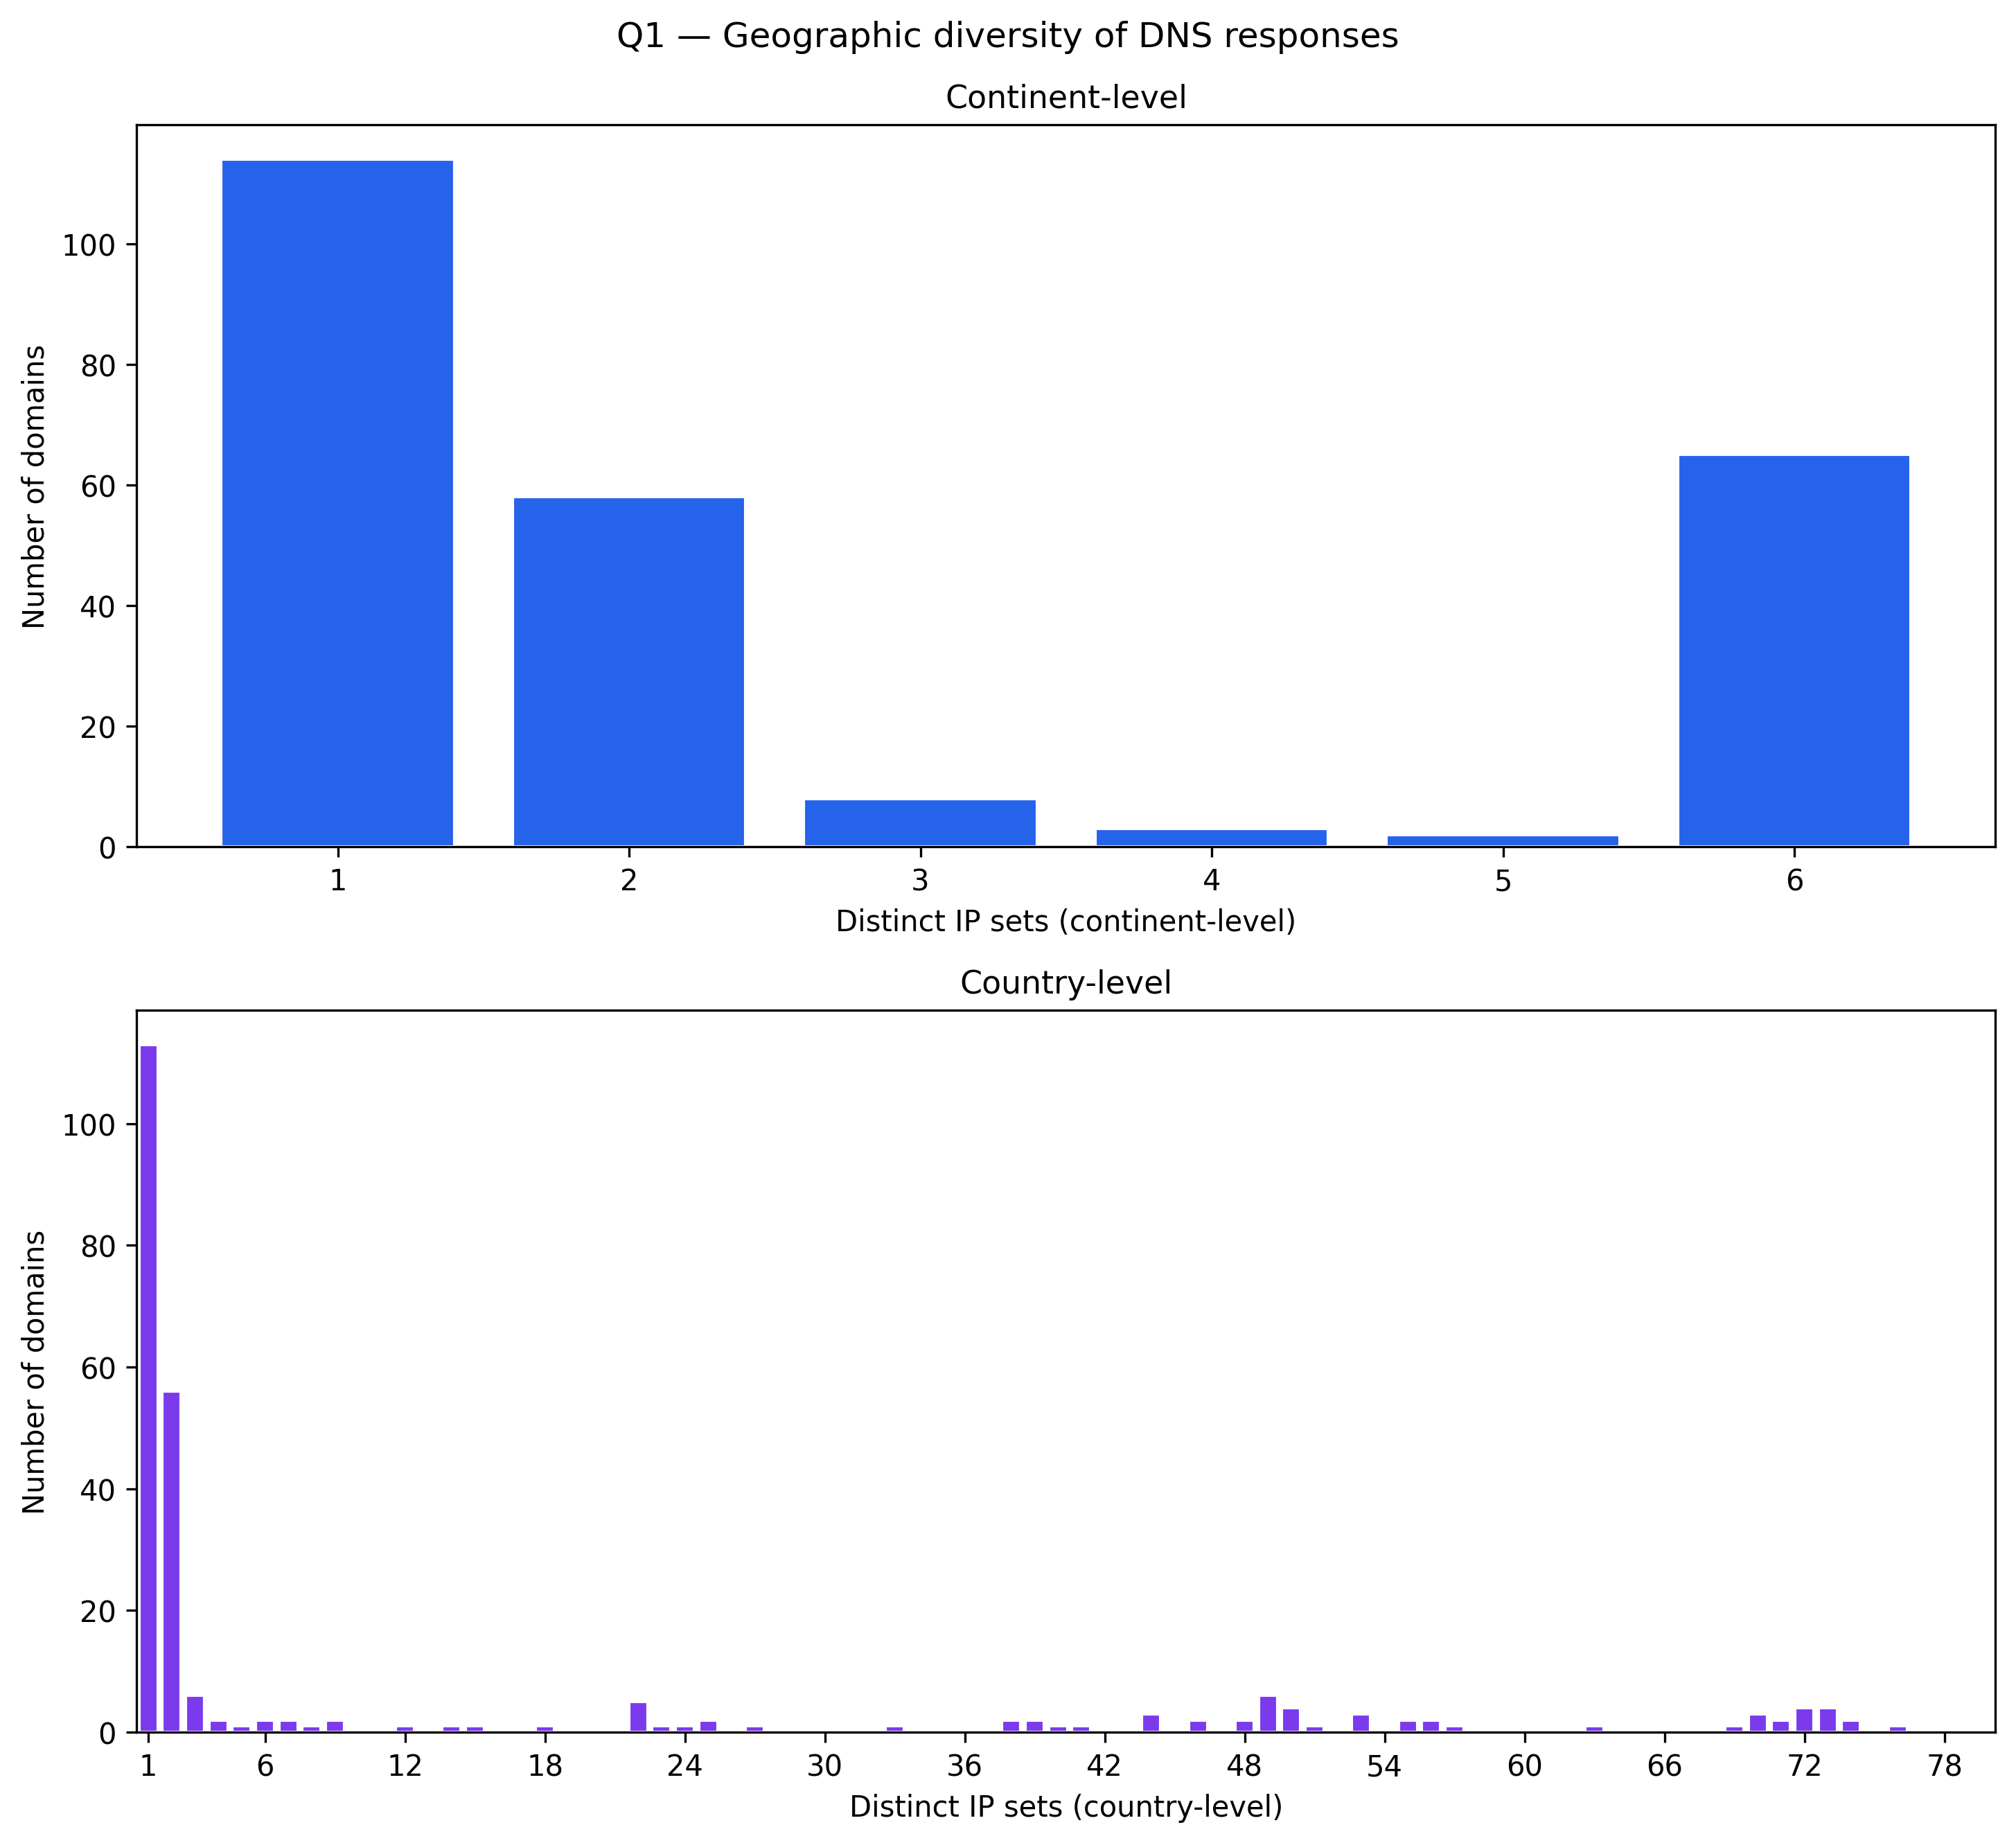
\includegraphics[width=0.85\textwidth]{figures/fig_q1a_ip_set_diversity.png}
\caption{Distribution of the number of distinct \ac{IP} address sets per domain, at two geographic granularities (50-day campaign, 45-day partial data, 247 domains). \textit{Top}: continent-level --- a value of 1 indicates a uniform response across all six continental probe groups; values above 1 indicate cross-continental differentiation. \textit{Bottom}: country-level --- the long tail reflects fine-grained \ac{CDN} routing that differentiates responses at the individual country level.}
\label{fig:q1a}
\end{figure}

\begin{figure}[H]
\centering
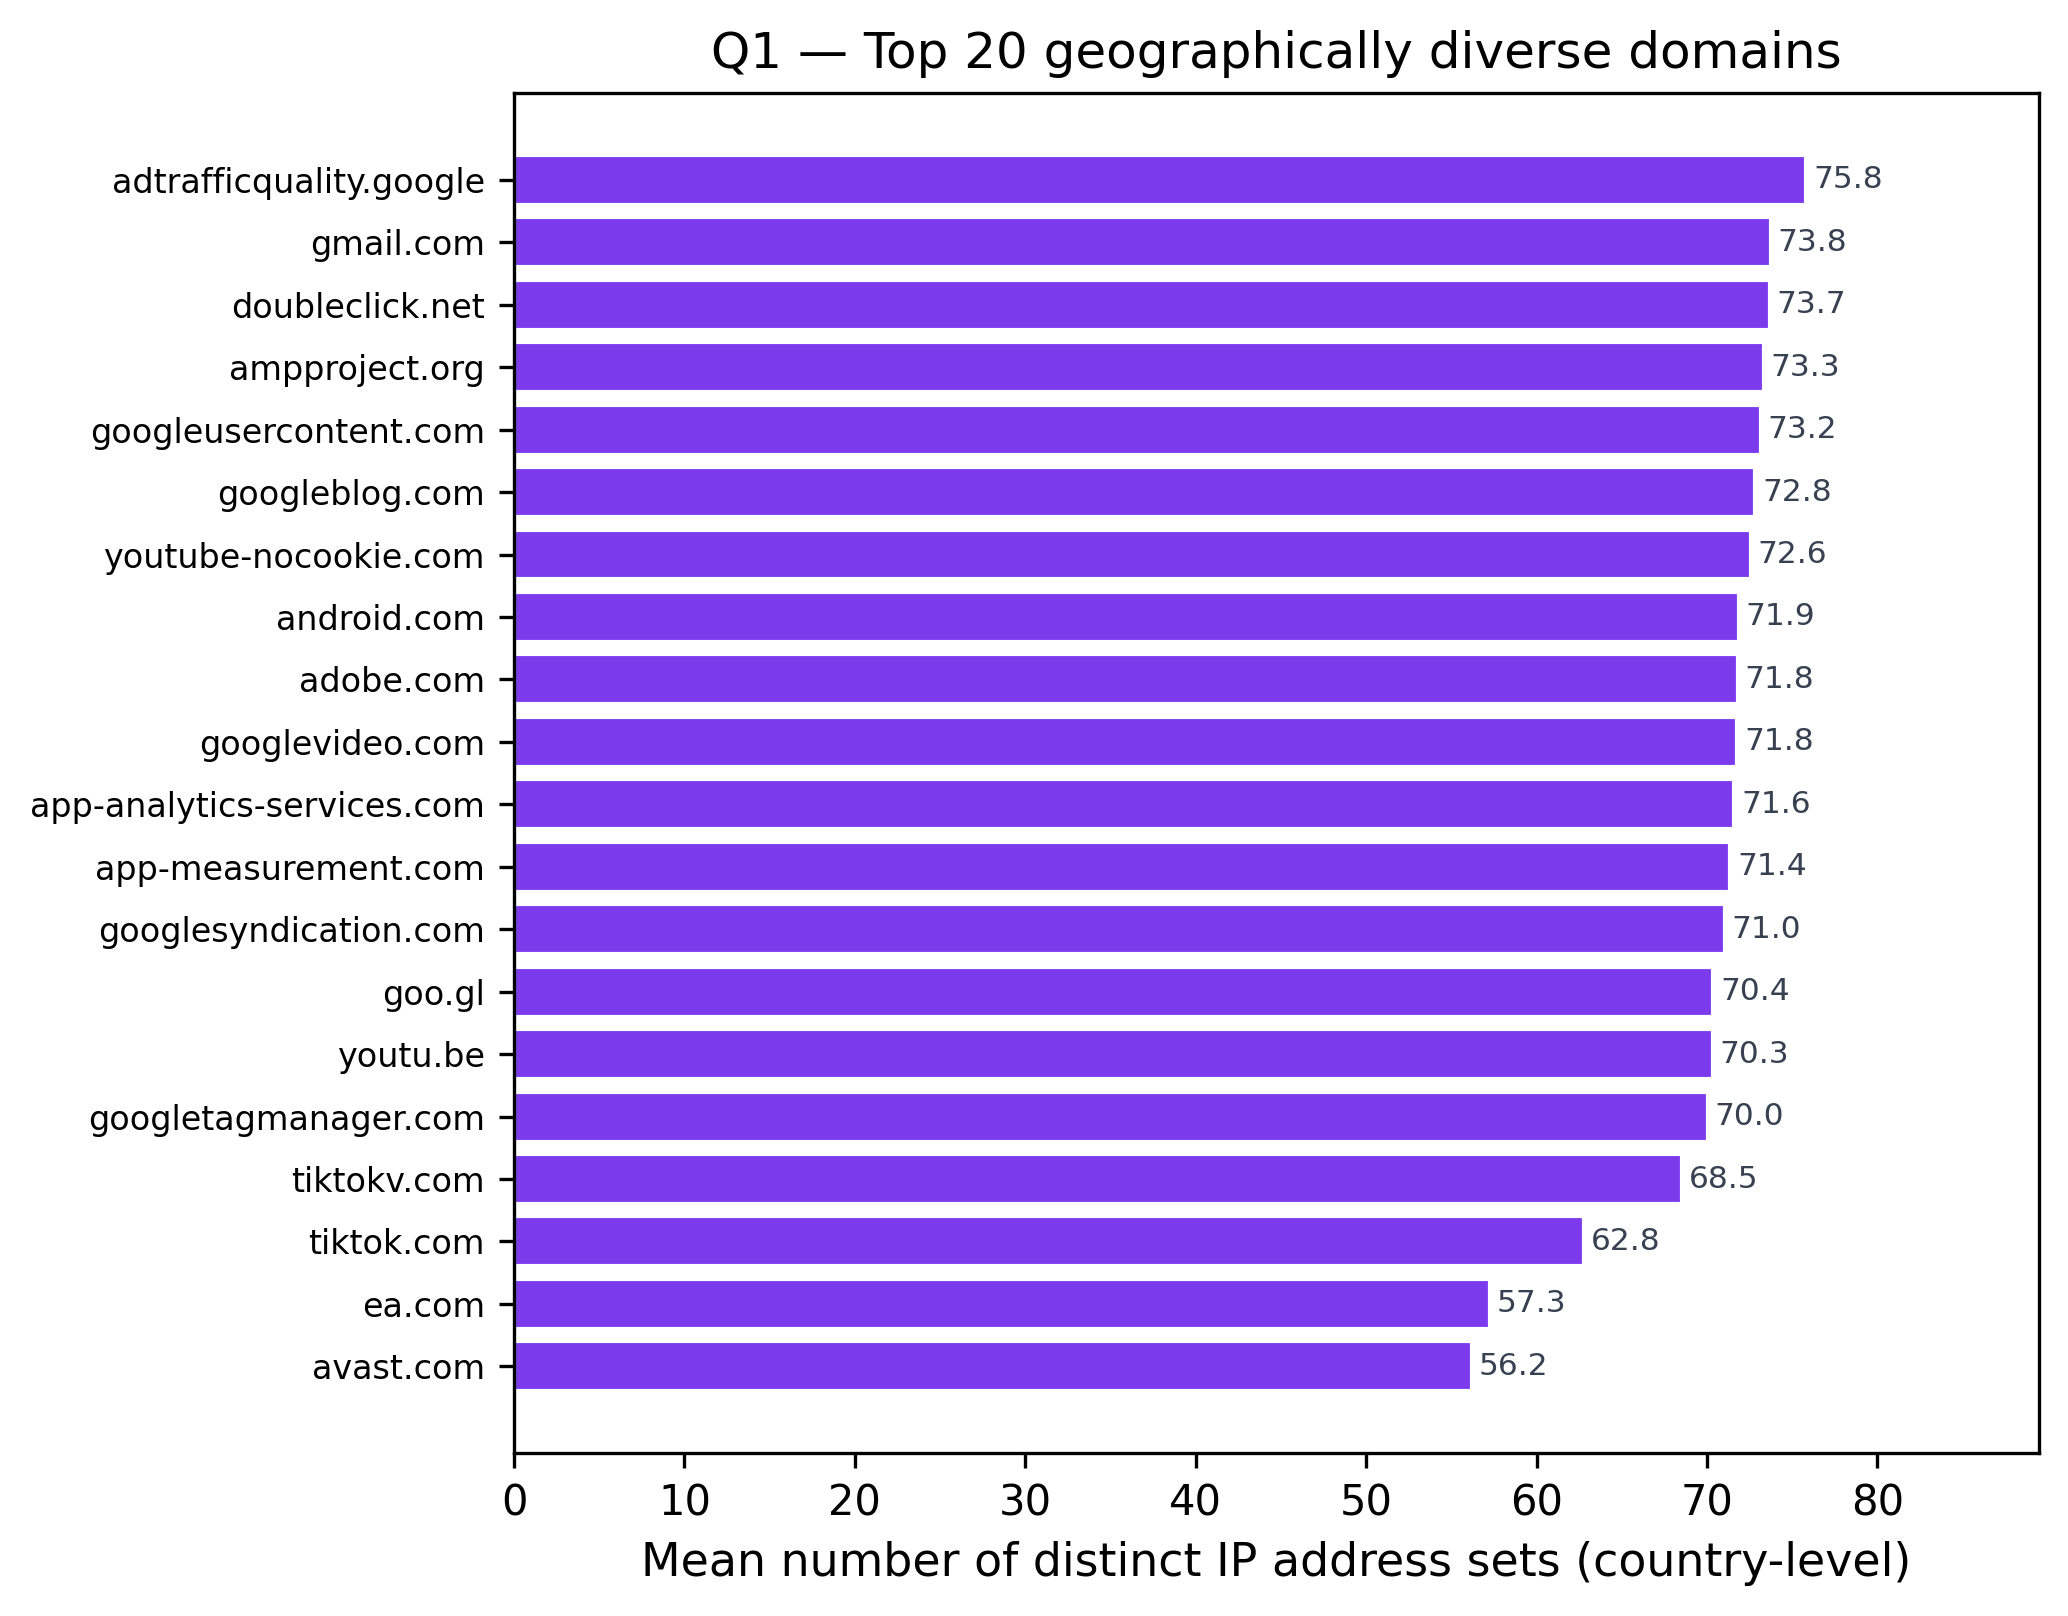
\includegraphics[width=0.85\textwidth]{figures/fig_q1b_top20_geo_diverse.png}
\caption{Top 20 most geographically diverse domains, ranked by mean number of distinct \ac{IP} address sets observed at the country level. Values annotated on each bar are the mean count over the 45-day partial dataset (50-day campaign).}
\label{fig:q1b}
\end{figure}

\subsection{NSID as an Anycast Indicator}
\label{subsec:4.2.2}

Of the 247 analysed domains, 191 (77.3\%) have at least one measurement result carrying an \ac{NSID} string in the OPT record of the \ac{DNS} response. \ac{NSID} is inserted by authoritative servers to identify the specific anycast instance that answered the query (\cite{RFC5001}); its presence is a strong indicator of anycast-based authoritative \ac{DNS} deployment. The high \ac{NSID} rate (77.3\% at the domain level; 51.9\% at the measurement-result level) confirms that anycast-based routing is the predominant infrastructure mechanism underlying geographic \ac{DNS} differentiation in the Tranco Top 250 corpus.

The \ac{NSID} presence rate differs between the two groups: 56.6\% of measurement results for continent-diverse domains carry an \ac{NSID} string, versus 47.3\% for uniform domains. This difference is consistent with the hypothesis that anycast infrastructure drives geographic \ac{DNS} response variation by directing queries to the physically nearest authoritative instance --- domains with anycast deployment both expose their instance identity via \ac{NSID} and return different \ac{IP}s to different regions.

\subsection{Interpretation}
\label{subsec:4.2.3}

The 59.9\% continent-level geographic diversity rate among the Tranco Top 250 is consistent with the \ac{CDN}-heavy composition of the top-ranked domains: major web properties served by Cloudflare, Akamai, Fastly, or Amazon CloudFront routinely return different \ac{IP} pools to different geographic regions. The jump from a mean of 2.67 distinct \ac{IP} sets at the continent level to 11.45 at the country level (Section~\ref{subsec:4.2.1}) indicates that \ac{CDN} operators do not simply route by continental region: they maintain fine-grained routing tables that differentiate responses at the individual country level or below.

The 50-day campaign (with 45 days of data currently available) provides a more reliable estimate of geographic diversity than the 9-day pilot phase alone: \ac{CDN} routing policies that change slowly (e.g., weekly pool rotations) are now well captured within the observation period. The remaining uncertainty is that domains with \ac{DNS}-level \ac{CDN} routing driven primarily by \ac{ECS} (Section~\ref{subsec:3.3.4}) may exhibit diversity patterns visible at the resolver level but not at the probe level, since RIPE Atlas probes use their local \ac{ISP} resolver which may or may not forward \ac{ECS} to authoritative servers.

\bigskip
\section{Results for Q2: Temporal Stability}
\label{sec:4.3}

\textbf{Research question}: What is the temporal stability of DNS responses for popular domains over day, week, and month timescales?

\subsection{Aggregate Change Rate}
\label{subsec:4.3.1}

For each (domain, probe) pair, the temporal change rate is defined as the fraction of consecutive daily measurement pairs for which the observed \ac{IP} address set changed. Table~\ref{tab:4.3} reports the aggregate change rate computed over three temporal windows: daily (consecutive-day pairs), weekly (pairs seven days apart), and monthly (pairs 30 days apart).

\begin{table}[H]
\centering
\small
\begin{tabular}{l r l}
\toprule
\textbf{Window} & \textbf{Change rate} & \textbf{Note} \\
\midrule
Daily   & 38.24\% & 44 consecutive-day pairs available \\
Weekly  & 38.29\% & 38 seven-day pairs available \\
Monthly & 38.30\% & 15 pairs available \\
\bottomrule
\end{tabular}
\caption{\ac{DNS} response change rates by temporal window (partial dataset: 2 April -- 16 May 2026; campaign total: 50 days, ending 21 May 2026)}
\label{tab:4.3}
\end{table}

The near-identical values across all three windows (38.24\%, 38.29\%, 38.30\%) indicate that the dominant change mechanism is the short-\ac{TTL} \ac{CDN} pool rotation that operates continuously, rather than episodic infrastructure events (server migrations, \ac{IP} address reallocations) that would produce a step change visible at longer timescales. In other words, a (domain, probe) pair that changes responses on consecutive days continues to change at approximately the same rate one week or one month later, suggesting a stable churn process rather than a convergent one.

With fifteen monthly comparison pairs now available, the monthly estimate of 38.30\% is well-established. The convergence of the daily, weekly, and monthly rates confirms that \ac{CDN} pool rotation behaves as a stationary process within the 50-day campaign window.

Of the 247 analysed domains, 51 (20.6\%) are classified as fully stable: their \ac{IP} address set does not change across any consecutive measurement pair within the 45-day partial observation window. The 38.24\% figure above is an aggregate rate computed across all (domain, probe, day) triplets; it is pulled down by the 20.6\% of fully stable domains that contribute zero-change pairs. The median per-domain change rate is 48.8\%, reflecting the typical behaviour of the non-stable majority: once a domain exhibits churn, it tends to change on roughly half of all daily measurement pairs.

\begin{figure}[H]
\centering
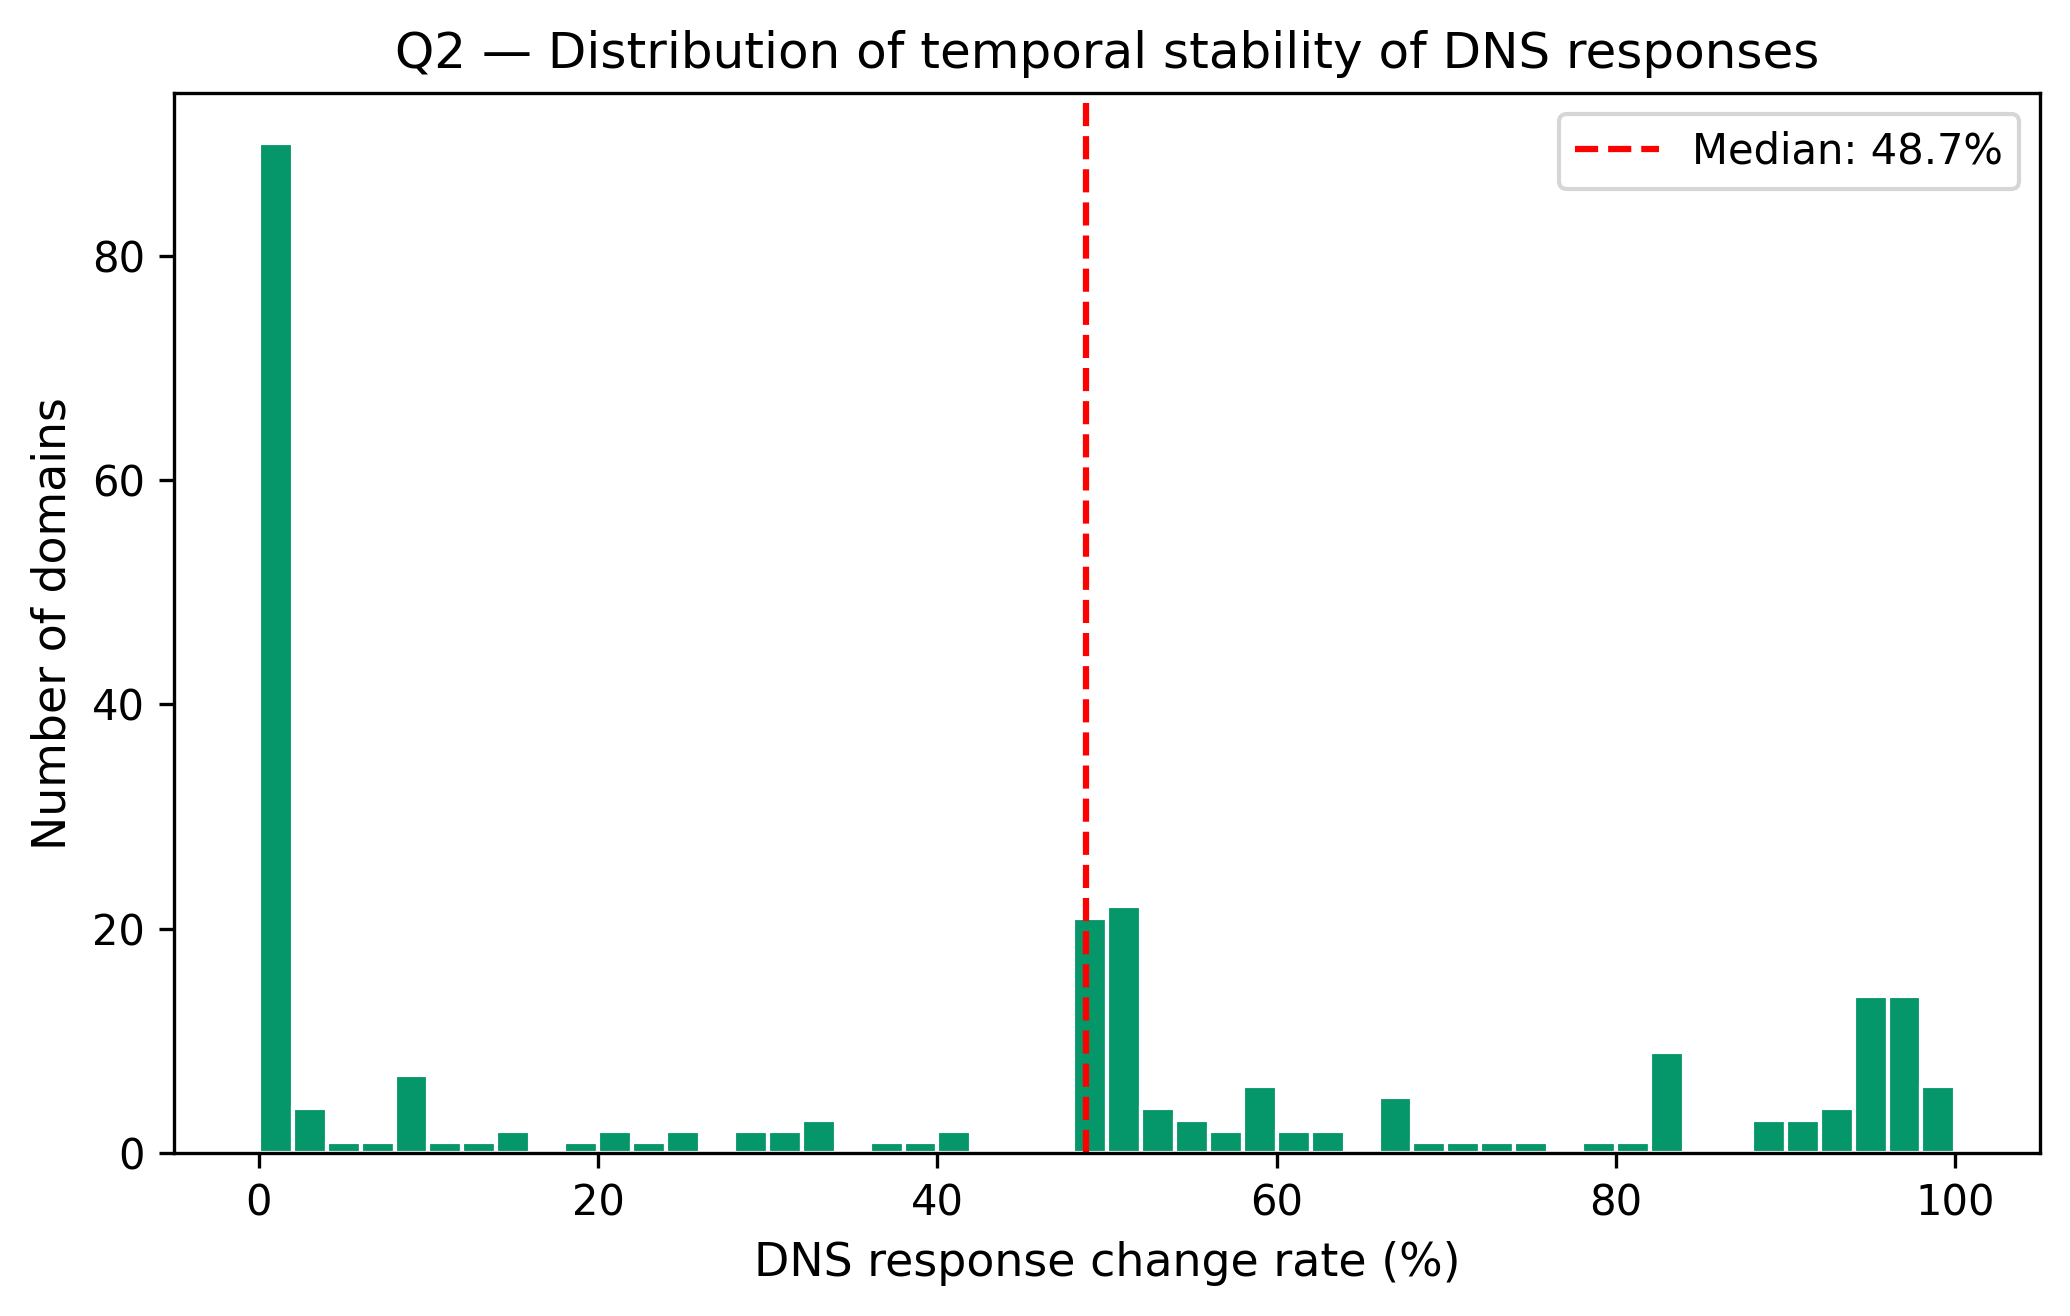
\includegraphics[width=0.85\textwidth]{figures/fig_q2_temporal_stability.png}
\caption{Distribution of per-domain \ac{DNS} response change rates over the 50-day measurement campaign (45-day partial data shown). Domains with a change rate of 0\% are fully stable (20.6\% of the corpus); the remainder show substantial daily churn, with a median of 48.8\%.}
\label{fig:q2}
\end{figure}

\subsection{Interpretation}
\label{subsec:4.3.2}

The daily change rate of 38.24\% is substantially higher than the 0.6\% daily turnover of the Tranco domain popularity ranking~\cite{LePochat2019}, confirming that \ac{DNS} response content is far more volatile than the domain popularity ordering. At approximately 64 times the list-level churn rate, this gap is expected: \ac{CDN} operators routinely configure short \ac{TTL}s (60--300 seconds for major providers) to enable rapid traffic redistribution across server pools, and RIPE Atlas probes that bypass the recursive resolver cache by querying authoritative servers directly will observe a new \ac{IP} set at each daily measurement with probability proportional to the pool rotation rate.

The bimodal character of the distribution --- approximately 20.6\% of domains are fully stable and the remainder show high churn --- corresponds to a structural split in the corpus. Fully stable domains are predominantly those with static, non-\ac{CDN} authoritative infrastructure (corporate intranets, government websites, small organisations); the high-churn majority are \ac{CDN}-backed services whose authoritative servers return dynamically load-balanced \ac{IP} pools.

The weekly rate (38.29\%) and monthly rate (38.30\%) are statistically indistinguishable from the daily rate (38.24\%), confirming that \ac{CDN} pool rotation is a stationary process across all three timescales: there is no systematic convergence or divergence within the 50-day campaign window. With fifteen monthly comparison pairs now available, this conclusion rests on solid empirical ground.

\bigskip
\section{Results for Q3: RIPE Atlas Geographic Bias Assessment}
\label{sec:4.4}

\textbf{Research question}: Do the documented geographic biases of the RIPE Atlas probe distribution significantly limit the ability to observe DNS geographic response variation?

\subsection{Bias in the Observed Probe Distribution}
\label{subsec:4.4.1}

The actual probe distribution (Table~\ref{tab:4.2}) shows that Europe and North America together account for 79.0\% of unique probe IDs, despite the geographic zone-based probe selection used for this campaign. In a perfectly balanced six-continent design each continent would hold approximately 16.7\% of probes; the actual EU+NA share of 79.0\% is nearly five times that target, confirming the well-documented structural concentration of RIPE Atlas in Western networks~\cite{Bajpai2017}.

The sampling density column (avg.\ probes/country) reveals the depth of the imbalance more starkly than raw counts alone: a European country contributes on average 142.7 probe IDs to the dataset, versus 6.2 for an African country. Asia-Pacific, despite contributing 63 countries (the most of any continent), averages only 21.3 probes per country, reflecting both the scarcity of RIPE Atlas probes in the region and the large number of countries it encompasses. Despite this concentration, the zone-based probe assignment covered 173 countries across all six continents, ensuring that global geographic coverage is maintained even if sampling density is unequal.

\subsection{Statistical Test of Measurement Impact}
\label{subsec:4.4.2}

To assess whether the geographic imbalance materially affects observed \ac{DNS} diversity, a Mann-Whitney U test compares the distribution of per-(domain, continent) unique \ac{IP} address counts between the Europe+North America group and all other continents (Asia-Pacific, Africa, South America, Oceania). The Mann-Whitney test is used because the \ac{IP}-set count distributions are heavily right-skewed and non-normal (as visible in Figure~\ref{fig:q1a}), making parametric tests inappropriate.

The test yields:
\[
U = 256{,}971.5, \quad p = 0.091
\]

The result is above the conventional $\alpha = 0.05$ threshold and is not statistically significant. Two interpretations are consistent with this finding: (1) \ac{CDN} infrastructure genuinely routes different \ac{IP} pools to different geographic regions, producing a real but modest distributional difference that the current dataset does not detect with certainty; (2) the Europe/NA-heavy probe set may undersample \ac{DNS} variation patterns specific to under-represented regions (Africa, South America, Oceania), partially masking any difference.

A second Mann-Whitney U test compares single-probe countries (34 countries with only one probe in the entire dataset) against multi-probe countries (139 countries with two or more probes), to assess whether country-level representativeness affects the diversity signal:
\[
U = 2{,}844{,}086.0, \quad p = 0.094
\]

This result also does not reach statistical significance at $\alpha = 0.05$. The direction of the effect is consistent with single-probe countries exhibiting higher variance in observed \ac{IP}-set counts (a single probe provides no within-country replication), but with the 45-day partial dataset the difference is not statistically distinguishable from sampling variability.

\begin{figure}[H]
\centering
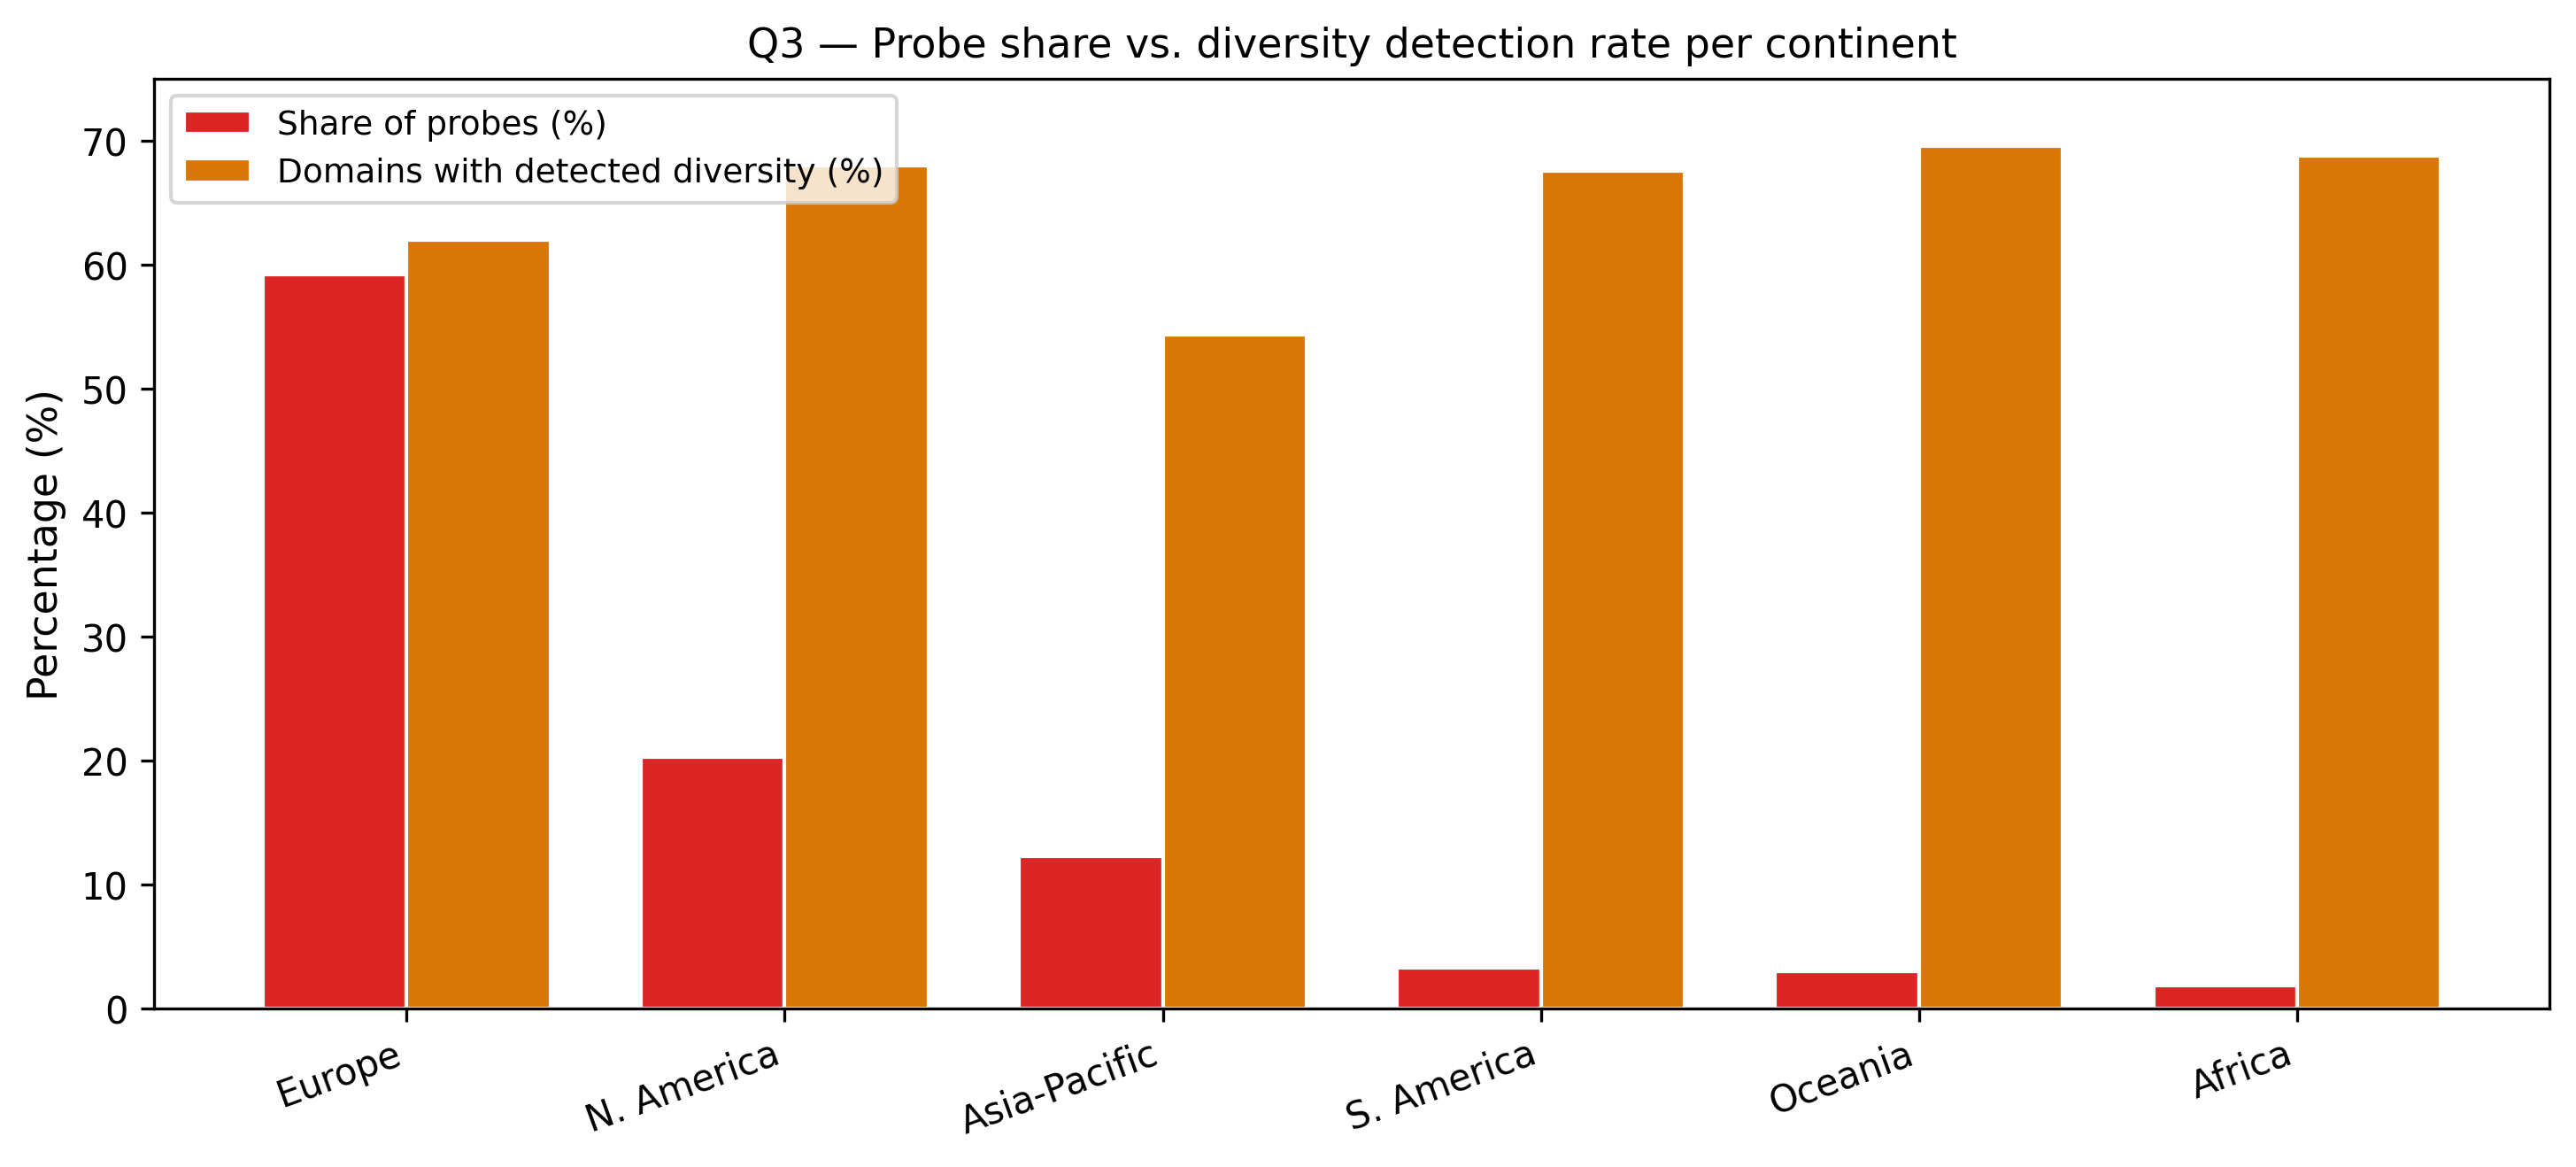
\includegraphics[width=\textwidth]{figures/fig_q3_probe_bias.png}
\caption{Probe share versus diversity detection rate per continent. Red bars show each continent's share of unique probe IDs in the dataset; orange bars show the percentage of domains for which that continent's probes detect at least one day of geographically differentiated \ac{DNS} responses. Despite holding only 2--3\% of probes, South America (58.3\%), Oceania (59.5\%), and Africa (59.5\%) detect diversity in a share comparable to or above Europe (52.6\%) and Asia-Pacific (47.4\%), which together hold 70\% of probes. This indicates that geographic probe imbalance does not prevent under-represented regions from contributing meaningful diversity observations.}
\label{fig:q3}
\end{figure}

\subsection{Interpretation}
\label{subsec:4.4.3}

Figure~\ref{fig:q3} reveals a counter-intuitive result: despite holding only 2--3\% of probes, South America (58.3\%), Oceania (59.5\%), and Africa (59.5\%) detect geographic \ac{DNS} diversity in a proportion of domains comparable to or above Europe (52.6\%) and Asia-Pacific (47.4\%), which together account for 70\% of probes. This finding suggests that probe density does not limit the ability to detect geographic diversity: even a small number of probes from an under-represented region is sufficient to observe that authoritative servers return different \ac{IP} addresses there. The Mann-Whitney test ($p = 0.091$) does not reach conventional significance, consistent with the absence of a statistically measurable difference between the EU+NA response distribution and that of other continents.

The practical implication for the 59.9\% geographic diversity rate reported in Section~\ref{sec:4.2} is nuanced: the rate is unlikely to be significantly biased downward by probe imbalance, since under-represented regions actively contribute diversity observations. The 99.6\% domain coverage per continent confirms that every region provides measurements for virtually every domain, avoiding the partial coverage problem that would make cross-continental comparisons unreliable.

\bigskip
\section{Results for Q4: Impact of Resolver Choice}
\label{sec:4.5}

\textbf{Research question}: Do the three major public \ac{DNS} resolvers (Google 8.8.8.8, Cloudflare 1.1.1.1, Quad9 9.9.9.9) return consistent \ac{DNS} responses for the same domain queried from the same geographic location, and how large is the inter-resolver divergence?

\subsection{Overview of the Q4 Campaign}
\label{subsec:4.5.1}

The Q4 campaign queried 250 domains using the same 200 RIPE Atlas probes as Q1--Q3, directing recursive \ac{DNS} queries to three public resolvers rather than to authoritative servers directly. The campaign was executed as a one-off measurement in June 2026 (measurements 177,787,616 to 179,470,557), comprising 750 individual RIPE Atlas measurements (250 domains $\times$ 3 resolvers). Each measurement targeted 200 probes, for a theoretical maximum of 50,000 probe-level results per resolver; the realised totals (Table~\ref{tab:q4_resolver_stats}) reflect a minor availability loss of 3--6\%.

\subsection{Per-Resolver Statistics}
\label{subsec:4.5.2}

\begin{table}[H]
\centering
\small
\begin{tabular}{l r r r r r}
\toprule
\textbf{Resolver} & \textbf{n (results)} & \textbf{Error rate} & \textbf{Avg RTT (ms)} & \textbf{Median RTT (ms)} & \textbf{Avg answers} \\
\midrule
Cloudflare (1.1.1.1) & 47{,}346 & 2\% & 45.8 & \textbf{15.5} & 2.27 \\
Google (8.8.8.8)     & 47{,}318 & 1\% & 50.5 & 24.7          & 2.25 \\
Quad9 (9.9.9.9)      & 47{,}067 & 1\% & 68.2 & 23.4          & 2.24 \\
\bottomrule
\end{tabular}
\caption{Q4 per-resolver statistics (250 domains, 200 probes, one-off campaign, June 2026)}
\label{tab:q4_resolver_stats}
\end{table}

Error rates are uniformly low across the three resolvers (1--2\%), confirming the availability reliability of these public services. The performance gap is more pronounced: Cloudflare's median \ac{RTT} of 15.5\,ms is 37\% lower than Google's (24.7\,ms) and 34\% lower than Quad9's (23.4\,ms). The mean \ac{RTT} values are substantially higher (45.8, 50.5, and 68.2\,ms respectively), reflecting the strongly right-skewed distribution caused by high-latency probes in Africa, Oceania, and South America. Figure~\ref{fig:q4a} illustrates both metrics.

\begin{figure}[H]
  \centering
  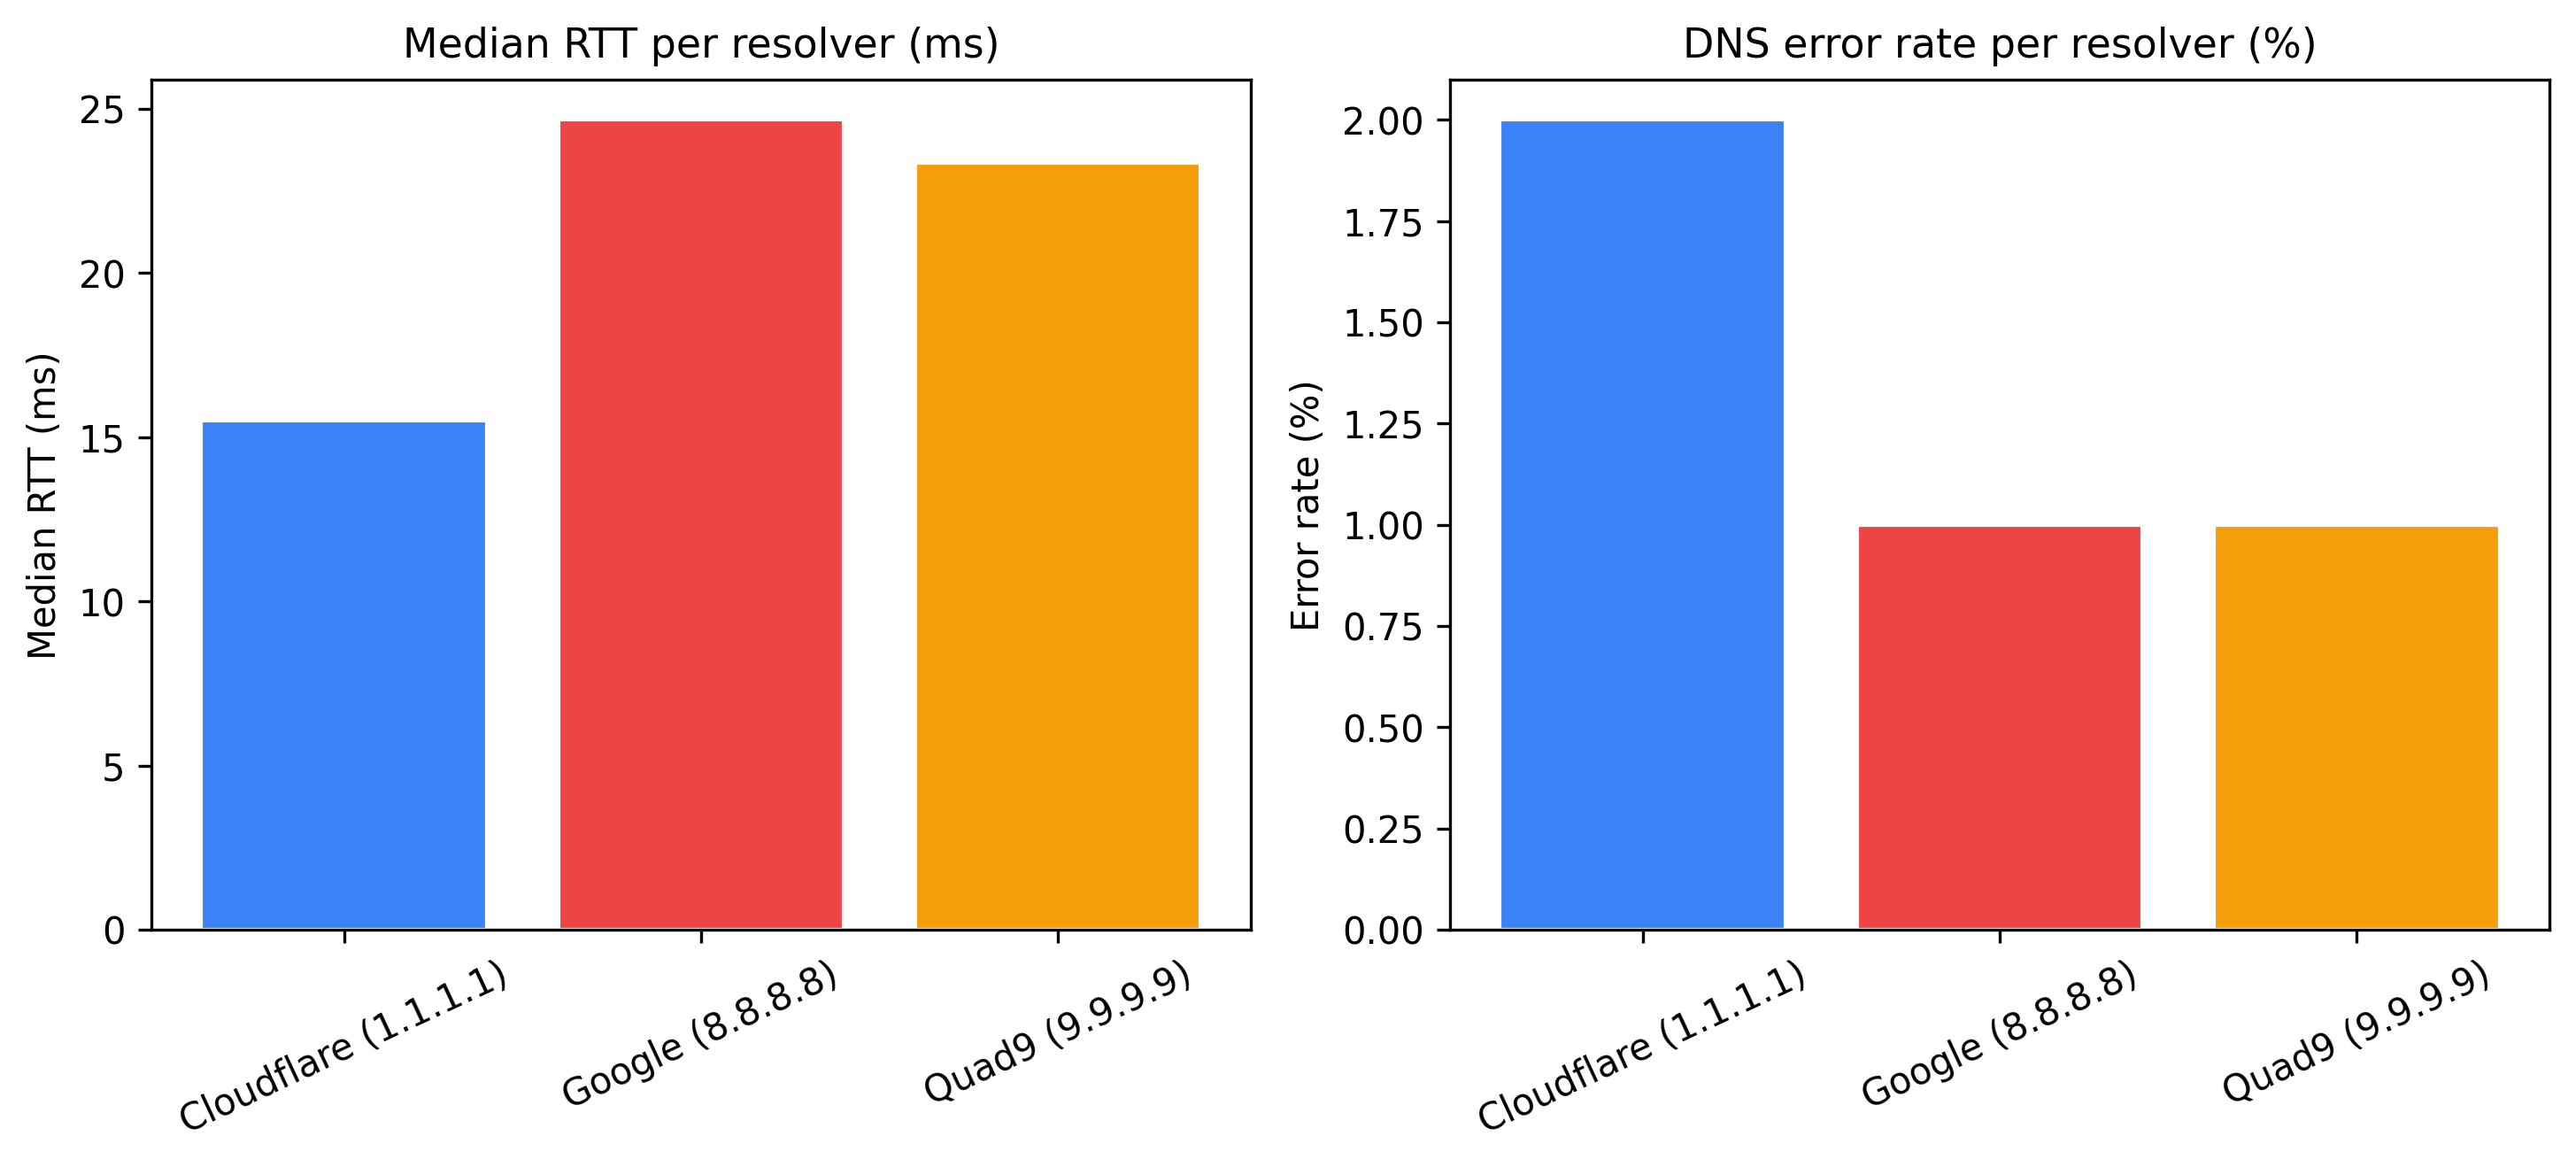
\includegraphics[width=0.92\textwidth]{figures/fig_q4_resolver_comparison.png}
  \caption{Q4 — Median RTT and error rate per public resolver (250 domains, 200 probes)}
  \label{fig:q4a}
\end{figure}

The mean answer count (2.24--2.27) is nearly identical across resolvers, indicating that all three retrieve the same number of \ac{IP} addresses for a given domain in expectation. The divergence analysis below clarifies whether those addresses are geographically equivalent.

\subsection{Cross-Resolver IP Divergence}
\label{subsec:4.5.3}

For each (domain, probe) pair with responses from all three resolvers, the returned \ac{IP} sets are compared pairwise. A divergence event is recorded when the two \ac{IP} sets are completely disjoint (no shared address). Table~\ref{tab:q4_divergence} reports the divergence rates for all three resolver pairs.

\begin{table}[H]
\centering
\small
\begin{tabular}{l r}
\toprule
\textbf{Resolver pair} & \textbf{Divergence rate (\% disjoint IP sets)} \\
\midrule
Cloudflare vs Google & 51.83\% \\
Cloudflare vs Quad9  & 52.81\% \\
Google vs Quad9      & 54.99\% \\
\bottomrule
\end{tabular}
\caption{Q4 cross-resolver \ac{IP} divergence: fraction of (domain, probe) pairs returning completely disjoint \ac{IP} sets}
\label{tab:q4_divergence}
\end{table}

More than half of all (domain, probe) observations yield entirely different \ac{IP} addresses depending on which public resolver is queried. The divergence rates are remarkably consistent across the three pairs (51--55\%), indicating that the phenomenon is not specific to any single resolver but is a structural property of the public \ac{DNS} resolution ecosystem. Figure~\ref{fig:q4b} visualises these rates.

\begin{figure}[H]
  \centering
  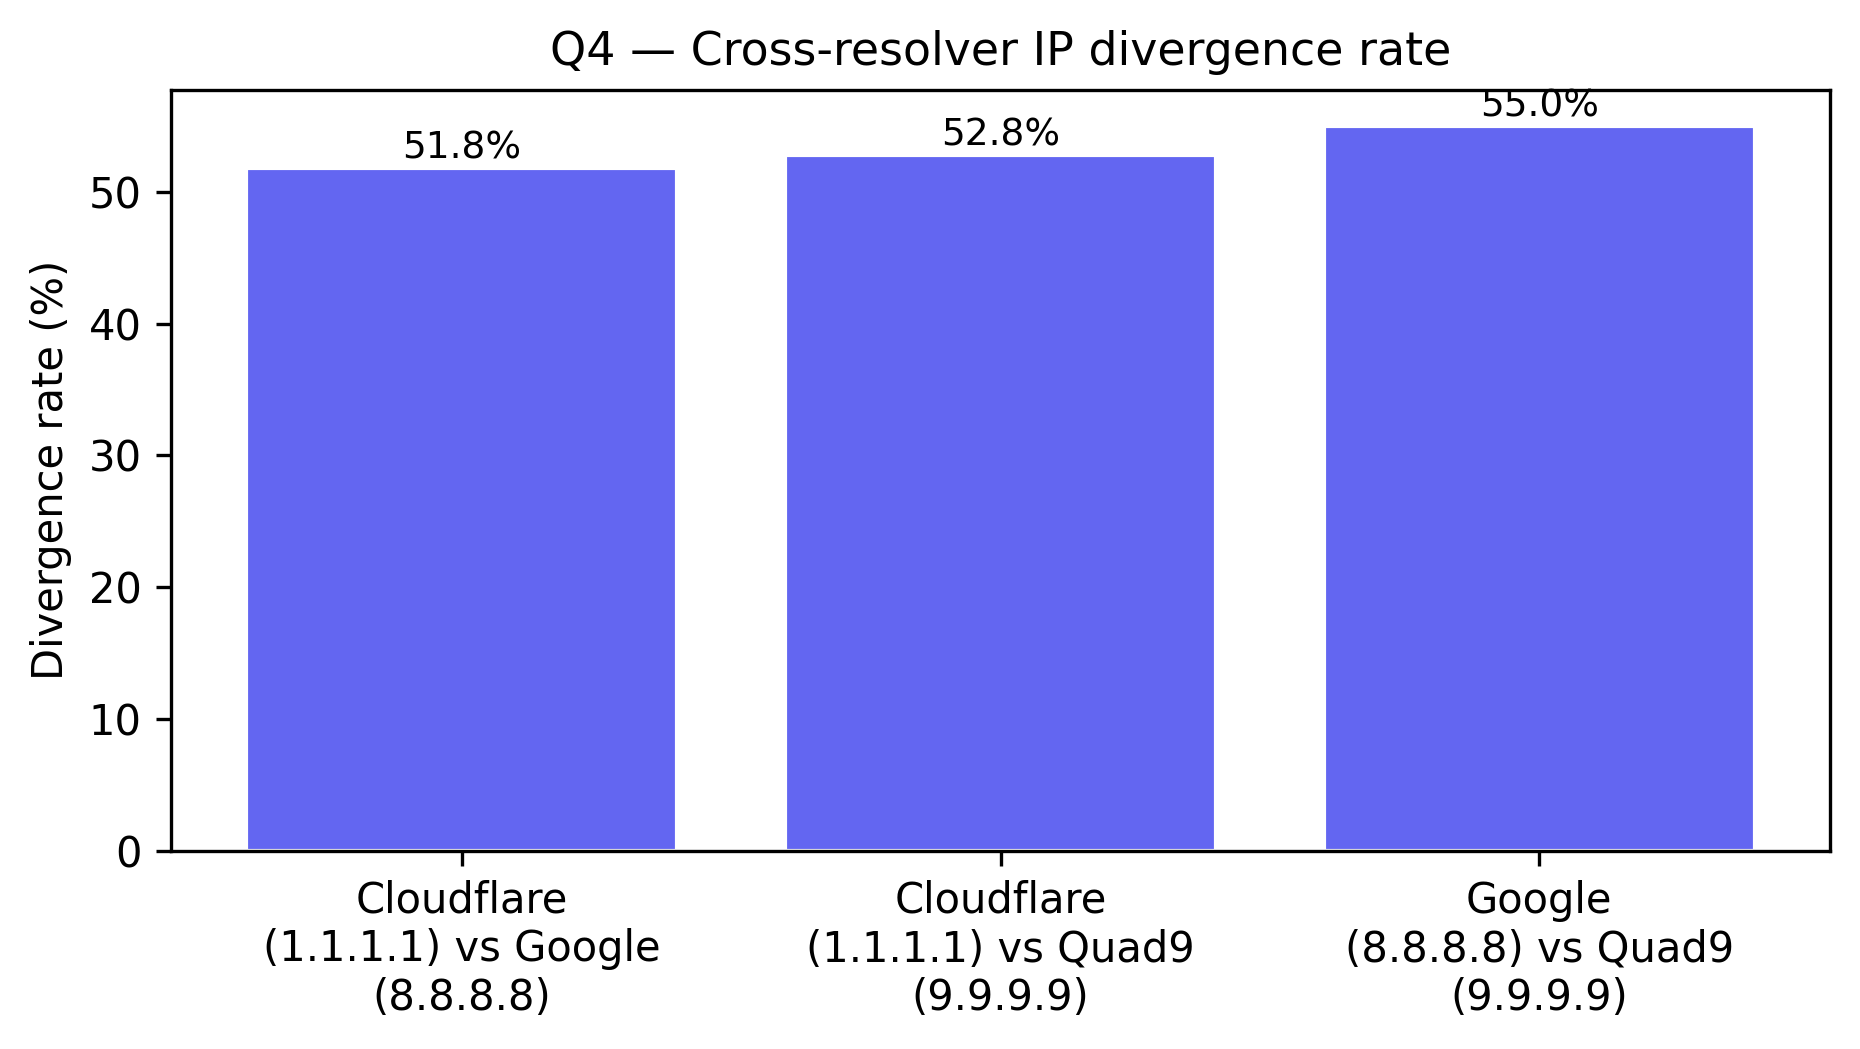
\includegraphics[width=0.72\textwidth]{figures/fig_q4b_divergence.png}
  \caption{Q4 — Cross-resolver \ac{IP} divergence rate: fraction of (domain, probe) pairs with completely disjoint \ac{IP} sets}
  \label{fig:q4b}
\end{figure}

Two mechanisms jointly explain this result. First, all three resolvers operate global anycast networks: Google 8.8.8.8, Cloudflare 1.1.1.1, and Quad9 9.9.9.9 each have hundreds of \ac{PoP}s worldwide with partially independent routing tables. A query from a given probe reaches whichever anycast instance wins the \ac{BGP} routing competition for that resolver's prefix. The winning instance forwards the query from its own \ac{IP} space, which \ac{CDN} authoritative servers use to assign a geographically optimised answer pool. Since different resolver anycast instances are co-located with different \ac{ISP}s and in different cities, the same probe may reach geographically distinct forwarding points depending on which resolver it queries, yielding different \ac{CDN}-assigned \ac{IP} pools.

Second, the three resolvers differ substantially in their \ac{EDNS} Client Subnet (\ac{ECS}) policies~\cite{RFC7871}: Cloudflare forwards the full client \ac{IP} prefix to authoritative servers by default, while Google forwards a /24 prefix, and Quad9 suppresses \ac{ECS} entirely for privacy. \ac{CDN} authoritative servers that implement \ac{ECS}-aware routing (a practice documented by Wang et al.~\cite{Wang2018} and Hours et al.~\cite{Hours2016}) therefore receive different geographic signals from the three resolvers and respond with different \ac{IP} pools for the same domain. The effect is especially pronounced for major \ac{CDN}-backed properties, which constitute the majority of the Tranco Top-250 corpus.

\bigskip
\section{Summary of Partial Results}
\label{sec:4.6}

\subsection{Answers to the Research Questions}
\label{subsec:4.6.1}

\textbf{Q1 --- Geographic diversity}: 59.9\% of Tranco Top 248 domains (148 of 247 analysed) return geographically differentiated \ac{DNS} responses at the continent level over the 50-day measurement campaign (based on 45-day partial data). At the country level, 60.3\% of domains (149 of 247) show differentiation. The mean number of distinct \ac{IP} address sets is 2.67 per domain at the continent level and 11.45 at the country level. The 77.3\% \ac{NSID} presence rate confirms that anycast-based authoritative \ac{DNS} deployment is the predominant infrastructure mechanism.

\textbf{Q2 --- Temporal stability}: The daily \ac{DNS} response change rate is 38.24\%, and the weekly (38.29\%) and monthly (38.30\%) rates are nearly identical across 44, 38, and 15 pairs respectively (45-day partial data; final dataset will yield approximately 49, 43, and 20 pairs), confirming a stationary churn process driven by \ac{CDN} pool rotation. Of 247 domains, 20.6\% are fully stable; the median per-domain change rate is 48.8\%.

\textbf{Q3 --- RIPE Atlas geographic bias}: The actual probe distribution (EU 57.8\%, NA 21.2\%, AP 12.4\%, SA 3.4\%, OC 3.2\%, AF 2.0\%) is heavily concentrated in Europe and North America (79.0\% combined). A Mann-Whitney U test yields $U = 256{,}971.5$, $p = 0.091$, above the $\alpha = 0.05$ significance threshold. Crucially, under-represented continents --- Africa (59.5\%), South America (58.3\%), and Oceania (59.5\%) --- each detect geographic diversity in more than 58\% of domains despite holding only 2--3\% of probes, at or above the Europe rate (52.6\%), indicating that the zone-based probe assignment preserves diversity observability across all regions.

\textbf{Q4 --- Resolver impact}: The three public resolvers show low and consistent error rates (1--2\%) but significantly different latency profiles: Cloudflare's median \ac{RTT} of 15.5\,ms is 37\% lower than Google (24.7\,ms) and Quad9 (23.4\,ms). More strikingly, the cross-resolver \ac{IP} divergence rate exceeds 50\% for all three resolver pairs (51.8\%–55.0\%), meaning that for more than half of (domain, probe) observations, two public resolvers return completely different \ac{IP} addresses for the same domain from the same location. This is driven by both anycast routing differences and divergent \ac{ECS} policies between resolvers.

\subsection{Result Limitations}
\label{subsec:4.6.2}

The results presented in this chapter are subject to the following constraints:

\begin{itemize}
  \item \textbf{Measurement duration}: The 50-day campaign (2 April -- 21 May 2026) will yield approximately 49 daily pairs, 43 weekly pairs, and 20 monthly comparison pairs for Q2. The 45-day partial dataset already provides reliable estimates across all three windows; the monthly estimate of 38.30\% rests on fifteen pairs and is well-established.
  \item \textbf{Phase transition}: The first nine days (pilot) used 99 domains and 50 probes; the following 41 days of the main phase (11 April -- 21 May 2026) use 248 domains and 200 probes. Analyses covering the mixed 45-day window combine these two experimental conditions; domain-level results are consistent because the main-phase corpus is a superset of the pilot corpus, but probe-count differences may affect per-domain diversity estimates.
  \item \textbf{Platform bias}: Despite geographic stratification, RIPE Atlas probe coverage remains heavily concentrated in Europe (57.8\%). The Q3 analysis shows that this imbalance does not prevent under-represented regions from detecting geographic diversity, but the lower probe density in Africa, South America, and Oceania reduces within-region statistical reliability (higher variance per single-probe country).
  \item \textbf{Domain coverage}: The analysis covers the Tranco Top 250 only. Of the 250 domains in the corpus, 2 were excluded during pre-validation because their authoritative name server \ac{IP} address could not be resolved (see Section~\ref{subsec:3.2.3}), leaving 248 active RIPE Atlas measurements. A further domain produced no valid results during the campaign and was excluded from analysis, resulting in a final corpus of 247 domains.
  \item \textbf{\ac{IPv4} only}: All measurements query \ac{DNS} \ac{A} records over \ac{IPv4}. \ac{AAAA} records and \ac{IPv6} transport are not covered. \ac{IPv6} \ac{CDN} deployment may exhibit different geographic routing patterns, and the results presented here do not characterise the \ac{IPv6} \ac{DNS} landscape.
\end{itemize}

\chapter{Discussion and Conclusion}
\label{ch:conclusion}
\iffalse
\fi
\section{Discussion of Results}
\label{sec:5.1}

The four research questions formulated in Chapter~\ref{ch:introduction} guided both the design of the measurement campaign (Chapter~\ref{ch:method}) and the presentation of empirical results (Chapter~\ref{ch:results}). This section interprets those results in light of the existing literature and draws out practical implications for measurement methodology. The campaign spans 127 measurement days (2 April -- 8 August 2026).

\bigskip
\subsection{Interpreting Geographic Diversity (Q1)}
\label{subsec:5.1.1}

\textbf{Principal finding.} Within the analysed corpus of 250 domains from the Tranco Top 250, macro-regional evaluation reveals that 69.6\% exhibit geographic diversity at the continental scale, resolving to distinct \ac{IP} address pools for probes across at least two continents on one or more measurement days. The rate is identical at national resolution (69.6\%), while 69.2\% of domains also exhibit detectable intra-continental differentiation within the same regional block. Across the 185 countries monitored, domains yield a mean of 13.7 unique \ac{IP} sets, underscoring the fine-grained nature of \ac{CDN} traffic engineering operating well below continental boundaries.

\textbf{Comparison with the literature.}

Van Rijswijk-Deij~\cite{vanRijswijk2016} highlighted that OpenINTEL, operating from a single vantage point in the Netherlands, is structurally blind to any geographic differentiation that authoritative servers implement via anycast or \ac{ECS}. Our distributed architecture --- measurements across 185 countries --- directly addresses this gap. The 69.6\% continent-level diversity rate empirically quantifies the fraction of popular domains whose \ac{DNS} responses OpenINTEL cannot fully characterise: a single-location observatory would observe uniform responses for nearly one third of the Tranco Top-250.

Koch~\cite{Koch2021} showed that the application context determines whether anycast routing introduces operationally significant response variation. The 88.8\% domain-level \ac{NSID} presence rate confirms that anycast-based authoritative \ac{DNS} is the primary structural mechanism underlying geographic response differentiation, consistent with Koch's conclusion.

The mean of 13.7 distinct \ac{IP} address sets at the country level versus 2.65 at the continent level indicates that \ac{CDN} routing granularity is substantially finer than continental boundaries, consistent with Li~\cite{Li2025} and Hours~\cite{Hours2016}: major \ac{CDN} operators maintain country-level routing tables that produce distinct \ac{IP} pools even within the same continent.

\textbf{Inter-campaign finding.} Breaking the analysis by campaign, 60.3\% of common domains are classified as continent-diverse in Campaign~1 (zone-based selection) against 49.7\% in Campaign~2 (continent-stratified fixed set). The lower Campaign~2 rate --- despite broader geographic coverage across Asia-Pacific and Africa --- reflects the reduced EU and NA probe density: fine-grained Western \ac{CDN} routing differences account for a significant share of detectable continent-level diversity, and Campaign~2's 14 European probes are insufficient to capture them. The combined 69.6\% rate benefits from pooling both campaigns over 127 days.

\textbf{Practical implications.}
\begin{itemize}
  \item \textit{For longitudinal \ac{DNS} observatories:} Any measurement system that aims to characterise the \ac{DNS} responses returned to end users in different geographic regions must operate from multiple vantage points. Even a small number of geographically distributed probes suffices to detect geographic variation invisible to single-site measurement.
  \item \textit{For probe selection strategy:} Zone-based selection maximises diversity detection probability in Western \ac{CDN}-heavy corpora; continent-stratified selection reveals richer per-region characterisation at the cost of lower aggregate detection rates. Neither strategy dominates: the optimal design combines a minimum Western probe quota with broad geographic coverage.
  \item \textit{For network performance researchers:} Studies using \ac{DNS} records to infer content-server location should account for geographic diversity; for 69.6\% of popular domains, the \ac{IP} address seen from one location does not represent the \ac{IP} address seen from another.
\end{itemize}

\bigskip
\subsection{Interpreting Temporal Stability (Q2)}
\label{subsec:5.1.2}

\textbf{Principal finding.} The aggregate daily \ac{DNS} response change rate is 38.09\%, and the median per-domain change rate is 48.76\%. Of 250 domains, 17.6\% are fully stable; the remainder exhibit substantial daily churn. The weekly (38.17\%) and monthly (38.18\%) rates are statistically indistinguishable from the daily rate across approximately 97 monthly comparison windows, suggesting that \ac{CDN} pool rotation is a stationary process across all three timescales over four months of continuous measurement.

\textbf{Comparison with the literature.}

Le Pochat~\cite{LePochat2019} measured a 0.6\% daily change rate in the Tranco list composition itself. Our per-domain \ac{DNS} change rates of 38.09\% are therefore approximately 63 times higher than the list-level churn, confirming that a stable corpus of popular domains does not imply stable \ac{DNS} records. The \ac{DNS} layer is substantially more volatile than the popularity-ranking layer, consistent with the short \ac{TTL}s (60--300 seconds) that major \ac{CDN} operators configure to enable rapid traffic redistribution.

Van Rijswijk-Deij~\cite{vanRijswijk2016} demonstrated that \ac{DNS} infrastructure evolves on timescales ranging from hours (\ac{TTL}-driven updates) to years (infrastructure migrations). Our 127-day campaign captures the short-to-medium end of this spectrum. The near-identity of daily, weekly, and monthly change rates (38.09\%, 38.17\%, 38.18\%) confirms that the dominant mechanism is high-frequency \ac{CDN} pool rotation rather than episodic infrastructure events. With approximately 97 monthly comparison windows available, this conclusion rests on substantially stronger empirical ground than a 50-day campaign would provide.

\textbf{Practical implications.}
\begin{itemize}
  \item \textit{Optimal measurement frequency:} For the 17.6\% of fully stable domains, weekly snapshots suffice. For the high-churn majority (median 48.76\%), daily measurement is necessary.
  \item \textit{\ac{DNS} archival strategy:} A tiered policy --- daily collection for volatile domains, weekly for stable ones --- would reduce measurement volume while preserving near-complete change coverage.
\end{itemize}

\bigskip
\subsection{Interpreting the Impact of Geographic Bias (Q3)}
\label{subsec:5.1.3}

\textbf{Principal finding.} Campaign~1's zone-based probe selection concentrates 79.5\% of probe IDs in Europe and North America, consistent with the structural composition of the RIPE Atlas platform; Campaign~2's continent-stratified set reduces this to 20.6\%. Across both campaigns, the Mann-Whitney U test comparing EU+NA against all other continents yields $p = 0.292$, above the $\alpha = 0.05$ threshold: the continental-level imbalance does not statistically distort diversity detection. However, the comparison of 35 single-probe countries against 150 multi-probe countries yields $p \approx 10^{-13}$: countries covered by only one probe observe significantly fewer unique \ac{IP} sets, indicating that within-country probe density matters for the richness of diversity characterisation.

\textbf{Comparison with the literature.}

Bajpai~\cite{Bajpai2017} quantified the RIPE Atlas probe distribution and noted that 91\% of active nodes were confined to Europe and North America. Campaign~1's zone-based selection reproduces this skew (79.5\% EU+NA), confirming that zone rotation alone cannot overcome the structural deficit. Campaign~2 demonstrates that explicit continent-stratified allocation substantially corrects this bias, though the absolute scarcity of RIPE Atlas infrastructure in Africa --- yielding only 39 probes across 34 nations in Campaign~2 --- presents a physical deployment ceiling that algorithmic selection cannot fully overcome.

\textbf{Counter-intuitive finding.} Despite holding only 2.2\% of probe IDs in Campaign~1, Africa detects geographic \ac{DNS} diversity in a share of domains comparable to Europe. This is rooted in \ac{CDN} traffic engineering: operators allocate distinct \ac{IP} pools specifically tailored to Africa, so even a single African probe reliably returns an \ac{IP} footprint segregated from the European pool. The EU+NA imbalance does not create a detection blind spot, but the significant single vs.\ multi-probe result establishes that it does limit the \emph{depth} of characterisation: adding more probes per country reveals additional routing granularity invisible to single-probe coverage.

\textbf{Practical implications.}
\begin{itemize}
  \item \textit{For Q1 robustness:} The 69.6\% geographic diversity rate is robust to the continental probe imbalance (EU+NA $p = 0.292$), since under-represented regions detect comparable per-domain diversity to Europe.
  \item \textit{On the value of stratified allocation:} Campaign~2 demonstrates that explicit continent-stratified allocation substantially corrects the Western probe bias and reveals richer per-region \ac{IP} diversity (e.g., 9.4 vs 5.3 mean unique \ac{IP} sets per domain in Africa). However, the reduction in EU and NA probe density suppresses aggregate diversity detection by approximately 10 percentage points on the common domain corpus. A hybrid design --- continental stratification with a guaranteed minimum EU/NA quota --- would mitigate this trade-off.
  \item \textit{For probe deployment priorities:} Future campaigns should prioritise increasing \emph{per-country} probe density (not just country breadth) in Africa and Asia-Pacific, to transition from binary diversity detection toward statistically robust intra-regional routing characterisation.
\end{itemize}

\bigskip
\subsection{Interpreting Resolver Impact (Q4)}
\label{subsec:5.1.4}

\textbf{Principal finding.} For 52--55\% of (domain, probe) pairs, the three major public resolvers return different \ac{IP} address sets for the same domain queried from the same geographic vantage point. Divergence rates are consistent across all resolver pairs (CF/G: 51.83\%, CF/Q9: 52.81\%, G/Q9: 54.99\%). Cloudflare achieves the lowest median latency (15.5~ms), substantially below Google (24.7~ms) and Quad9 (23.4~ms), reflecting its denser anycast deployment.

\textbf{Comparison with the literature.}

Hours~\cite{Hours2016} demonstrated that clients routed through Google \ac{DNS} were directed to Akamai servers 20~ms farther in \ac{RTT} terms, confirming that resolver choice affects \ac{CDN} edge assignment. Our result extends this finding to a corpus-scale measurement: for more than half of all (domain, probe) pairs across 250 popular domains, the choice between Cloudflare, Google, and Quad9 determines a different \ac{IP} address outcome. This is not a marginal effect confined to specific \ac{CDN} providers --- it is a systematic, corpus-wide property of the resolver ecosystem.

Wang~\cite{Wang2018} documented that routing mismatches caused by resolver centralization can inflate server distance by up to 113\%. Our result provides a measurement-based lower bound: 52--55\% of queries receive a resolver-specific \ac{IP} that differs from at least one other major resolver's answer, implying that the choice of resolver is a first-order determinant of \ac{CDN} edge assignment, comparable in magnitude to the effect of the probe's geographic location established in Q1.

\textbf{Practical implications.}
\begin{itemize}
  \item \textit{For end-user performance:} Users who switch between public resolvers can expect different \ac{CDN} edge assignments for a majority of popular domains, with potential \ac{RTT} and throughput consequences.
  \item \textit{For \ac{DNS} measurement methodology:} Studies that use \ac{DNS} records to infer \ac{CDN} topology or content-server geography must specify which resolver was used; results from Cloudflare, Google, and Quad9 are not interchangeable for more than half of popular domains.
\end{itemize}

\bigskip
\section{Limitations of the Study}
\label{sec:5.2}

\bigskip
\subsection{Methodological Limitations}
\label{subsec:5.2.1}

\textbf{Collection period.} Spanning 127 days (2 April -- 8 August 2026), this campaign captures short-to-medium-term operational dynamics. Broader cyclical or seasonal trends --- strategic \ac{CDN} capacity expansions ahead of peak traffic periods, long-term infrastructural migrations, or the routing impact of geopolitical events --- remain outside the scope of this temporal envelope. Van Rijswijk-Deij~\cite{vanRijswijk2016} demonstrated that multi-year longitudinal observation is necessary to characterise infrastructure evolution at scale; the current results should be understood as a temporally bounded snapshot of an inherently dynamic system.

\textbf{Domain corpus.} Focusing on the Tranco Top-250 limits the scope to the apex of global web popularity. The vast long tail of the \ac{DNS} namespace --- roughly 360 million registered domains~\cite{vanRijswijk2016} --- likely follows entirely different geographic distribution profiles and stability trends. The routing insights documented here reflect the high-traffic domain tier exclusively and cannot be extrapolated to the broader namespace.

\textbf{Geographic probe bias.} While Section~\ref{sec:4.4} establishes that the EU+NA continental imbalance does not prevent diversity detection, the significant single vs.\ multi-probe result confirms that the absolute volume of probes in Africa, South America, and Oceania constrains intra-regional statistical power.

\bigskip
\subsection{Technical Limitations}
\label{subsec:5.2.2}

\textbf{RIPE Atlas platform constraints.} The RIPE Atlas concurrent measurement limit for one-off measurements is a hard practical constraint that must be factored into study design. This limit prevented running Q4 while the 248 ongoing periodic measurements were active, requiring the Q4 campaign to be timed around campaign transitions.

\textbf{\ac{ISP} resolver not available for Q4.} The local \ac{ISP} resolver comparison planned for Q4 could not be executed: the RIPE Atlas \ac{API} rejects the combination of an explicit target \ac{IP} and \texttt{use\_probe\_resolver: true}, and probe inspection showed that a large fraction of probes forward queries to public resolvers anyway, making the condition structurally unimplementable. The Q4 results therefore characterise divergence among the three major public resolvers only, and cannot address whether \ac{ISP} resolvers would produce responses closer to the authoritative signal.

\textbf{Two-campaign heterogeneity.} The two main campaigns used different probe selection strategies (zone-based vs continent-stratified), different probe counts (200 vs 150), and partially different domain corpora (248 vs 201 active domains). Combining them in full-period analyses introduces mixed observational conditions. While the controlled inter-campaign comparison in Section~\ref{subsec:4.1.4} uses the 200 common domains to isolate the strategy effect, full-period results (69.6\% Q1 rate, 38.09\% Q2 rate) pool both conditions and should be interpreted accordingly. Separately, the 9-day pilot phase uses different probe counts and a smaller corpus, reducing its statistical weight in longitudinal analyses.

\bigskip
\subsection{Interpretive Limitations}
\label{subsec:5.2.3}

\textbf{Mechanism attribution.} The \ac{NSID} presence rate difference between diverse and uniform domains is consistent with anycast being the dominant mechanism, but does not allow us to disentangle anycast-based routing from \ac{DNS}-level \ac{CDN} routing (GeoDNS) or \ac{ECS}-driven differentiation, since all three mechanisms can produce different \ac{IP} addresses in different regions.

\textbf{Generalisation beyond the Top-250.} Because the Tranco Top-250 is heavily dominated by enterprise-grade, hyperscale \ac{CDN} deployments, the 69.6\% continent-level diversity rate represents an operational ceiling likely to overestimate the diversity profile of a broader domain sample.

\textbf{Stationarity assumption.} Our conclusion regarding the stationarity of \ac{CDN} pool rotation is supported by approximately 97 monthly comparison windows. While this provides strong evidence for short-to-medium-term stationarity, capturing potential macro-cyclical trends would require extending measurement beyond the current 127-day window.

\bigskip
\section{Contributions of This Work}
\label{sec:5.3}

\subsection{Scientific Contributions}
\label{subsec:5.3.1}

\textbf{Primary empirical contribution.}
This thesis provides a systematic, multi-vantage-point quantification of \ac{DNS} response diversity for the Tranco Top-250, based on 4,146,242 \ac{DNS} measurements from 13,083 unique RIPE Atlas probes across 185 countries over 127 measurement days. The results characterise four dimensions of \ac{DNS} behaviour at a scale and geographic resolution not previously reported for this domain corpus: geographic diversity (Q1), temporal stability (Q2), probe-bias sensitivity (Q3), and resolver-induced divergence (Q4).

\textbf{Empirical validation of literature hypotheses.} Table~\ref{tab:hypothesis_validation} summarises the validation status of key claims from the literature.

\begin{table}[H]
\centering
\small
\begin{tabularx}{\linewidth}{X p{4.0cm} p{5.5cm}}
\toprule
\textbf{Claim} & \textbf{Source} & \textbf{Status} \\
\midrule
Single-vantage-point \ac{DNS} measurement misses geographic variation & ~\cite{vanRijswijk2016} & \textbf{Confirmed}: 69.6\% of domains are continent-diverse \\
Anycast is the primary mechanism of geographic \ac{DNS} variation & ~\cite{Koch2021}; ~\cite{Bortzmeyer2013} & \textbf{Confirmed}: 88.8\% domain-level \ac{NSID} rate \\
\ac{CDN} routing operates at sub-continental granularity & ~\cite{Hours2016}; ~\cite{Li2025} & \textbf{Confirmed}: 13.7 country-level vs 2.65 continent-level \ac{IP} sets \\
\ac{DNS} response content is more volatile than domain popularity rankings & ~\cite{LePochat2019} & \textbf{Confirmed}: 38.09\% daily change rate vs 0.6\% Tranco churn \\
RIPE Atlas geographic bias persists and affects \ac{DNS} measurements & ~\cite{Bajpai2017}; ~\cite{Nosyk2025} & \textbf{Confirmed} (C1: EU+NA 79.5\%; $p=0.292$); single-probe countries observe significantly less diversity ($p \approx 10^{-13}$) \\
Resolver choice affects observed \ac{CDN} edge assignment & ~\cite{Hours2016}; ~\cite{Wang2018} & \textbf{Confirmed}: 52--55\% divergence across all resolver pairs \\
\bottomrule
\end{tabularx}
\caption{Empirical validation status of key claims from the literature}
\label{tab:hypothesis_validation}
\end{table}

\bigskip
\subsection{Methodological Contributions}
\label{subsec:5.3.2}

\textbf{Reproducible measurement pipeline.} The complete pipeline --- from probe selection and RIPE Atlas campaign configuration through data collection, Parquet storage, and statistical analysis --- is documented in Chapter~\ref{ch:method} and published as open-source code on GitHub (\url{https://github.com/ogautier-unam/dns-pipeline}). Key artefacts include the probe selection script with three-round geographic stratification, the daily fetch and parsing pipeline, and the Q1--Q4 analysis scripts.

\textbf{Two-level geographic analysis.} Our two-level analysis (continent + country) yields identical detection rates at both granularities (69.6\% at the continental and national level alike), while \ac{CDN} routing granularity is substantially finer at the country level (mean 13.7 distinct \ac{IP} sets) than at the continent level (mean 2.65 \ac{IP} sets). The separate intra-continental metric (69.2\%) confirms that virtually all continent-diverse domains also exhibit within-continent differentiation. This two-level methodology is reusable for any future distributed \ac{DNS} measurement study.

\textbf{Two-campaign comparative design.} By running consecutive campaigns with zone-based and continent-stratified probe selection, we generate empirical evidence of how probe selection strategy shapes geographic diversity detection. The comparison (Section~\ref{subsec:4.1.4}) shows that zone-based selection detects more aggregate continent-level diversity (60.3\% vs 49.7\% on common domains) while stratified selection reveals richer per-region characterisation. This controlled within-study comparison is a reusable methodological template for future probe selection experiments.

\textbf{RIPE Atlas best practices for \ac{DNS} studies.} We operationalize and build upon the campaign design principles pioneered by Bajpai~\cite{Bajpai2017}, Nosyk~\cite{Nosyk2025}, and Boswell and Perkins~\cite{Boswell2024}: geographic stratification via system tags, direct authoritative-server queries to decouple routing observations from caching artifacts, structured credit budget planning, and \ac{NSID}-based anycast instance identification.

\bigskip
\subsection{Data Contribution}
\label{subsec:5.3.3}

\textbf{Full dataset.} The 127-day measurement campaign (2 April -- 8 August 2026) generated 4,146,242 \ac{DNS} measurement results from 13,083 unique RIPE Atlas probes across 185 countries (Q1--Q3 authoritative measurements). The complete dataset in Parquet format is deposited on Zenodo~\cite{Zenodo} under CC~BY~4.0, making it permanently citable and independently verifiable in accordance with \ac{FAIR} data principles. The pipeline source code is published on GitHub under the MIT licence.

\bigskip
\section{Future Work}
\label{sec:5.4}

\bigskip
\subsection{Immediate Extensions}
\label{subsec:5.4.1}

\textbf{\ac{ISP} resolver comparison for Q4.} The most significant gap left by this study is the absence of a local \ac{ISP} resolver condition in Q4. A dedicated measurement run using \texttt{use\_probe\_resolver: true} --- without a target \ac{IP} field --- would allow comparison of \ac{ISP} resolver responses against the public resolver baselines established here. Prior filtering of probes whose \texttt{/etc/resolv.conf} points to public resolvers (rather than genuine \ac{ISP} infrastructure) would be required to ensure the condition is structurally meaningful.

\textbf{Temporal extension.} Despite covering 127 days, the campaign does not reach the multi-year timescales that Van Rijswijk-Deij~\cite{vanRijswijk2016} identified as necessary for characterising infrastructure evolution. Extending continuous collection would enable detection of seasonal patterns in \ac{CDN} provisioning and longer-cycle routing adjustments. The pipeline is designed for continuous operation and can be restarted with minimal effort.

\bigskip
\subsection{New Research Questions}
\label{subsec:5.4.2}

\textbf{Q5 --- \ac{IPv6} geographic diversity.} Do \ac{DNS} \ac{AAAA} responses exhibit the same geographic diversity as \ac{A} responses? The hypothesis, grounded in Bajpai~\cite{Bajpai2017}, is that \ac{IPv6} \ac{CDN} deployment lags \ac{IPv4}, producing lower inter-regional diversity.

\textbf{Q6 --- \ac{DNS} security and early anomaly detection.} Van der Toorn~\cite{vanderToorn2018} demonstrated that longitudinal \ac{DNS} data enables detection of malicious infrastructure changes 100 days before commercial blacklists. Our dataset, which captures both temporal and spatial dimensions of \ac{DNS} responses, could enable analogous early detection based on anomalous changes in the geographic distribution of \ac{DNS} responses.

\textbf{Q7 --- \ac{DNS} centralisation and digital sovereignty.} The massive proportion of popular domains relying on non-European infrastructure introduces geopolitical frictions regarding digital sovereignty that directly intersect with evolving EU regulatory frameworks such as the NIS2 Directive and the Data Act. Cross-referencing our per-continent diversity metrics with jurisdictional footprints would inject empirical data into this regulatory debate.

\bigskip
\subsection{Methodological Improvements}
\label{subsec:5.4.3}

\textbf{Mechanism attribution.} While our framework flags the presence of geographic \ac{DNS} diversity, it cannot disentangle anycast, GeoDNS, and \ac{ECS} contributions. A custom-configured resolver capable of selectively toggling \ac{ECS} per query would decouple sub-network-driven optimizations from anycast-driven traffic engineering.

\textbf{Probe diversity augmentation.} Campaign~2 demonstrates that continent-stratified allocation can substantially improve Africa and Asia-Pacific coverage (39 probes across 34 African nations vs 239 probes in 37 nations for Campaign~1, a six-fold increase in density). However, 122 of the 136 Campaign~2 countries are still covered by a single probe, leaving them statistically insufficient for intra-regional analysis. Future extensions should set a minimum per-country multi-probe quota (e.g., $\geq$3 probes per country) and integrate complementary platforms such as NLNOG Ring or CAIDA Ark in regions where RIPE Atlas density remains structurally low.

\bigskip
\section{General Conclusion}
\label{sec:5.5}

\subsection{Summary of the Thesis}
\label{subsec:5.5.1}

This thesis addressed the problem of \emph{spatially and temporally distributed \ac{DNS} measurement}: how to design, deploy, and operate a system that captures the geographic diversity and temporal stability of \ac{DNS} responses for the most popular domains on the web, in a manner that is methodologically sound and reproducible.

The motivation was grounded in a well-documented gap: existing large-scale \ac{DNS} observatories~\cite{vanRijswijk2016} operate from single geographic vantage points, making them structurally blind to the geographic differentiation that \ac{CDN} operators~\cite{Koch2021,Hours2016}, \ac{ECS}-aware authoritative servers~\cite{RFC7871,Wang2018}, and \ac{BGP}-anycast routing~\cite{Bortzmeyer2013} deliberately introduce into \ac{DNS} responses. At the same time, the \ac{DNS} resolver ecosystem is increasingly concentrated~\cite{Xu2023}, making resolver choice a confounding variable in any \ac{DNS} measurement study.

Our methodological framework translates these constraints into a tripartite strategy. First, we leverage the RIPE Atlas framework as our distributed measurement infrastructure, deploying a three-round geographic stratification algorithm to systematically isolate probes across 185 countries. Second, to safeguard the integrity of our primary Q1--Q3 campaign, all queries are routed directly to authoritative servers, stripping away recursive-resolver artifacts. Finally, this architecture is augmented by a three-condition public resolver comparison campaign designed to isolate and quantify resolver-induced variations independently.

\bigskip
\subsection{Answers to the Research Questions}
\label{subsec:5.5.2}

\textbf{Q1 --- Geographic diversity:} 69.6\% of the Tranco Top-250 domains return geographically differentiated \ac{DNS} \ac{A} records at the continental scale, with an identical 69.6\% at national resolution (69.2\% show intra-continental differentiation). The mean number of distinct \ac{IP} address pools climbs from 2.65 continentally to 13.7 at the country level. The widespread presence of \ac{NSID}s --- detected across 88.8\% of domains --- points to anycast-driven authoritative \ac{DNS} as the dominant deployment architecture. A traditional, single-point observatory remains blind to this diversity, capturing uniform responses for nearly one third of the web's most popular domains.

\textbf{Q2 --- Temporal stability:} 17.6\% of domains are fully stable over the 127-day campaign. The aggregate daily change rate is 38.09\%; the median per-domain rate is 48.76\%. Daily, weekly, and monthly rates are all nearly identical across $\approx$97 monthly comparison windows, confirming that \ac{CDN} pool rotation is a stationary, high-frequency process. \ac{DNS} response content is approximately 63 times more volatile than the Tranco popularity ranking itself.

\textbf{Q3 --- Probe bias:} Zone-based probe selection (Campaign~1) reproduces the structural RIPE Atlas concentration, with Europe and North America commanding 79.5\% of probe IDs; continent-stratified selection (Campaign~2) reduces this to 20.6\%. In both cases, the EU+NA imbalance does not distort diversity detection ($p = 0.292$), but single-probe countries observe significantly less diversity than multi-probe countries ($p \approx 10^{-13}$), establishing that per-country probe density is a critical determinant of measurement depth.

\textbf{Q4 --- Resolver impact:} For 52--55\% of (domain, probe) pairs, the choice of public resolver determines a different \ac{IP} address outcome. Cloudflare achieves the lowest latency (median 15.5~ms), followed by Google (24.7~ms) and Quad9 (23.4~ms). Resolver selection is thus a first-order determinant of \ac{CDN} edge assignment, comparable in magnitude to the effect of geographic location.

\textbf{Overarching answer.} Distributed, authoritative-querying \ac{DNS} measurement from geographically diverse vantage points is both technically feasible with RIPE Atlas and scientifically necessary to characterise the geographic structure of the modern \ac{DNS}. Systems designed assuming geographic \ac{DNS} uniformity will systematically misrepresent the infrastructure underlying more than two thirds of the most visited websites on the Internet.

\bigskip
\subsection{Lessons Learned}
\label{subsec:5.5.3}

\textbf{Platform lessons.} RIPE Atlas is a powerful distributed measurement platform, but its utility depends on methodological rigour. Key lessons: (i) zone-based probe selection cannot overcome the structural Western concentration of RIPE Atlas --- explicit continent-stratified allocation is required to achieve geographic balance; (ii) however, reducing EU and NA probe density to achieve balance suppresses detection of fine-grained Western \ac{CDN} routing differences --- a minimum Western probe quota must be preserved; (iii) the concurrent measurement limit for one-off measurements is a hard practical constraint on simultaneous campaign scope; (iv) the \ac{ISP} resolver condition is not reliably achievable via the standard RIPE Atlas \ac{API} due to probe-resolver configuration variability.

\textbf{Architectural lessons.} An ingestion pipeline rooted in daily, date-partitioned Parquet files scales seamlessly to handle continuous \ac{DNS} measurement. Our multi-tier storage strategy --- temporary raw JSON under a seven-day retention policy, processed Parquet committed to permanent storage, rclone synchronization to Google Drive --- provides cost-effective disaster recovery on a home-hosted Raspberry Pi with no cloud VM cost.

\textbf{Scientific lessons.} Our data directly refutes the conventional wisdom that geographic \ac{DNS} diversity can be reliably inferred from a single vantage point: 69.6\% of popular domains serve distinct \ac{IP} addresses across different continents. It also establishes that both the client's geographic location and the client's resolver choice are independent, first-order determinants of \ac{DNS} response content.

\bigskip
\subsection{Closing Remarks}
\label{subsec:5.5.4}

The Domain Name System is the invisible substrate on which the Internet's navigability depends. Every web request, email delivery, and \ac{API} call begins with a \ac{DNS} query --- yet the geographic structure of \ac{DNS} responses is rarely measured from the perspectives of the users who depend on it. This thesis is a contribution toward making that structure \emph{visible}, \emph{measurable}, and \emph{reproducible}.

The 4,146,242 measurements collected over 127 days (2 April -- 8 August 2026) constitute a spatiotemporal snapshot of how the Internet's most popular destinations present themselves to users in different parts of the world. They document a \ac{DNS} that is more geographically heterogeneous than single-vantage-point studies suggest (69.6\% of popular domains return different \ac{IP}s in different continents), more temporally volatile than the stability of popularity rankings implies (38.09\% daily change rate), geographically richer to measure with more probes per country (significant single vs.\ multi-probe result), and more resolver-sensitive than commonly assumed (52--55\% inter-resolver divergence).

As Stéphane Bortzmeyer observed~\cite{Bortzmeyer2013}, \ac{DNS} is too often overlooked in studies of Internet resilience and quality of service. With the tools now available --- RIPE Atlas's global probe network, Tranco's manipulation-resistant domain ranking, open Parquet storage, and community-supported analysis infrastructure --- there is no longer a technical barrier to filling this gap. The barrier is methodological care and sustained measurement effort. We hope the dataset, pipeline, and results reported here lower both barriers for the researchers and engineers who come next.


%\nocite{*}
\printbibliography[heading=bibintoc,title={Bibliography}]

%\appendix
%\chapter{Configuration RIPE Atlas}

Cette annexe présente la configuration détaillée des mesures RIPE Atlas utilisées pour cette étude.

\section{Paramètres des mesures DNS}

\begin{lstlisting}[style=json,caption=Configuration JSON d'une mesure DNS RIPE Atlas]
{
  "definitions": [
    {
      "target": "www.example.com",
      "description": "DNS A query for www.example.com",
      "type": "dns",
      "af": 4,
      "query_class": "IN",
      "query_type": "A",
      "query_argument": "www.example.com",
      "use_probe_resolver": false,
      "use_resolver": false,
      "set_rd_bit": false,
      "set_do_bit": false,
      "set_cd_bit": false,
      "timeout": 10000,
      "retry": 2,
      "protocol": "UDP"
    }
  ],
  "probes": [
    {
      "requested": 100,
      "type": "area",
      "value": "WW",
      "tags": {
        "include": ["system-ipv4-works"]
      }
    }
  ],
  "is_oneoff": false,
  "interval": 86400
}
\end{lstlisting}

\section{Sélection des sondes}

Critères de filtrage appliqués :
\begin{itemize}
    \item Statut : \texttt{connected} (sondes actives)
    \item Uptime : $>80\%$ sur les 30 derniers jours
    \item Support IPv4 : obligatoire
    \item Taux de succès DNS : $>85\%$ sur les 7 derniers jours
    \item Distribution géographique : au moins 5 sondes par continent
\end{itemize}

\chapter{Structure des données}

\section{Schéma Apache Avro}

\begin{lstlisting}[caption=Schéma Avro pour les résultats DNS]
{
  "type": "record",
  "name": "DNSMeasurement",
  "namespace": "dns.measurements",
  "fields": [
    {"name": "timestamp", "type": "long"},
    {"name": "probe_id", "type": "int"},
    {"name": "domain", "type": "string"},
    {"name": "query_type", "type": "string"},
    {
      "name": "answers",
      "type": {
        "type": "array",
        "items": {
          "type": "record",
          "name": "Answer",
          "fields": [
            {"name": "rdata", "type": "string"},
            {"name": "ttl", "type": "int"}
          ]
        }
      }
    },
    {"name": "rtt", "type": "float"},
    {"name": "error", "type": ["null", "string"], "default": null}
  ]
}
\end{lstlisting}

\end{document}